\documentclass[twoside]{book}

% Packages required by doxygen
\usepackage{fixltx2e}
\usepackage{calc}
\usepackage{doxygen}
\usepackage[export]{adjustbox} % also loads graphicx
\usepackage{graphicx}
\usepackage[utf8]{inputenc}
\usepackage{makeidx}
\usepackage{multicol}
\usepackage{multirow}
\PassOptionsToPackage{warn}{textcomp}
\usepackage{textcomp}
\usepackage[nointegrals]{wasysym}
\usepackage[table]{xcolor}

% NLS support packages
\usepackage[spanish]{babel}
% Font selection
\usepackage[T1]{fontenc}
\usepackage[scaled=.90]{helvet}
\usepackage{courier}
\usepackage{amssymb}
\usepackage{sectsty}
\renewcommand{\familydefault}{\sfdefault}
\allsectionsfont{%
  \fontseries{bc}\selectfont%
  \color{darkgray}%
}
\renewcommand{\DoxyLabelFont}{%
  \fontseries{bc}\selectfont%
  \color{darkgray}%
}
\newcommand{\+}{\discretionary{\mbox{\scriptsize$\hookleftarrow$}}{}{}}

% Page & text layout
\usepackage{geometry}
\geometry{%
  a4paper,%
  top=2.5cm,%
  bottom=2.5cm,%
  left=2.5cm,%
  right=2.5cm%
}
\tolerance=750
\hfuzz=15pt
\hbadness=750
\setlength{\emergencystretch}{15pt}
\setlength{\parindent}{0cm}
\setlength{\parskip}{3ex plus 2ex minus 2ex}
\makeatletter
\renewcommand{\paragraph}{%
  \@startsection{paragraph}{4}{0ex}{-1.0ex}{1.0ex}{%
    \normalfont\normalsize\bfseries\SS@parafont%
  }%
}
\renewcommand{\subparagraph}{%
  \@startsection{subparagraph}{5}{0ex}{-1.0ex}{1.0ex}{%
    \normalfont\normalsize\bfseries\SS@subparafont%
  }%
}
\makeatother

% Headers & footers
\usepackage{fancyhdr}
\pagestyle{fancyplain}
\fancyhead[LE]{\fancyplain{}{\bfseries\thepage}}
\fancyhead[CE]{\fancyplain{}{}}
\fancyhead[RE]{\fancyplain{}{\bfseries\leftmark}}
\fancyhead[LO]{\fancyplain{}{\bfseries\rightmark}}
\fancyhead[CO]{\fancyplain{}{}}
\fancyhead[RO]{\fancyplain{}{\bfseries\thepage}}
\fancyfoot[LE]{\fancyplain{}{}}
\fancyfoot[CE]{\fancyplain{}{}}
\fancyfoot[RE]{\fancyplain{}{\bfseries\scriptsize Generado por Doxygen }}
\fancyfoot[LO]{\fancyplain{}{\bfseries\scriptsize Generado por Doxygen }}
\fancyfoot[CO]{\fancyplain{}{}}
\fancyfoot[RO]{\fancyplain{}{}}
\renewcommand{\footrulewidth}{0.4pt}
\renewcommand{\chaptermark}[1]{%
  \markboth{#1}{}%
}
\renewcommand{\sectionmark}[1]{%
  \markright{\thesection\ #1}%
}

% Indices & bibliography
\usepackage{natbib}
\usepackage[titles]{tocloft}
\setcounter{tocdepth}{3}
\setcounter{secnumdepth}{5}
\makeindex

% Hyperlinks (required, but should be loaded last)
\usepackage{ifpdf}
\ifpdf
  \usepackage[pdftex,pagebackref=true]{hyperref}
\else
  \usepackage[ps2pdf,pagebackref=true]{hyperref}
\fi
\hypersetup{%
  colorlinks=true,%
  linkcolor=blue,%
  citecolor=blue,%
  unicode%
}

% Custom commands
\newcommand{\clearemptydoublepage}{%
  \newpage{\pagestyle{empty}\cleardoublepage}%
}

\usepackage{caption}
\captionsetup{labelsep=space,justification=centering,font={bf},singlelinecheck=off,skip=4pt,position=top}

%===== C O N T E N T S =====

\begin{document}

% Titlepage & ToC
\hypersetup{pageanchor=false,
             bookmarksnumbered=true,
             pdfencoding=unicode
            }
\pagenumbering{alph}
\begin{titlepage}
\vspace*{7cm}
\begin{center}%
{\Large P\+FG Alonso Serrano }\\
\vspace*{1cm}
{\large Generado por Doxygen 1.8.14}\\
\end{center}
\end{titlepage}
\clearemptydoublepage
\pagenumbering{roman}
\tableofcontents
\clearemptydoublepage
\pagenumbering{arabic}
\hypersetup{pageanchor=true}

%--- Begin generated contents ---
\chapter{Indice de namespaces}
\input{namespaces}
\chapter{Indice jerárquico}
\section{Jerarquía de la clase}
Esta lista de herencias esta ordenada aproximadamente por orden alfabético\+:\begin{DoxyCompactList}
\item \contentsline{section}{com.\+loalon.\+pfg.\+facepal.\+Async\+Face\+Croper.\+Async\+Response}{\pageref{interfacecom_1_1loalon_1_1pfg_1_1facepal_1_1_async_face_croper_1_1_async_response}}{}
\item \contentsline{section}{F\+C\+Module.\+face.\+Face}{\pageref{class_f_c_module_1_1face_1_1_face}}{}
\item \contentsline{section}{Face\+B\+T.\+Face\+BT}{\pageref{class_face_b_t_1_1_face_b_t}}{}
\item \contentsline{section}{com.\+loalon.\+pfg.\+facepal.\+Mini\+Snack}{\pageref{classcom_1_1loalon_1_1pfg_1_1facepal_1_1_mini_snack}}{}
\item \contentsline{section}{com.\+loalon.\+pfg.\+facepal.\+Util}{\pageref{classcom_1_1loalon_1_1pfg_1_1facepal_1_1_util}}{}
\item App\+Compat\+Activity\begin{DoxyCompactList}
\item \contentsline{section}{com.\+loalon.\+pfg.\+facepal.\+About\+Activity}{\pageref{classcom_1_1loalon_1_1pfg_1_1facepal_1_1_about_activity}}{}
\item \contentsline{section}{com.\+loalon.\+pfg.\+facepal.\+Main\+Activity}{\pageref{classcom_1_1loalon_1_1pfg_1_1facepal_1_1_main_activity}}{}
\item \contentsline{section}{com.\+loalon.\+pfg.\+facepal.\+Train\+Activity}{\pageref{classcom_1_1loalon_1_1pfg_1_1facepal_1_1_train_activity}}{}
\end{DoxyCompactList}
\item Application\begin{DoxyCompactList}
\item \contentsline{section}{com.\+loalon.\+pfg.\+facepal.\+Global\+Class}{\pageref{classcom_1_1loalon_1_1pfg_1_1facepal_1_1_global_class}}{}
\end{DoxyCompactList}
\item Async\+Task\begin{DoxyCompactList}
\item \contentsline{section}{com.\+loalon.\+pfg.\+facepal.\+Async\+Add\+Face}{\pageref{classcom_1_1loalon_1_1pfg_1_1facepal_1_1_async_add_face}}{}
\item \contentsline{section}{com.\+loalon.\+pfg.\+facepal.\+Async\+Add\+Person}{\pageref{classcom_1_1loalon_1_1pfg_1_1facepal_1_1_async_add_person}}{}
\item \contentsline{section}{com.\+loalon.\+pfg.\+facepal.\+Async\+Face\+Croper}{\pageref{classcom_1_1loalon_1_1pfg_1_1facepal_1_1_async_face_croper}}{}
\item \contentsline{section}{com.\+loalon.\+pfg.\+facepal.\+Async\+Face\+Detector}{\pageref{classcom_1_1loalon_1_1pfg_1_1facepal_1_1_async_face_detector}}{}
\end{DoxyCompactList}
\item Preference\+Activity\begin{DoxyCompactList}
\item \contentsline{section}{com.\+loalon.\+pfg.\+facepal.\+App\+Compat\+Preference\+Activity}{\pageref{classcom_1_1loalon_1_1pfg_1_1facepal_1_1_app_compat_preference_activity}}{}
\begin{DoxyCompactList}
\item \contentsline{section}{com.\+loalon.\+pfg.\+facepal.\+Settings\+Activity}{\pageref{classcom_1_1loalon_1_1pfg_1_1facepal_1_1_settings_activity}}{}
\end{DoxyCompactList}
\end{DoxyCompactList}
\end{DoxyCompactList}

\chapter{Índice de clases}
\section{Lista de clases}
Lista de las clases, estructuras, uniones e interfaces con una breve descripción\+:\begin{DoxyCompactList}
\item\contentsline{section}{\mbox{\hyperlink{class_f_c_module_1_1face_1_1_face}{F\+C\+Module.\+face.\+Face}} \\*Clase \mbox{\hyperlink{class_f_c_module_1_1face_1_1_face}{Face}} }{\pageref{class_f_c_module_1_1face_1_1_face}}{}
\item\contentsline{section}{\mbox{\hyperlink{class_face_b_t_1_1_face_b_t}{Face\+B\+T.\+Face\+BT}} \\*Clase principal de \mbox{\hyperlink{class_face_b_t_1_1_face_b_t}{Face\+BT}} }{\pageref{class_face_b_t_1_1_face_b_t}}{}
\end{DoxyCompactList}

\chapter{Indice de archivos}
\section{Lista de archivos}
Lista de todos los archivos con descripciones breves\+:\begin{DoxyCompactList}
\item\contentsline{section}{E\+:/\+One\+Drive.\+personal/\+One\+Drive/0.\+P\+F\+G/src/\+Face\+B\+T/\mbox{\hyperlink{_face_b_t_8py}{Face\+B\+T.\+py}} }{\pageref{_face_b_t_8py}}{}
\item\contentsline{section}{E\+:/\+One\+Drive.\+personal/\+One\+Drive/0.\+P\+F\+G/src/face\+Pal/app/src/main/java/com/loalon/pfg/facepal/\mbox{\hyperlink{_about_activity_8java}{About\+Activity.\+java}} }{\pageref{_about_activity_8java}}{}
\item\contentsline{section}{E\+:/\+One\+Drive.\+personal/\+One\+Drive/0.\+P\+F\+G/src/face\+Pal/app/src/main/java/com/loalon/pfg/facepal/\mbox{\hyperlink{_app_compat_preference_activity_8java}{App\+Compat\+Preference\+Activity.\+java}} }{\pageref{_app_compat_preference_activity_8java}}{}
\item\contentsline{section}{E\+:/\+One\+Drive.\+personal/\+One\+Drive/0.\+P\+F\+G/src/face\+Pal/app/src/main/java/com/loalon/pfg/facepal/\mbox{\hyperlink{_async_add_face_8java}{Async\+Add\+Face.\+java}} }{\pageref{_async_add_face_8java}}{}
\item\contentsline{section}{E\+:/\+One\+Drive.\+personal/\+One\+Drive/0.\+P\+F\+G/src/face\+Pal/app/src/main/java/com/loalon/pfg/facepal/\mbox{\hyperlink{_async_add_person_8java}{Async\+Add\+Person.\+java}} }{\pageref{_async_add_person_8java}}{}
\item\contentsline{section}{E\+:/\+One\+Drive.\+personal/\+One\+Drive/0.\+P\+F\+G/src/face\+Pal/app/src/main/java/com/loalon/pfg/facepal/\mbox{\hyperlink{_async_face_croper_8java}{Async\+Face\+Croper.\+java}} }{\pageref{_async_face_croper_8java}}{}
\item\contentsline{section}{E\+:/\+One\+Drive.\+personal/\+One\+Drive/0.\+P\+F\+G/src/face\+Pal/app/src/main/java/com/loalon/pfg/facepal/\mbox{\hyperlink{_async_face_detector_8java}{Async\+Face\+Detector.\+java}} }{\pageref{_async_face_detector_8java}}{}
\item\contentsline{section}{E\+:/\+One\+Drive.\+personal/\+One\+Drive/0.\+P\+F\+G/src/face\+Pal/app/src/main/java/com/loalon/pfg/facepal/\mbox{\hyperlink{_global_class_8java}{Global\+Class.\+java}} }{\pageref{_global_class_8java}}{}
\item\contentsline{section}{E\+:/\+One\+Drive.\+personal/\+One\+Drive/0.\+P\+F\+G/src/face\+Pal/app/src/main/java/com/loalon/pfg/facepal/\mbox{\hyperlink{_main_activity_8java}{Main\+Activity.\+java}} }{\pageref{_main_activity_8java}}{}
\item\contentsline{section}{E\+:/\+One\+Drive.\+personal/\+One\+Drive/0.\+P\+F\+G/src/face\+Pal/app/src/main/java/com/loalon/pfg/facepal/\mbox{\hyperlink{_mini_snack_8java}{Mini\+Snack.\+java}} }{\pageref{_mini_snack_8java}}{}
\item\contentsline{section}{E\+:/\+One\+Drive.\+personal/\+One\+Drive/0.\+P\+F\+G/src/face\+Pal/app/src/main/java/com/loalon/pfg/facepal/\mbox{\hyperlink{_settings_activity_8java}{Settings\+Activity.\+java}} }{\pageref{_settings_activity_8java}}{}
\item\contentsline{section}{E\+:/\+One\+Drive.\+personal/\+One\+Drive/0.\+P\+F\+G/src/face\+Pal/app/src/main/java/com/loalon/pfg/facepal/\mbox{\hyperlink{_train_activity_8java}{Train\+Activity.\+java}} }{\pageref{_train_activity_8java}}{}
\item\contentsline{section}{E\+:/\+One\+Drive.\+personal/\+One\+Drive/0.\+P\+F\+G/src/face\+Pal/app/src/main/java/com/loalon/pfg/facepal/\mbox{\hyperlink{_util_8java}{Util.\+java}} }{\pageref{_util_8java}}{}
\item\contentsline{section}{E\+:/\+One\+Drive.\+personal/\+One\+Drive/0.\+P\+F\+G/src/\+Face\+Pi/\mbox{\hyperlink{facepi_8py}{facepi.\+py}} }{\pageref{facepi_8py}}{}
\item\contentsline{section}{E\+:/\+One\+Drive.\+personal/\+One\+Drive/0.\+P\+F\+G/src/\+Face\+Recon/\mbox{\hyperlink{_face_recon_8py}{Face\+Recon.\+py}} }{\pageref{_face_recon_8py}}{}
\item\contentsline{section}{E\+:/\+One\+Drive.\+personal/\+One\+Drive/0.\+P\+F\+G/src/\+F\+C\+Module/\+F\+C\+Module/\mbox{\hyperlink{face_8py}{face.\+py}} }{\pageref{face_8py}}{}
\item\contentsline{section}{E\+:/\+One\+Drive.\+personal/\+One\+Drive/0.\+P\+F\+G/src/\+F\+C\+Module/\+F\+C\+Module/\mbox{\hyperlink{face_crop_8py}{face\+Crop.\+py}} }{\pageref{face_crop_8py}}{}
\item\contentsline{section}{E\+:/\+One\+Drive.\+personal/\+One\+Drive/0.\+P\+F\+G/src/\+F\+C\+Module/\+F\+C\+Module/\mbox{\hyperlink{_f_c_tools_8py}{F\+C\+Tools.\+py}} }{\pageref{_f_c_tools_8py}}{}
\end{DoxyCompactList}

\chapter{Documentación de namespaces}
\hypertarget{namespacecom}{}\section{Paquetes com}
\label{namespacecom}\index{com@{com}}
\subsection*{Paquetes}
\begin{DoxyCompactItemize}
\item 
package \mbox{\hyperlink{namespacecom_1_1loalon}{loalon}}
\end{DoxyCompactItemize}

\hypertarget{namespacecom_1_1loalon}{}\section{Paquetes com.\+loalon}
\label{namespacecom_1_1loalon}\index{com.\+loalon@{com.\+loalon}}
\subsection*{Paquetes}
\begin{DoxyCompactItemize}
\item 
package \mbox{\hyperlink{namespacecom_1_1loalon_1_1pfg}{pfg}}
\end{DoxyCompactItemize}

\hypertarget{namespacecom_1_1loalon_1_1pfg}{}\section{Paquetes com.\+loalon.\+pfg}
\label{namespacecom_1_1loalon_1_1pfg}\index{com.\+loalon.\+pfg@{com.\+loalon.\+pfg}}
\subsection*{Paquetes}
\begin{DoxyCompactItemize}
\item 
package \mbox{\hyperlink{namespacecom_1_1loalon_1_1pfg_1_1facepal}{facepal}}
\end{DoxyCompactItemize}

\hypertarget{namespacecom_1_1loalon_1_1pfg_1_1facepal}{}\section{Paquetes com.\+loalon.\+pfg.\+facepal}
\label{namespacecom_1_1loalon_1_1pfg_1_1facepal}\index{com.\+loalon.\+pfg.\+facepal@{com.\+loalon.\+pfg.\+facepal}}
\subsection*{Clases}
\begin{DoxyCompactItemize}
\item 
class \mbox{\hyperlink{classcom_1_1loalon_1_1pfg_1_1facepal_1_1_about_activity}{About\+Activity}}
\begin{DoxyCompactList}\small\item\em Crea la actividad correspondiente para la pantalla acerca de... \end{DoxyCompactList}\item 
class \mbox{\hyperlink{classcom_1_1loalon_1_1pfg_1_1facepal_1_1_app_compat_preference_activity}{App\+Compat\+Preference\+Activity}}
\begin{DoxyCompactList}\small\item\em Creada por Android Studio para implementar el menu de configuración. \end{DoxyCompactList}\item 
class \mbox{\hyperlink{classcom_1_1loalon_1_1pfg_1_1facepal_1_1_async_add_face}{Async\+Add\+Face}}
\begin{DoxyCompactList}\small\item\em Tarea asincrona de añadir cara. \end{DoxyCompactList}\item 
class \mbox{\hyperlink{classcom_1_1loalon_1_1pfg_1_1facepal_1_1_async_add_person}{Async\+Add\+Person}}
\begin{DoxyCompactList}\small\item\em Tarea asincrona de añadir persona. \end{DoxyCompactList}\item 
class \mbox{\hyperlink{classcom_1_1loalon_1_1pfg_1_1facepal_1_1_async_face_croper}{Async\+Face\+Croper}}
\begin{DoxyCompactList}\small\item\em Tarea asincrona de recortar cara. \end{DoxyCompactList}\item 
class \mbox{\hyperlink{classcom_1_1loalon_1_1pfg_1_1facepal_1_1_async_face_detector}{Async\+Face\+Detector}}
\begin{DoxyCompactList}\small\item\em Tarea asincrona de D\+E\+T\+E\+C\+T\+AR cara. \end{DoxyCompactList}\item 
class \mbox{\hyperlink{classcom_1_1loalon_1_1pfg_1_1facepal_1_1_global_class}{Global\+Class}}
\begin{DoxyCompactList}\small\item\em Permite acceder de forma \char`\"{}global\char`\"{} al context de la aplicacion. \end{DoxyCompactList}\item 
class \mbox{\hyperlink{classcom_1_1loalon_1_1pfg_1_1facepal_1_1_main_activity}{Main\+Activity}}
\begin{DoxyCompactList}\small\item\em Crea la actividad principal de Face\+Pal. \end{DoxyCompactList}\item 
class \mbox{\hyperlink{classcom_1_1loalon_1_1pfg_1_1facepal_1_1_mini_snack}{Mini\+Snack}}
\begin{DoxyCompactList}\small\item\em Crea objetos Snackbar con un duración indeterminada hasta que el usuario pulsa el boton OK El proposito de los Minisnacks es informar y que el usuario no realice otras acciones hasta comprender el mensaje que se le devuelve. \end{DoxyCompactList}\item 
class \mbox{\hyperlink{classcom_1_1loalon_1_1pfg_1_1facepal_1_1_settings_activity}{Settings\+Activity}}
\begin{DoxyCompactList}\small\item\em Creada por Android Studio para implementar el menu de configuración Esta clse contiene mas codigo del necesario, pero se mantiene para añadir mas opciones de configuracion en el futuro. \end{DoxyCompactList}\item 
class \mbox{\hyperlink{classcom_1_1loalon_1_1pfg_1_1facepal_1_1_train_activity}{Train\+Activity}}
\begin{DoxyCompactList}\small\item\em Crea la actividad de entrenamiento de Face\+Pal. \end{DoxyCompactList}\item 
class \mbox{\hyperlink{classcom_1_1loalon_1_1pfg_1_1facepal_1_1_util}{Util}}
\begin{DoxyCompactList}\small\item\em Clase que contiene metodos estaticos independientes del G\+UI Sirve como la clase \char`\"{}engine\char`\"{} para poder portarla a otras aplicaciones. \end{DoxyCompactList}\end{DoxyCompactItemize}

\hypertarget{namespace_face_b_t}{}\section{Referencia del Namespace Face\+BT}
\label{namespace_face_b_t}\index{Face\+BT@{Face\+BT}}
\subsection*{Clases}
\begin{DoxyCompactItemize}
\item 
class \mbox{\hyperlink{class_face_b_t_1_1_face_b_t}{Face\+BT}}
\begin{DoxyCompactList}\small\item\em Clase principal de \mbox{\hyperlink{class_face_b_t_1_1_face_b_t}{Face\+BT}}. \end{DoxyCompactList}\end{DoxyCompactItemize}
\subsection*{Funciones}
\begin{DoxyCompactItemize}
\item 
def \mbox{\hyperlink{namespace_face_b_t_ae0478ade43b4da93ebb363e389220087}{main}} ()
\begin{DoxyCompactList}\small\item\em Funcion principal. \end{DoxyCompactList}\end{DoxyCompactItemize}
\subsection*{Variables}
\begin{DoxyCompactItemize}
\item 
\mbox{\hyperlink{namespace_face_b_t_a96f57377873e3c5cae0ad546f0a65bb7}{camera}} = Pi\+Camera()
\end{DoxyCompactItemize}


\subsection{Documentación de las funciones}
\mbox{\Hypertarget{namespace_face_b_t_ae0478ade43b4da93ebb363e389220087}\label{namespace_face_b_t_ae0478ade43b4da93ebb363e389220087}} 
\index{Face\+BT@{Face\+BT}!main@{main}}
\index{main@{main}!Face\+BT@{Face\+BT}}
\subsubsection{\texorpdfstring{main()}{main()}}
{\footnotesize\ttfamily def Face\+B\+T.\+main (\begin{DoxyParamCaption}{ }\end{DoxyParamCaption})}



Funcion principal. 



\subsection{Documentación de las variables}
\mbox{\Hypertarget{namespace_face_b_t_a96f57377873e3c5cae0ad546f0a65bb7}\label{namespace_face_b_t_a96f57377873e3c5cae0ad546f0a65bb7}} 
\index{Face\+BT@{Face\+BT}!camera@{camera}}
\index{camera@{camera}!Face\+BT@{Face\+BT}}
\subsubsection{\texorpdfstring{camera}{camera}}
{\footnotesize\ttfamily Face\+B\+T.\+camera = Pi\+Camera()}


\hypertarget{namespaceface_crop}{}\section{Referencia del Namespace face\+Crop}
\label{namespaceface_crop}\index{face\+Crop@{face\+Crop}}


Contiene las funciones de gestión de las imágenes relacionadas con el recorte de caras.  




\subsection{Descripción detallada}
Contiene las funciones de gestión de las imágenes relacionadas con el recorte de caras. 


\hypertarget{namespacefacepi}{}\section{Referencia del Namespace facepi}
\label{namespacefacepi}\index{facepi@{facepi}}
\subsection*{Clases}
\begin{DoxyCompactItemize}
\item 
class \mbox{\hyperlink{classfacepi_1_1_face_pi}{Face\+Pi}}
\begin{DoxyCompactList}\small\item\em Clase principal de \mbox{\hyperlink{classfacepi_1_1_face_pi}{Face\+Pi}}. \end{DoxyCompactList}\end{DoxyCompactItemize}
\subsection*{Variables}
\begin{DoxyCompactItemize}
\item 
\mbox{\hyperlink{namespacefacepi_a15b6f38df49cdb5819542c3bb5f9de38}{app}} = Q\+Application(sys.\+argv)
\item 
\mbox{\hyperlink{namespacefacepi_ad59c23499aea037ab53a4bbf70c206ec}{ex}} = \mbox{\hyperlink{classfacepi_1_1_face_pi}{Face\+Pi}}()
\end{DoxyCompactItemize}


\subsection{Documentación de las variables}
\mbox{\Hypertarget{namespacefacepi_a15b6f38df49cdb5819542c3bb5f9de38}\label{namespacefacepi_a15b6f38df49cdb5819542c3bb5f9de38}} 
\index{facepi@{facepi}!app@{app}}
\index{app@{app}!facepi@{facepi}}
\subsubsection{\texorpdfstring{app}{app}}
{\footnotesize\ttfamily facepi.\+app = Q\+Application(sys.\+argv)}

\mbox{\Hypertarget{namespacefacepi_ad59c23499aea037ab53a4bbf70c206ec}\label{namespacefacepi_ad59c23499aea037ab53a4bbf70c206ec}} 
\index{facepi@{facepi}!ex@{ex}}
\index{ex@{ex}!facepi@{facepi}}
\subsubsection{\texorpdfstring{ex}{ex}}
{\footnotesize\ttfamily facepi.\+ex = \mbox{\hyperlink{classfacepi_1_1_face_pi}{Face\+Pi}}()}


\hypertarget{namespace_face_recon}{}\section{Referencia del Namespace Face\+Recon}
\label{namespace_face_recon}\index{Face\+Recon@{Face\+Recon}}
\subsection*{Variables}
\begin{DoxyCompactItemize}
\item 
\mbox{\hyperlink{namespace_face_recon_ac6ec5c173cf48f7c65fc970e1e079ca9}{camera}} = Pi\+Camera()
\begin{DoxyCompactList}\small\item\em C\+O\+N\+F\+I\+G\+U\+R\+A\+C\+I\+ON. \end{DoxyCompactList}\item 
\mbox{\hyperlink{namespace_face_recon_a6401bc73862ba52d12acc4e195359b84}{resolution}}
\item 
\mbox{\hyperlink{namespace_face_recon_aa83a22879c0d6299597d46b065e09c4c}{font}} = cv2.\+F\+O\+N\+T\+\_\+\+H\+E\+R\+S\+H\+E\+Y\+\_\+\+S\+I\+M\+P\+L\+EX
\item 
\mbox{\hyperlink{namespace_face_recon_a020b74724169b8fc02c88453680fa3cc}{config}} = configparser.\+Config\+Parser()
\item 
\mbox{\hyperlink{namespace_face_recon_a6a0cb127a374ad0eb5705d0f49a40040}{cfg}} = \mbox{\hyperlink{namespace_face_recon_a020b74724169b8fc02c88453680fa3cc}{config}}\mbox{[}\textquotesingle{}C\+O\+N\+F\+IG\textquotesingle{}\mbox{]}
\item 
\mbox{\hyperlink{namespace_face_recon_aaadefd1ee1352d2f1b2fdf3ea4db8390}{fn}} = \mbox{\hyperlink{namespace_face_recon_a6a0cb127a374ad0eb5705d0f49a40040}{cfg}}\mbox{[}\textquotesingle{}facedetector\textquotesingle{}\mbox{]}
\item 
\mbox{\hyperlink{namespace_face_recon_a52d7b32070be8a278850cdb6afd2d301}{face\+Detector}} = os.\+path.\+join(os.\+path.\+dirname(\+\_\+\+\_\+file\+\_\+\+\_\+), \mbox{\hyperlink{namespace_face_recon_aaadefd1ee1352d2f1b2fdf3ea4db8390}{fn}})
\item 
\mbox{\hyperlink{namespace_face_recon_a5c8b2fa43564cbbd3abf3d1cacef7e8c}{s\+Key}} = \mbox{\hyperlink{namespace_face_recon_a6a0cb127a374ad0eb5705d0f49a40040}{cfg}}\mbox{[}\textquotesingle{}skey\textquotesingle{}\mbox{]}
\item 
\mbox{\hyperlink{namespace_face_recon_a78159752a247e46ae64caea5570a6889}{server}} = \mbox{\hyperlink{namespace_face_recon_a6a0cb127a374ad0eb5705d0f49a40040}{cfg}}\mbox{[}\textquotesingle{}server\textquotesingle{}\mbox{]}
\item 
\mbox{\hyperlink{namespace_face_recon_ae44f8e751a650fcfa6bc7d2a61242cc1}{group\+Name}} = \mbox{\hyperlink{namespace_face_recon_a6a0cb127a374ad0eb5705d0f49a40040}{cfg}}\mbox{[}\textquotesingle{}groupname\textquotesingle{}\mbox{]}
\item 
int \mbox{\hyperlink{namespace_face_recon_a1cec4fb530e8a7a1b10ac48890f36e7b}{wait\+Time}} = 20
\item 
\mbox{\hyperlink{namespace_face_recon_ac1dfb5855321e10d5338ad161bfa8151}{now}} = datetime.\+now()
\begin{DoxyCompactList}\small\item\em C\+O\+M\+P\+R\+O\+B\+A\+C\+I\+ON D\+I\+R\+E\+C\+T\+O\+R\+I\+OS. \end{DoxyCompactList}\item 
string \mbox{\hyperlink{namespace_face_recon_af54252e1ad4d24d516c64eaaa88905ce}{now\+Str}} = \textquotesingle{}\+\_\+\textquotesingle{}+str(now.\+year)+str(now.\+month)+str(now.\+day)+\textquotesingle{}\+\_\+\textquotesingle{}+str(now.\+hour)+str(now.\+minute)+str(now.\+second)
\item 
\mbox{\hyperlink{namespace_face_recon_a65dbfeade36a516a4fbd5cd1c44c5682}{img}} = fc.\+capture\+Image(\mbox{\hyperlink{namespace_face_recon_ac6ec5c173cf48f7c65fc970e1e079ca9}{camera}})
\item 
\mbox{\hyperlink{namespace_face_recon_aaf2856e061dd5456e2ff875905fcc51b}{face\+List}} = fc.\+face\+Detect(\mbox{\hyperlink{namespace_face_recon_a52d7b32070be8a278850cdb6afd2d301}{face\+Detector}}, \mbox{\hyperlink{namespace_face_recon_a65dbfeade36a516a4fbd5cd1c44c5682}{img}}, cv2)
\item 
bool \mbox{\hyperlink{namespace_face_recon_ac4b8075620307b113830af1893363bbe}{person\+Detected}} = False
\item 
\mbox{\hyperlink{namespace_face_recon_ad661554f5aa9213b00b4d791a65a29eb}{is\+Person}} = F\+C\+T.\+identify\+Face(CF, \mbox{\hyperlink{namespace_face_recon_ae44f8e751a650fcfa6bc7d2a61242cc1}{group\+Name}}, face)
\end{DoxyCompactItemize}


\subsection{Documentación de las variables}
\mbox{\Hypertarget{namespace_face_recon_ac6ec5c173cf48f7c65fc970e1e079ca9}\label{namespace_face_recon_ac6ec5c173cf48f7c65fc970e1e079ca9}} 
\index{Face\+Recon@{Face\+Recon}!camera@{camera}}
\index{camera@{camera}!Face\+Recon@{Face\+Recon}}
\subsubsection{\texorpdfstring{camera}{camera}}
{\footnotesize\ttfamily Face\+Recon.\+camera = Pi\+Camera()}



C\+O\+N\+F\+I\+G\+U\+R\+A\+C\+I\+ON. 

\mbox{\Hypertarget{namespace_face_recon_a6a0cb127a374ad0eb5705d0f49a40040}\label{namespace_face_recon_a6a0cb127a374ad0eb5705d0f49a40040}} 
\index{Face\+Recon@{Face\+Recon}!cfg@{cfg}}
\index{cfg@{cfg}!Face\+Recon@{Face\+Recon}}
\subsubsection{\texorpdfstring{cfg}{cfg}}
{\footnotesize\ttfamily Face\+Recon.\+cfg = \mbox{\hyperlink{namespace_face_recon_a020b74724169b8fc02c88453680fa3cc}{config}}\mbox{[}\textquotesingle{}C\+O\+N\+F\+IG\textquotesingle{}\mbox{]}}

\mbox{\Hypertarget{namespace_face_recon_a020b74724169b8fc02c88453680fa3cc}\label{namespace_face_recon_a020b74724169b8fc02c88453680fa3cc}} 
\index{Face\+Recon@{Face\+Recon}!config@{config}}
\index{config@{config}!Face\+Recon@{Face\+Recon}}
\subsubsection{\texorpdfstring{config}{config}}
{\footnotesize\ttfamily Face\+Recon.\+config = configparser.\+Config\+Parser()}

\mbox{\Hypertarget{namespace_face_recon_a52d7b32070be8a278850cdb6afd2d301}\label{namespace_face_recon_a52d7b32070be8a278850cdb6afd2d301}} 
\index{Face\+Recon@{Face\+Recon}!face\+Detector@{face\+Detector}}
\index{face\+Detector@{face\+Detector}!Face\+Recon@{Face\+Recon}}
\subsubsection{\texorpdfstring{face\+Detector}{faceDetector}}
{\footnotesize\ttfamily Face\+Recon.\+face\+Detector = os.\+path.\+join(os.\+path.\+dirname(\+\_\+\+\_\+file\+\_\+\+\_\+), \mbox{\hyperlink{namespace_face_recon_aaadefd1ee1352d2f1b2fdf3ea4db8390}{fn}})}

\mbox{\Hypertarget{namespace_face_recon_aaf2856e061dd5456e2ff875905fcc51b}\label{namespace_face_recon_aaf2856e061dd5456e2ff875905fcc51b}} 
\index{Face\+Recon@{Face\+Recon}!face\+List@{face\+List}}
\index{face\+List@{face\+List}!Face\+Recon@{Face\+Recon}}
\subsubsection{\texorpdfstring{face\+List}{faceList}}
{\footnotesize\ttfamily Face\+Recon.\+face\+List = fc.\+face\+Detect(\mbox{\hyperlink{namespace_face_recon_a52d7b32070be8a278850cdb6afd2d301}{face\+Detector}}, \mbox{\hyperlink{namespace_face_recon_a65dbfeade36a516a4fbd5cd1c44c5682}{img}}, cv2)}

\mbox{\Hypertarget{namespace_face_recon_aaadefd1ee1352d2f1b2fdf3ea4db8390}\label{namespace_face_recon_aaadefd1ee1352d2f1b2fdf3ea4db8390}} 
\index{Face\+Recon@{Face\+Recon}!fn@{fn}}
\index{fn@{fn}!Face\+Recon@{Face\+Recon}}
\subsubsection{\texorpdfstring{fn}{fn}}
{\footnotesize\ttfamily Face\+Recon.\+fn = \mbox{\hyperlink{namespace_face_recon_a6a0cb127a374ad0eb5705d0f49a40040}{cfg}}\mbox{[}\textquotesingle{}facedetector\textquotesingle{}\mbox{]}}

\mbox{\Hypertarget{namespace_face_recon_aa83a22879c0d6299597d46b065e09c4c}\label{namespace_face_recon_aa83a22879c0d6299597d46b065e09c4c}} 
\index{Face\+Recon@{Face\+Recon}!font@{font}}
\index{font@{font}!Face\+Recon@{Face\+Recon}}
\subsubsection{\texorpdfstring{font}{font}}
{\footnotesize\ttfamily Face\+Recon.\+font = cv2.\+F\+O\+N\+T\+\_\+\+H\+E\+R\+S\+H\+E\+Y\+\_\+\+S\+I\+M\+P\+L\+EX}

\mbox{\Hypertarget{namespace_face_recon_ae44f8e751a650fcfa6bc7d2a61242cc1}\label{namespace_face_recon_ae44f8e751a650fcfa6bc7d2a61242cc1}} 
\index{Face\+Recon@{Face\+Recon}!group\+Name@{group\+Name}}
\index{group\+Name@{group\+Name}!Face\+Recon@{Face\+Recon}}
\subsubsection{\texorpdfstring{group\+Name}{groupName}}
{\footnotesize\ttfamily Face\+Recon.\+group\+Name = \mbox{\hyperlink{namespace_face_recon_a6a0cb127a374ad0eb5705d0f49a40040}{cfg}}\mbox{[}\textquotesingle{}groupname\textquotesingle{}\mbox{]}}

\mbox{\Hypertarget{namespace_face_recon_a65dbfeade36a516a4fbd5cd1c44c5682}\label{namespace_face_recon_a65dbfeade36a516a4fbd5cd1c44c5682}} 
\index{Face\+Recon@{Face\+Recon}!img@{img}}
\index{img@{img}!Face\+Recon@{Face\+Recon}}
\subsubsection{\texorpdfstring{img}{img}}
{\footnotesize\ttfamily Face\+Recon.\+img = fc.\+capture\+Image(\mbox{\hyperlink{namespace_face_recon_ac6ec5c173cf48f7c65fc970e1e079ca9}{camera}})}

\mbox{\Hypertarget{namespace_face_recon_ad661554f5aa9213b00b4d791a65a29eb}\label{namespace_face_recon_ad661554f5aa9213b00b4d791a65a29eb}} 
\index{Face\+Recon@{Face\+Recon}!is\+Person@{is\+Person}}
\index{is\+Person@{is\+Person}!Face\+Recon@{Face\+Recon}}
\subsubsection{\texorpdfstring{is\+Person}{isPerson}}
{\footnotesize\ttfamily Face\+Recon.\+is\+Person = F\+C\+T.\+identify\+Face(CF, \mbox{\hyperlink{namespace_face_recon_ae44f8e751a650fcfa6bc7d2a61242cc1}{group\+Name}}, face)}

\mbox{\Hypertarget{namespace_face_recon_ac1dfb5855321e10d5338ad161bfa8151}\label{namespace_face_recon_ac1dfb5855321e10d5338ad161bfa8151}} 
\index{Face\+Recon@{Face\+Recon}!now@{now}}
\index{now@{now}!Face\+Recon@{Face\+Recon}}
\subsubsection{\texorpdfstring{now}{now}}
{\footnotesize\ttfamily Face\+Recon.\+now = datetime.\+now()}



C\+O\+M\+P\+R\+O\+B\+A\+C\+I\+ON D\+I\+R\+E\+C\+T\+O\+R\+I\+OS. 

B\+U\+C\+LE P\+R\+I\+N\+C\+I\+P\+AL \mbox{\Hypertarget{namespace_face_recon_af54252e1ad4d24d516c64eaaa88905ce}\label{namespace_face_recon_af54252e1ad4d24d516c64eaaa88905ce}} 
\index{Face\+Recon@{Face\+Recon}!now\+Str@{now\+Str}}
\index{now\+Str@{now\+Str}!Face\+Recon@{Face\+Recon}}
\subsubsection{\texorpdfstring{now\+Str}{nowStr}}
{\footnotesize\ttfamily string Face\+Recon.\+now\+Str = \textquotesingle{}\+\_\+\textquotesingle{}+str(now.\+year)+str(now.\+month)+str(now.\+day)+\textquotesingle{}\+\_\+\textquotesingle{}+str(now.\+hour)+str(now.\+minute)+str(now.\+second)}

\mbox{\Hypertarget{namespace_face_recon_ac4b8075620307b113830af1893363bbe}\label{namespace_face_recon_ac4b8075620307b113830af1893363bbe}} 
\index{Face\+Recon@{Face\+Recon}!person\+Detected@{person\+Detected}}
\index{person\+Detected@{person\+Detected}!Face\+Recon@{Face\+Recon}}
\subsubsection{\texorpdfstring{person\+Detected}{personDetected}}
{\footnotesize\ttfamily bool Face\+Recon.\+person\+Detected = False}

\mbox{\Hypertarget{namespace_face_recon_a6401bc73862ba52d12acc4e195359b84}\label{namespace_face_recon_a6401bc73862ba52d12acc4e195359b84}} 
\index{Face\+Recon@{Face\+Recon}!resolution@{resolution}}
\index{resolution@{resolution}!Face\+Recon@{Face\+Recon}}
\subsubsection{\texorpdfstring{resolution}{resolution}}
{\footnotesize\ttfamily Face\+Recon.\+resolution}

\mbox{\Hypertarget{namespace_face_recon_a78159752a247e46ae64caea5570a6889}\label{namespace_face_recon_a78159752a247e46ae64caea5570a6889}} 
\index{Face\+Recon@{Face\+Recon}!server@{server}}
\index{server@{server}!Face\+Recon@{Face\+Recon}}
\subsubsection{\texorpdfstring{server}{server}}
{\footnotesize\ttfamily Face\+Recon.\+server = \mbox{\hyperlink{namespace_face_recon_a6a0cb127a374ad0eb5705d0f49a40040}{cfg}}\mbox{[}\textquotesingle{}server\textquotesingle{}\mbox{]}}

\mbox{\Hypertarget{namespace_face_recon_a5c8b2fa43564cbbd3abf3d1cacef7e8c}\label{namespace_face_recon_a5c8b2fa43564cbbd3abf3d1cacef7e8c}} 
\index{Face\+Recon@{Face\+Recon}!s\+Key@{s\+Key}}
\index{s\+Key@{s\+Key}!Face\+Recon@{Face\+Recon}}
\subsubsection{\texorpdfstring{s\+Key}{sKey}}
{\footnotesize\ttfamily Face\+Recon.\+s\+Key = \mbox{\hyperlink{namespace_face_recon_a6a0cb127a374ad0eb5705d0f49a40040}{cfg}}\mbox{[}\textquotesingle{}skey\textquotesingle{}\mbox{]}}

\mbox{\Hypertarget{namespace_face_recon_a1cec4fb530e8a7a1b10ac48890f36e7b}\label{namespace_face_recon_a1cec4fb530e8a7a1b10ac48890f36e7b}} 
\index{Face\+Recon@{Face\+Recon}!wait\+Time@{wait\+Time}}
\index{wait\+Time@{wait\+Time}!Face\+Recon@{Face\+Recon}}
\subsubsection{\texorpdfstring{wait\+Time}{waitTime}}
{\footnotesize\ttfamily int Face\+Recon.\+wait\+Time = 20}


\hypertarget{namespace_f_c_module}{}\section{Referencia del Namespace F\+C\+Module}
\label{namespace_f_c_module}\index{F\+C\+Module@{F\+C\+Module}}
\subsection*{Namespaces}
\begin{DoxyCompactItemize}
\item 
 \mbox{\hyperlink{namespace_f_c_module_1_1face}{face}}
\end{DoxyCompactItemize}

\hypertarget{namespace_f_c_module_1_1face}{}\section{Referencia del Namespace F\+C\+Module.\+face}
\label{namespace_f_c_module_1_1face}\index{F\+C\+Module.\+face@{F\+C\+Module.\+face}}
\subsection*{Clases}
\begin{DoxyCompactItemize}
\item 
class \mbox{\hyperlink{class_f_c_module_1_1face_1_1_face}{Face}}
\begin{DoxyCompactList}\small\item\em Clase \mbox{\hyperlink{class_f_c_module_1_1face_1_1_face}{Face}}. \end{DoxyCompactList}\end{DoxyCompactItemize}

\hypertarget{namespace_f_c_module_1_1face_crop}{}\section{Referencia del Namespace F\+C\+Module.\+face\+Crop}
\label{namespace_f_c_module_1_1face_crop}\index{F\+C\+Module.\+face\+Crop@{F\+C\+Module.\+face\+Crop}}
\subsection*{Funciones}
\begin{DoxyCompactItemize}
\item 
def \mbox{\hyperlink{namespace_f_c_module_1_1face_crop_a9bf6ee5d5b014b164481d2b04e342176}{capture\+Image}} (camera)
\begin{DoxyCompactList}\small\item\em Captura una imagen desde la camara de Raspberry Pi. \end{DoxyCompactList}\item 
def \mbox{\hyperlink{namespace_f_c_module_1_1face_crop_a8ea1491e88b53ba928c36fea4fab8f50}{face\+Detect}} (face\+Detector, image, cv2)
\begin{DoxyCompactList}\small\item\em Detecta caras, genera objetos Face con las coordenadas de cada cara y devuelve un lista con los objetos Face. \end{DoxyCompactList}\item 
def \mbox{\hyperlink{namespace_f_c_module_1_1face_crop_a228a8265b22b6f5b14306893fb8df335}{face\+Crop}} (image, cv2, face\+List)
\begin{DoxyCompactList}\small\item\em Genera archivos conlos recortes y modifica la lista de caras indicando los archivos asociados. \end{DoxyCompactList}\end{DoxyCompactItemize}


\subsection{Documentación de las funciones}
\mbox{\Hypertarget{namespace_f_c_module_1_1face_crop_a9bf6ee5d5b014b164481d2b04e342176}\label{namespace_f_c_module_1_1face_crop_a9bf6ee5d5b014b164481d2b04e342176}} 
\index{F\+C\+Module\+::face\+Crop@{F\+C\+Module\+::face\+Crop}!capture\+Image@{capture\+Image}}
\index{capture\+Image@{capture\+Image}!F\+C\+Module\+::face\+Crop@{F\+C\+Module\+::face\+Crop}}
\subsubsection{\texorpdfstring{capture\+Image()}{captureImage()}}
{\footnotesize\ttfamily def F\+C\+Module.\+face\+Crop.\+capture\+Image (\begin{DoxyParamCaption}\item[{}]{camera }\end{DoxyParamCaption})}



Captura una imagen desde la camara de Raspberry Pi. 


\begin{DoxyParams}{Parámetros}
{\em camera} & Objeto que contiene la cámara de la Raspberry Pi \\
\hline
\end{DoxyParams}
\begin{DoxyReturn}{Devuelve}
img Array 3D R\+GB que contiene la imagen capturada 
\end{DoxyReturn}
\mbox{\Hypertarget{namespace_f_c_module_1_1face_crop_a228a8265b22b6f5b14306893fb8df335}\label{namespace_f_c_module_1_1face_crop_a228a8265b22b6f5b14306893fb8df335}} 
\index{F\+C\+Module\+::face\+Crop@{F\+C\+Module\+::face\+Crop}!face\+Crop@{face\+Crop}}
\index{face\+Crop@{face\+Crop}!F\+C\+Module\+::face\+Crop@{F\+C\+Module\+::face\+Crop}}
\subsubsection{\texorpdfstring{face\+Crop()}{faceCrop()}}
{\footnotesize\ttfamily def F\+C\+Module.\+face\+Crop.\+face\+Crop (\begin{DoxyParamCaption}\item[{}]{image,  }\item[{}]{cv2,  }\item[{}]{face\+List }\end{DoxyParamCaption})}



Genera archivos conlos recortes y modifica la lista de caras indicando los archivos asociados. 


\begin{DoxyParams}{Parámetros}
{\em image} & objeto Pi\+R\+G\+B\+Array que contiene la imagen. \\
\hline
{\em cv2} & objeto con las funciones de Open\+CV. \\
\hline
{\em face\+List} & un array de objetos Face detectados en la imagen. \\
\hline
\end{DoxyParams}
\mbox{\Hypertarget{namespace_f_c_module_1_1face_crop_a8ea1491e88b53ba928c36fea4fab8f50}\label{namespace_f_c_module_1_1face_crop_a8ea1491e88b53ba928c36fea4fab8f50}} 
\index{F\+C\+Module\+::face\+Crop@{F\+C\+Module\+::face\+Crop}!face\+Detect@{face\+Detect}}
\index{face\+Detect@{face\+Detect}!F\+C\+Module\+::face\+Crop@{F\+C\+Module\+::face\+Crop}}
\subsubsection{\texorpdfstring{face\+Detect()}{faceDetect()}}
{\footnotesize\ttfamily def F\+C\+Module.\+face\+Crop.\+face\+Detect (\begin{DoxyParamCaption}\item[{}]{face\+Detector,  }\item[{}]{image,  }\item[{}]{cv2 }\end{DoxyParamCaption})}



Detecta caras, genera objetos Face con las coordenadas de cada cara y devuelve un lista con los objetos Face. 


\begin{DoxyParams}{Parámetros}
{\em face\+Detector} & X\+ML que contiene la información sobre el filtro de Haar. \\
\hline
{\em image} & objeto Pi\+R\+G\+B\+Array que contiene la imagen. \\
\hline
{\em cv2} & objeto con las funciones de Open\+CV. \\
\hline
\end{DoxyParams}

\hypertarget{namespace_f_c_module_1_1_f_c_tools}{}\section{Referencia del Namespace F\+C\+Module.\+F\+C\+Tools}
\label{namespace_f_c_module_1_1_f_c_tools}\index{F\+C\+Module.\+F\+C\+Tools@{F\+C\+Module.\+F\+C\+Tools}}
\subsection*{Funciones}
\begin{DoxyCompactItemize}
\item 
def \mbox{\hyperlink{namespace_f_c_module_1_1_f_c_tools_a97937928e5d262ee170874d1a84cf612}{test\+Azure}} (service)
\begin{DoxyCompactList}\small\item\em Realiza un test de funcionamiento, imprime los resultados por pantalla. \end{DoxyCompactList}\item 
def \mbox{\hyperlink{namespace_f_c_module_1_1_f_c_tools_a67657f08b02e1202300530334a92de19}{get\+Person\+ID}} (service, person\+Group, person\+Name)
\begin{DoxyCompactList}\small\item\em Realiza un test de funcionamiento, imprime los resultados por pantalla. \end{DoxyCompactList}\item 
def \mbox{\hyperlink{namespace_f_c_module_1_1_f_c_tools_af728b8917192873f11795aef2dd201ce}{get\+Name\+By\+ID}} (service, person\+Group, person\+ID)
\begin{DoxyCompactList}\small\item\em Recupera el nombre a partir de un person\+ID. \end{DoxyCompactList}\item 
def \mbox{\hyperlink{namespace_f_c_module_1_1_f_c_tools_a2f1857b9750405992109bb659d4a2cfa}{create\+Person\+Group}} (service, person\+Group)
\begin{DoxyCompactList}\small\item\em Crea un grupo de entrenamiento. \end{DoxyCompactList}\item 
def \mbox{\hyperlink{namespace_f_c_module_1_1_f_c_tools_a890f0f5e33c8b92c05c00876daeb756a}{create\+Person}} (service, person\+Group, person\+Name)
\begin{DoxyCompactList}\small\item\em Crea a una persona. \end{DoxyCompactList}\item 
def \mbox{\hyperlink{namespace_f_c_module_1_1_f_c_tools_adeeadfac92a0113ba74f1b140c09b14f}{add\+Face}} (service, person\+Group, person\+Name, image)
\begin{DoxyCompactList}\small\item\em Agrega a una persona. \end{DoxyCompactList}\item 
def \mbox{\hyperlink{namespace_f_c_module_1_1_f_c_tools_aedafa1474c8976ae1f9c1a859cc26984}{delete\+Person}} (service, person\+Group, person\+Name)
\begin{DoxyCompactList}\small\item\em Borra a una persona. \end{DoxyCompactList}\item 
def \mbox{\hyperlink{namespace_f_c_module_1_1_f_c_tools_a780cf43ca7953c654750759dc80a0f48}{delete\+Person\+Group}} (service, person\+Group)
\begin{DoxyCompactList}\small\item\em Borra a un grupo. \end{DoxyCompactList}\item 
def \mbox{\hyperlink{namespace_f_c_module_1_1_f_c_tools_ab3df8ddd7530893bcd38b5e5321f9576}{identify\+Face}} (service, person\+Group, face)
\begin{DoxyCompactList}\small\item\em Esta función conecta con Azure, identifica la cara y pasa el nombre identificado al objeto Face correspondiente. \end{DoxyCompactList}\item 
def \mbox{\hyperlink{namespace_f_c_module_1_1_f_c_tools_a476cbac52df88ddaae5b43da6465013e}{paint\+Image}} (cv, font, img, face)
\begin{DoxyCompactList}\small\item\em Esta función toma las coordenadas de un objeto Face y dibuja un rectángulo que enmarca la cara, además de escribir el nombre correspondiente a la cara. \end{DoxyCompactList}\item 
def \mbox{\hyperlink{namespace_f_c_module_1_1_f_c_tools_a10adfb32d85cc6173537e97ee7afea11}{paint\+All\+Faces}} (cv, font, img, face\+List)
\begin{DoxyCompactList}\small\item\em Pinta un rectangulo sobre todas las caras y su nombre. \end{DoxyCompactList}\item 
def \mbox{\hyperlink{namespace_f_c_module_1_1_f_c_tools_a84b5fde279bce289df81e5c2f9ffe09d}{list\+Persons}} (service, person\+Group)
\begin{DoxyCompactList}\small\item\em Devuelve un listado de personas de un grupo. \end{DoxyCompactList}\item 
def \mbox{\hyperlink{namespace_f_c_module_1_1_f_c_tools_a638f52cb88b6812ebd83e2967bd95b51}{detect\+Person}} (service, person\+Group, file)
\begin{DoxyCompactList}\small\item\em Detecta a una persona en un archivo. \end{DoxyCompactList}\end{DoxyCompactItemize}


\subsection{Documentación de las funciones}
\mbox{\Hypertarget{namespace_f_c_module_1_1_f_c_tools_adeeadfac92a0113ba74f1b140c09b14f}\label{namespace_f_c_module_1_1_f_c_tools_adeeadfac92a0113ba74f1b140c09b14f}} 
\index{F\+C\+Module\+::\+F\+C\+Tools@{F\+C\+Module\+::\+F\+C\+Tools}!add\+Face@{add\+Face}}
\index{add\+Face@{add\+Face}!F\+C\+Module\+::\+F\+C\+Tools@{F\+C\+Module\+::\+F\+C\+Tools}}
\subsubsection{\texorpdfstring{add\+Face()}{addFace()}}
{\footnotesize\ttfamily def F\+C\+Module.\+F\+C\+Tools.\+add\+Face (\begin{DoxyParamCaption}\item[{}]{service,  }\item[{}]{person\+Group,  }\item[{}]{person\+Name,  }\item[{}]{image }\end{DoxyParamCaption})}



Agrega a una persona. 


\begin{DoxyParams}{Parámetros}
{\em service} & Objeto que contiene el servicio de reconocimiento \\
\hline
{\em person\+Group} & Grupo de entrenamiento \\
\hline
{\em person\+Name} & Nombre real de la persona \\
\hline
{\em image} & Imagen con la cara de la persona \\
\hline
\end{DoxyParams}
\mbox{\Hypertarget{namespace_f_c_module_1_1_f_c_tools_a890f0f5e33c8b92c05c00876daeb756a}\label{namespace_f_c_module_1_1_f_c_tools_a890f0f5e33c8b92c05c00876daeb756a}} 
\index{F\+C\+Module\+::\+F\+C\+Tools@{F\+C\+Module\+::\+F\+C\+Tools}!create\+Person@{create\+Person}}
\index{create\+Person@{create\+Person}!F\+C\+Module\+::\+F\+C\+Tools@{F\+C\+Module\+::\+F\+C\+Tools}}
\subsubsection{\texorpdfstring{create\+Person()}{createPerson()}}
{\footnotesize\ttfamily def F\+C\+Module.\+F\+C\+Tools.\+create\+Person (\begin{DoxyParamCaption}\item[{}]{service,  }\item[{}]{person\+Group,  }\item[{}]{person\+Name }\end{DoxyParamCaption})}



Crea a una persona. 


\begin{DoxyParams}{Parámetros}
{\em service} & Objeto que contiene el servicio de reconocimiento \\
\hline
{\em person\+Group} & Grupo de entrenamiento \\
\hline
{\em person\+Name} & Nombre real de la persona \\
\hline
\end{DoxyParams}
\mbox{\Hypertarget{namespace_f_c_module_1_1_f_c_tools_a2f1857b9750405992109bb659d4a2cfa}\label{namespace_f_c_module_1_1_f_c_tools_a2f1857b9750405992109bb659d4a2cfa}} 
\index{F\+C\+Module\+::\+F\+C\+Tools@{F\+C\+Module\+::\+F\+C\+Tools}!create\+Person\+Group@{create\+Person\+Group}}
\index{create\+Person\+Group@{create\+Person\+Group}!F\+C\+Module\+::\+F\+C\+Tools@{F\+C\+Module\+::\+F\+C\+Tools}}
\subsubsection{\texorpdfstring{create\+Person\+Group()}{createPersonGroup()}}
{\footnotesize\ttfamily def F\+C\+Module.\+F\+C\+Tools.\+create\+Person\+Group (\begin{DoxyParamCaption}\item[{}]{service,  }\item[{}]{person\+Group }\end{DoxyParamCaption})}



Crea un grupo de entrenamiento. 


\begin{DoxyParams}{Parámetros}
{\em service} & Objeto que contiene el servicio de reconocimiento \\
\hline
{\em person\+Group} & Grupo de entrenamiento \\
\hline
\end{DoxyParams}
\mbox{\Hypertarget{namespace_f_c_module_1_1_f_c_tools_aedafa1474c8976ae1f9c1a859cc26984}\label{namespace_f_c_module_1_1_f_c_tools_aedafa1474c8976ae1f9c1a859cc26984}} 
\index{F\+C\+Module\+::\+F\+C\+Tools@{F\+C\+Module\+::\+F\+C\+Tools}!delete\+Person@{delete\+Person}}
\index{delete\+Person@{delete\+Person}!F\+C\+Module\+::\+F\+C\+Tools@{F\+C\+Module\+::\+F\+C\+Tools}}
\subsubsection{\texorpdfstring{delete\+Person()}{deletePerson()}}
{\footnotesize\ttfamily def F\+C\+Module.\+F\+C\+Tools.\+delete\+Person (\begin{DoxyParamCaption}\item[{}]{service,  }\item[{}]{person\+Group,  }\item[{}]{person\+Name }\end{DoxyParamCaption})}



Borra a una persona. 


\begin{DoxyParams}{Parámetros}
{\em service} & Objeto que contiene el servicio de reconocimiento \\
\hline
{\em person\+Group} & Grupo de entrenamiento \\
\hline
{\em person\+Name} & Nombre real de la persona \\
\hline
\end{DoxyParams}
\mbox{\Hypertarget{namespace_f_c_module_1_1_f_c_tools_a780cf43ca7953c654750759dc80a0f48}\label{namespace_f_c_module_1_1_f_c_tools_a780cf43ca7953c654750759dc80a0f48}} 
\index{F\+C\+Module\+::\+F\+C\+Tools@{F\+C\+Module\+::\+F\+C\+Tools}!delete\+Person\+Group@{delete\+Person\+Group}}
\index{delete\+Person\+Group@{delete\+Person\+Group}!F\+C\+Module\+::\+F\+C\+Tools@{F\+C\+Module\+::\+F\+C\+Tools}}
\subsubsection{\texorpdfstring{delete\+Person\+Group()}{deletePersonGroup()}}
{\footnotesize\ttfamily def F\+C\+Module.\+F\+C\+Tools.\+delete\+Person\+Group (\begin{DoxyParamCaption}\item[{}]{service,  }\item[{}]{person\+Group }\end{DoxyParamCaption})}



Borra a un grupo. 


\begin{DoxyParams}{Parámetros}
{\em service} & Objeto que contiene el servicio de reconocimiento \\
\hline
{\em person\+Group} & Grupo de entrenamiento \\
\hline
\end{DoxyParams}
\mbox{\Hypertarget{namespace_f_c_module_1_1_f_c_tools_a638f52cb88b6812ebd83e2967bd95b51}\label{namespace_f_c_module_1_1_f_c_tools_a638f52cb88b6812ebd83e2967bd95b51}} 
\index{F\+C\+Module\+::\+F\+C\+Tools@{F\+C\+Module\+::\+F\+C\+Tools}!detect\+Person@{detect\+Person}}
\index{detect\+Person@{detect\+Person}!F\+C\+Module\+::\+F\+C\+Tools@{F\+C\+Module\+::\+F\+C\+Tools}}
\subsubsection{\texorpdfstring{detect\+Person()}{detectPerson()}}
{\footnotesize\ttfamily def F\+C\+Module.\+F\+C\+Tools.\+detect\+Person (\begin{DoxyParamCaption}\item[{}]{service,  }\item[{}]{person\+Group,  }\item[{}]{file }\end{DoxyParamCaption})}



Detecta a una persona en un archivo. 


\begin{DoxyParams}{Parámetros}
{\em service} & Objeto que contiene el servicio de reconocimiento \\
\hline
{\em person\+Group} & Grupo de entrenamiento \\
\hline
{\em file} & archivo con imagen de persona \\
\hline
\end{DoxyParams}
\mbox{\Hypertarget{namespace_f_c_module_1_1_f_c_tools_af728b8917192873f11795aef2dd201ce}\label{namespace_f_c_module_1_1_f_c_tools_af728b8917192873f11795aef2dd201ce}} 
\index{F\+C\+Module\+::\+F\+C\+Tools@{F\+C\+Module\+::\+F\+C\+Tools}!get\+Name\+By\+ID@{get\+Name\+By\+ID}}
\index{get\+Name\+By\+ID@{get\+Name\+By\+ID}!F\+C\+Module\+::\+F\+C\+Tools@{F\+C\+Module\+::\+F\+C\+Tools}}
\subsubsection{\texorpdfstring{get\+Name\+By\+I\+D()}{getNameByID()}}
{\footnotesize\ttfamily def F\+C\+Module.\+F\+C\+Tools.\+get\+Name\+By\+ID (\begin{DoxyParamCaption}\item[{}]{service,  }\item[{}]{person\+Group,  }\item[{}]{person\+ID }\end{DoxyParamCaption})}



Recupera el nombre a partir de un person\+ID. 


\begin{DoxyParams}{Parámetros}
{\em service} & Objeto que contiene el servicio de reconocimiento \\
\hline
{\em person\+Group} & Grupo de entrenamiento \\
\hline
{\em person\+ID} & Id de la persona \\
\hline
\end{DoxyParams}
\begin{DoxyReturn}{Devuelve}
El nombre correspondiente o N\+O\+T\+F\+O\+U\+ND si no se encuentra la persona 
\end{DoxyReturn}
\mbox{\Hypertarget{namespace_f_c_module_1_1_f_c_tools_a67657f08b02e1202300530334a92de19}\label{namespace_f_c_module_1_1_f_c_tools_a67657f08b02e1202300530334a92de19}} 
\index{F\+C\+Module\+::\+F\+C\+Tools@{F\+C\+Module\+::\+F\+C\+Tools}!get\+Person\+ID@{get\+Person\+ID}}
\index{get\+Person\+ID@{get\+Person\+ID}!F\+C\+Module\+::\+F\+C\+Tools@{F\+C\+Module\+::\+F\+C\+Tools}}
\subsubsection{\texorpdfstring{get\+Person\+I\+D()}{getPersonID()}}
{\footnotesize\ttfamily def F\+C\+Module.\+F\+C\+Tools.\+get\+Person\+ID (\begin{DoxyParamCaption}\item[{}]{service,  }\item[{}]{person\+Group,  }\item[{}]{person\+Name }\end{DoxyParamCaption})}



Realiza un test de funcionamiento, imprime los resultados por pantalla. 


\begin{DoxyParams}{Parámetros}
{\em service} & Objeto que contiene el servicio de reconocimiento \\
\hline
{\em person\+Group} & Grupo de entrenamiento \\
\hline
{\em person\+Name} & Nombre real de la persona \\
\hline
\end{DoxyParams}
\begin{DoxyReturn}{Devuelve}
ID correspondiente o N\+O\+T\+F\+O\+U\+ND si no se encuentra la persona 
\end{DoxyReturn}
\mbox{\Hypertarget{namespace_f_c_module_1_1_f_c_tools_ab3df8ddd7530893bcd38b5e5321f9576}\label{namespace_f_c_module_1_1_f_c_tools_ab3df8ddd7530893bcd38b5e5321f9576}} 
\index{F\+C\+Module\+::\+F\+C\+Tools@{F\+C\+Module\+::\+F\+C\+Tools}!identify\+Face@{identify\+Face}}
\index{identify\+Face@{identify\+Face}!F\+C\+Module\+::\+F\+C\+Tools@{F\+C\+Module\+::\+F\+C\+Tools}}
\subsubsection{\texorpdfstring{identify\+Face()}{identifyFace()}}
{\footnotesize\ttfamily def F\+C\+Module.\+F\+C\+Tools.\+identify\+Face (\begin{DoxyParamCaption}\item[{}]{service,  }\item[{}]{person\+Group,  }\item[{}]{face }\end{DoxyParamCaption})}



Esta función conecta con Azure, identifica la cara y pasa el nombre identificado al objeto Face correspondiente. 

No devuelve ningún tipo de dato, solo modifica sobre la marcha cada objeto Face que esté contenido en el array de caras.


\begin{DoxyParams}{Parámetros}
{\em service} & Objeto que contiene el servicio de reconocimiento \\
\hline
{\em person\+Group} & Grupo de entrenamiento \\
\hline
{\em face} & objeto Face de la persona \\
\hline
\end{DoxyParams}
\begin{DoxyReturn}{Devuelve}
True si se ha detectado a una persona, False en otro caso 
\end{DoxyReturn}
\mbox{\Hypertarget{namespace_f_c_module_1_1_f_c_tools_a84b5fde279bce289df81e5c2f9ffe09d}\label{namespace_f_c_module_1_1_f_c_tools_a84b5fde279bce289df81e5c2f9ffe09d}} 
\index{F\+C\+Module\+::\+F\+C\+Tools@{F\+C\+Module\+::\+F\+C\+Tools}!list\+Persons@{list\+Persons}}
\index{list\+Persons@{list\+Persons}!F\+C\+Module\+::\+F\+C\+Tools@{F\+C\+Module\+::\+F\+C\+Tools}}
\subsubsection{\texorpdfstring{list\+Persons()}{listPersons()}}
{\footnotesize\ttfamily def F\+C\+Module.\+F\+C\+Tools.\+list\+Persons (\begin{DoxyParamCaption}\item[{}]{service,  }\item[{}]{person\+Group }\end{DoxyParamCaption})}



Devuelve un listado de personas de un grupo. 


\begin{DoxyParams}{Parámetros}
{\em service} & Objeto que contiene el servicio de reconocimiento \\
\hline
{\em person\+Group} & Grupo de entrenamiento \\
\hline
\end{DoxyParams}
\mbox{\Hypertarget{namespace_f_c_module_1_1_f_c_tools_a10adfb32d85cc6173537e97ee7afea11}\label{namespace_f_c_module_1_1_f_c_tools_a10adfb32d85cc6173537e97ee7afea11}} 
\index{F\+C\+Module\+::\+F\+C\+Tools@{F\+C\+Module\+::\+F\+C\+Tools}!paint\+All\+Faces@{paint\+All\+Faces}}
\index{paint\+All\+Faces@{paint\+All\+Faces}!F\+C\+Module\+::\+F\+C\+Tools@{F\+C\+Module\+::\+F\+C\+Tools}}
\subsubsection{\texorpdfstring{paint\+All\+Faces()}{paintAllFaces()}}
{\footnotesize\ttfamily def F\+C\+Module.\+F\+C\+Tools.\+paint\+All\+Faces (\begin{DoxyParamCaption}\item[{}]{cv,  }\item[{}]{font,  }\item[{}]{img,  }\item[{}]{face\+List }\end{DoxyParamCaption})}



Pinta un rectangulo sobre todas las caras y su nombre. 


\begin{DoxyParams}{Parámetros}
{\em cv} & Objeto que contiene el servicio Open\+CV \\
\hline
{\em font} & fuente tipografica \\
\hline
{\em img} & imagen capturada \\
\hline
{\em face\+List} & lista de objetos Face \\
\hline
\end{DoxyParams}
\mbox{\Hypertarget{namespace_f_c_module_1_1_f_c_tools_a476cbac52df88ddaae5b43da6465013e}\label{namespace_f_c_module_1_1_f_c_tools_a476cbac52df88ddaae5b43da6465013e}} 
\index{F\+C\+Module\+::\+F\+C\+Tools@{F\+C\+Module\+::\+F\+C\+Tools}!paint\+Image@{paint\+Image}}
\index{paint\+Image@{paint\+Image}!F\+C\+Module\+::\+F\+C\+Tools@{F\+C\+Module\+::\+F\+C\+Tools}}
\subsubsection{\texorpdfstring{paint\+Image()}{paintImage()}}
{\footnotesize\ttfamily def F\+C\+Module.\+F\+C\+Tools.\+paint\+Image (\begin{DoxyParamCaption}\item[{}]{cv,  }\item[{}]{font,  }\item[{}]{img,  }\item[{}]{face }\end{DoxyParamCaption})}



Esta función toma las coordenadas de un objeto Face y dibuja un rectángulo que enmarca la cara, además de escribir el nombre correspondiente a la cara. 


\begin{DoxyParams}{Parámetros}
{\em cv} & Objeto que contiene el servicio Open\+CV \\
\hline
{\em font} & fuente tipografica \\
\hline
{\em img} & imagen capturada \\
\hline
{\em face} & objeto Face de la persona \\
\hline
\end{DoxyParams}
\mbox{\Hypertarget{namespace_f_c_module_1_1_f_c_tools_a97937928e5d262ee170874d1a84cf612}\label{namespace_f_c_module_1_1_f_c_tools_a97937928e5d262ee170874d1a84cf612}} 
\index{F\+C\+Module\+::\+F\+C\+Tools@{F\+C\+Module\+::\+F\+C\+Tools}!test\+Azure@{test\+Azure}}
\index{test\+Azure@{test\+Azure}!F\+C\+Module\+::\+F\+C\+Tools@{F\+C\+Module\+::\+F\+C\+Tools}}
\subsubsection{\texorpdfstring{test\+Azure()}{testAzure()}}
{\footnotesize\ttfamily def F\+C\+Module.\+F\+C\+Tools.\+test\+Azure (\begin{DoxyParamCaption}\item[{}]{service }\end{DoxyParamCaption})}



Realiza un test de funcionamiento, imprime los resultados por pantalla. 


\begin{DoxyParams}{Parámetros}
{\em service} & objeto que contiene el servicio de reconocimiento \\
\hline
\end{DoxyParams}

\hypertarget{namespace_f_c_tools}{}\section{Referencia del Namespace F\+C\+Tools}
\label{namespace_f_c_tools}\index{F\+C\+Tools@{F\+C\+Tools}}


Contiene funciones para la puesta en marcha, el entrenamiento del sistema y funciones necesarias para el reconocimiento facial.  




\subsection{Descripción detallada}
Contiene funciones para la puesta en marcha, el entrenamiento del sistema y funciones necesarias para el reconocimiento facial. 


\chapter{Documentación de las clases}
\hypertarget{classcom_1_1loalon_1_1pfg_1_1facepal_1_1_about_activity}{}\section{Referencia de la Clase com.\+loalon.\+pfg.\+facepal.\+About\+Activity}
\label{classcom_1_1loalon_1_1pfg_1_1facepal_1_1_about_activity}\index{com.\+loalon.\+pfg.\+facepal.\+About\+Activity@{com.\+loalon.\+pfg.\+facepal.\+About\+Activity}}


Crea la actividad correspondiente para la pantalla acerca de...  


Diagrama de herencias de com.\+loalon.\+pfg.\+facepal.\+About\+Activity\begin{figure}[H]
\begin{center}
\leavevmode
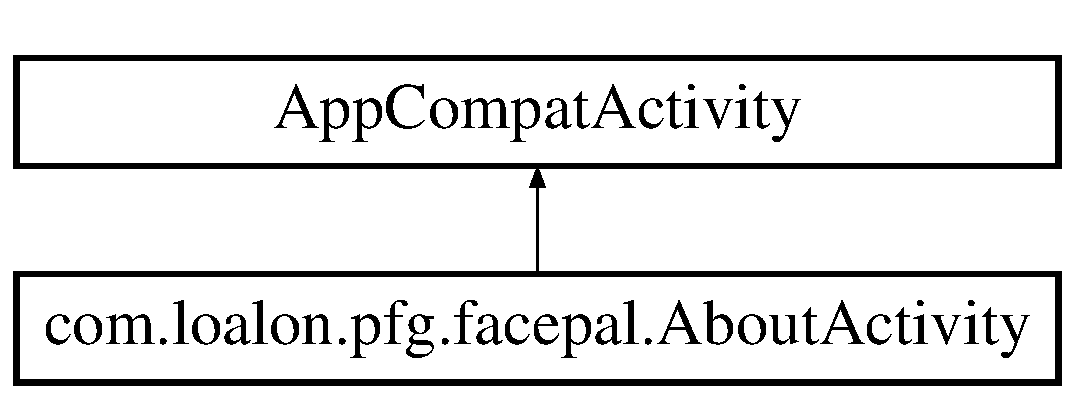
\includegraphics[height=2.000000cm]{classcom_1_1loalon_1_1pfg_1_1facepal_1_1_about_activity}
\end{center}
\end{figure}
\subsection*{Métodos protegidos}
\begin{DoxyCompactItemize}
\item 
void \mbox{\hyperlink{classcom_1_1loalon_1_1pfg_1_1facepal_1_1_about_activity_aaa1889e75b4be597a6e54ec668c03b03}{on\+Create}} (Bundle saved\+Instance\+State)
\end{DoxyCompactItemize}


\subsection{Descripción detallada}
Crea la actividad correspondiente para la pantalla acerca de... 

Created by Alonso on 03/04/2018. \begin{DoxyAuthor}{Autor}
Alonso Serrano 
\end{DoxyAuthor}
\begin{DoxyVersion}{Versión}
180403 
\end{DoxyVersion}


\subsection{Documentación de las funciones miembro}
\mbox{\Hypertarget{classcom_1_1loalon_1_1pfg_1_1facepal_1_1_about_activity_aaa1889e75b4be597a6e54ec668c03b03}\label{classcom_1_1loalon_1_1pfg_1_1facepal_1_1_about_activity_aaa1889e75b4be597a6e54ec668c03b03}} 
\index{com\+::loalon\+::pfg\+::facepal\+::\+About\+Activity@{com\+::loalon\+::pfg\+::facepal\+::\+About\+Activity}!on\+Create@{on\+Create}}
\index{on\+Create@{on\+Create}!com\+::loalon\+::pfg\+::facepal\+::\+About\+Activity@{com\+::loalon\+::pfg\+::facepal\+::\+About\+Activity}}
\subsubsection{\texorpdfstring{on\+Create()}{onCreate()}}
{\footnotesize\ttfamily void com.\+loalon.\+pfg.\+facepal.\+About\+Activity.\+on\+Create (\begin{DoxyParamCaption}\item[{Bundle}]{saved\+Instance\+State }\end{DoxyParamCaption})\hspace{0.3cm}{\ttfamily [protected]}}


\hypertarget{classcom_1_1loalon_1_1pfg_1_1facepal_1_1_app_compat_preference_activity}{}\section{Referencia de la Clase com.\+loalon.\+pfg.\+facepal.\+App\+Compat\+Preference\+Activity}
\label{classcom_1_1loalon_1_1pfg_1_1facepal_1_1_app_compat_preference_activity}\index{com.\+loalon.\+pfg.\+facepal.\+App\+Compat\+Preference\+Activity@{com.\+loalon.\+pfg.\+facepal.\+App\+Compat\+Preference\+Activity}}


Creada por Android Studio para implementar el menu de configuración.  


Diagrama de herencias de com.\+loalon.\+pfg.\+facepal.\+App\+Compat\+Preference\+Activity\begin{figure}[H]
\begin{center}
\leavevmode
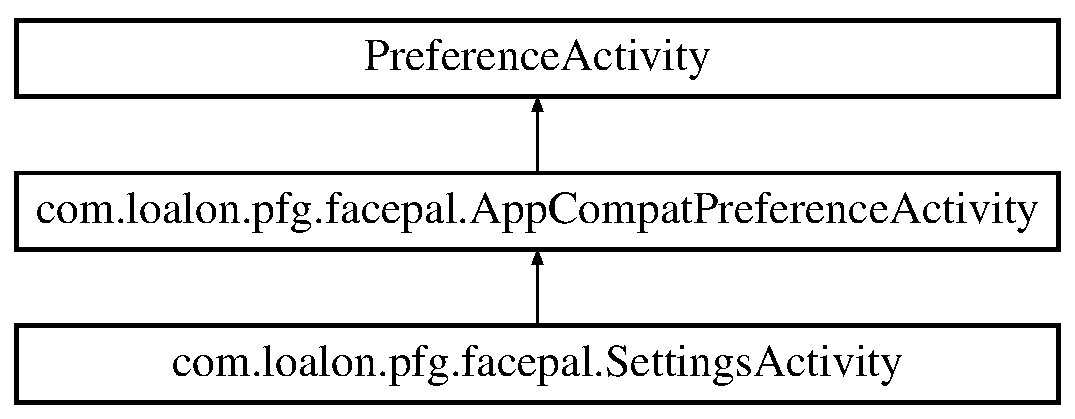
\includegraphics[height=3.000000cm]{classcom_1_1loalon_1_1pfg_1_1facepal_1_1_app_compat_preference_activity}
\end{center}
\end{figure}
\subsection*{Métodos públicos}
\begin{DoxyCompactItemize}
\item 
Action\+Bar \mbox{\hyperlink{classcom_1_1loalon_1_1pfg_1_1facepal_1_1_app_compat_preference_activity_afe58ba3051d87d3f3f6293995a31b429}{get\+Support\+Action\+Bar}} ()
\item 
void \mbox{\hyperlink{classcom_1_1loalon_1_1pfg_1_1facepal_1_1_app_compat_preference_activity_aac76dd0bd0fdcd1a027481856c085cd5}{set\+Support\+Action\+Bar}} (@Nullable Toolbar toolbar)
\item 
Menu\+Inflater \mbox{\hyperlink{classcom_1_1loalon_1_1pfg_1_1facepal_1_1_app_compat_preference_activity_af8c10bed11f19e960e5c30e67ba8996e}{get\+Menu\+Inflater}} ()
\item 
void \mbox{\hyperlink{classcom_1_1loalon_1_1pfg_1_1facepal_1_1_app_compat_preference_activity_aaaa2c55c420cd029906a1ec249a2db62}{set\+Content\+View}} (@Layout\+Res int layout\+Res\+ID)
\item 
void \mbox{\hyperlink{classcom_1_1loalon_1_1pfg_1_1facepal_1_1_app_compat_preference_activity_acb8ea15f72b5f052ef347cba2b8ead7a}{set\+Content\+View}} (View view)
\item 
void \mbox{\hyperlink{classcom_1_1loalon_1_1pfg_1_1facepal_1_1_app_compat_preference_activity_ae35d9258f0c07d79e4f8c9f16ac196e8}{set\+Content\+View}} (View view, View\+Group.\+Layout\+Params params)
\item 
void \mbox{\hyperlink{classcom_1_1loalon_1_1pfg_1_1facepal_1_1_app_compat_preference_activity_ac0e4a7ebdb9b70dfc44bf734abcf5039}{add\+Content\+View}} (View view, View\+Group.\+Layout\+Params params)
\item 
void \mbox{\hyperlink{classcom_1_1loalon_1_1pfg_1_1facepal_1_1_app_compat_preference_activity_a4dde4dbc997134f057d91b419beb859a}{on\+Configuration\+Changed}} (Configuration new\+Config)
\item 
void \mbox{\hyperlink{classcom_1_1loalon_1_1pfg_1_1facepal_1_1_app_compat_preference_activity_a330510859637ddbad639accf7ad1d412}{invalidate\+Options\+Menu}} ()
\end{DoxyCompactItemize}
\subsection*{Métodos protegidos}
\begin{DoxyCompactItemize}
\item 
void \mbox{\hyperlink{classcom_1_1loalon_1_1pfg_1_1facepal_1_1_app_compat_preference_activity_a4a7f2389e0796a1f1e758757b7ab99da}{on\+Create}} (Bundle saved\+Instance\+State)
\item 
void \mbox{\hyperlink{classcom_1_1loalon_1_1pfg_1_1facepal_1_1_app_compat_preference_activity_a89836ac30390948fe965d78d01530e77}{on\+Post\+Create}} (Bundle saved\+Instance\+State)
\item 
void \mbox{\hyperlink{classcom_1_1loalon_1_1pfg_1_1facepal_1_1_app_compat_preference_activity_a61539bdd250137ec5e3ff7a4dfee921a}{on\+Post\+Resume}} ()
\item 
void \mbox{\hyperlink{classcom_1_1loalon_1_1pfg_1_1facepal_1_1_app_compat_preference_activity_a3c4ede4b0fa997103ae6dc74ada97383}{on\+Title\+Changed}} (Char\+Sequence title, int color)
\item 
void \mbox{\hyperlink{classcom_1_1loalon_1_1pfg_1_1facepal_1_1_app_compat_preference_activity_a2da7c9998f2e5ba7ba7095a6060fbdb3}{on\+Stop}} ()
\item 
void \mbox{\hyperlink{classcom_1_1loalon_1_1pfg_1_1facepal_1_1_app_compat_preference_activity_ac91436db18f3546edc83d2933bc3a3af}{on\+Destroy}} ()
\end{DoxyCompactItemize}


\subsection{Descripción detallada}
Creada por Android Studio para implementar el menu de configuración. 

Created by Alonso on 28/03/2018. \begin{DoxyAuthor}{Autor}
Alonso Serrano 
\end{DoxyAuthor}
\begin{DoxyVersion}{Versión}
180328 A \mbox{\hyperlink{}{android.\+preference.\+Preference\+Activity}} which implements and proxies the necessary calls to be used with App\+Compat. 
\end{DoxyVersion}


\subsection{Documentación de las funciones miembro}
\mbox{\Hypertarget{classcom_1_1loalon_1_1pfg_1_1facepal_1_1_app_compat_preference_activity_ac0e4a7ebdb9b70dfc44bf734abcf5039}\label{classcom_1_1loalon_1_1pfg_1_1facepal_1_1_app_compat_preference_activity_ac0e4a7ebdb9b70dfc44bf734abcf5039}} 
\index{com\+::loalon\+::pfg\+::facepal\+::\+App\+Compat\+Preference\+Activity@{com\+::loalon\+::pfg\+::facepal\+::\+App\+Compat\+Preference\+Activity}!add\+Content\+View@{add\+Content\+View}}
\index{add\+Content\+View@{add\+Content\+View}!com\+::loalon\+::pfg\+::facepal\+::\+App\+Compat\+Preference\+Activity@{com\+::loalon\+::pfg\+::facepal\+::\+App\+Compat\+Preference\+Activity}}
\subsubsection{\texorpdfstring{add\+Content\+View()}{addContentView()}}
{\footnotesize\ttfamily void com.\+loalon.\+pfg.\+facepal.\+App\+Compat\+Preference\+Activity.\+add\+Content\+View (\begin{DoxyParamCaption}\item[{View}]{view,  }\item[{View\+Group.\+Layout\+Params}]{params }\end{DoxyParamCaption})}

\mbox{\Hypertarget{classcom_1_1loalon_1_1pfg_1_1facepal_1_1_app_compat_preference_activity_af8c10bed11f19e960e5c30e67ba8996e}\label{classcom_1_1loalon_1_1pfg_1_1facepal_1_1_app_compat_preference_activity_af8c10bed11f19e960e5c30e67ba8996e}} 
\index{com\+::loalon\+::pfg\+::facepal\+::\+App\+Compat\+Preference\+Activity@{com\+::loalon\+::pfg\+::facepal\+::\+App\+Compat\+Preference\+Activity}!get\+Menu\+Inflater@{get\+Menu\+Inflater}}
\index{get\+Menu\+Inflater@{get\+Menu\+Inflater}!com\+::loalon\+::pfg\+::facepal\+::\+App\+Compat\+Preference\+Activity@{com\+::loalon\+::pfg\+::facepal\+::\+App\+Compat\+Preference\+Activity}}
\subsubsection{\texorpdfstring{get\+Menu\+Inflater()}{getMenuInflater()}}
{\footnotesize\ttfamily Menu\+Inflater com.\+loalon.\+pfg.\+facepal.\+App\+Compat\+Preference\+Activity.\+get\+Menu\+Inflater (\begin{DoxyParamCaption}{ }\end{DoxyParamCaption})}

\mbox{\Hypertarget{classcom_1_1loalon_1_1pfg_1_1facepal_1_1_app_compat_preference_activity_afe58ba3051d87d3f3f6293995a31b429}\label{classcom_1_1loalon_1_1pfg_1_1facepal_1_1_app_compat_preference_activity_afe58ba3051d87d3f3f6293995a31b429}} 
\index{com\+::loalon\+::pfg\+::facepal\+::\+App\+Compat\+Preference\+Activity@{com\+::loalon\+::pfg\+::facepal\+::\+App\+Compat\+Preference\+Activity}!get\+Support\+Action\+Bar@{get\+Support\+Action\+Bar}}
\index{get\+Support\+Action\+Bar@{get\+Support\+Action\+Bar}!com\+::loalon\+::pfg\+::facepal\+::\+App\+Compat\+Preference\+Activity@{com\+::loalon\+::pfg\+::facepal\+::\+App\+Compat\+Preference\+Activity}}
\subsubsection{\texorpdfstring{get\+Support\+Action\+Bar()}{getSupportActionBar()}}
{\footnotesize\ttfamily Action\+Bar com.\+loalon.\+pfg.\+facepal.\+App\+Compat\+Preference\+Activity.\+get\+Support\+Action\+Bar (\begin{DoxyParamCaption}{ }\end{DoxyParamCaption})}

\mbox{\Hypertarget{classcom_1_1loalon_1_1pfg_1_1facepal_1_1_app_compat_preference_activity_a330510859637ddbad639accf7ad1d412}\label{classcom_1_1loalon_1_1pfg_1_1facepal_1_1_app_compat_preference_activity_a330510859637ddbad639accf7ad1d412}} 
\index{com\+::loalon\+::pfg\+::facepal\+::\+App\+Compat\+Preference\+Activity@{com\+::loalon\+::pfg\+::facepal\+::\+App\+Compat\+Preference\+Activity}!invalidate\+Options\+Menu@{invalidate\+Options\+Menu}}
\index{invalidate\+Options\+Menu@{invalidate\+Options\+Menu}!com\+::loalon\+::pfg\+::facepal\+::\+App\+Compat\+Preference\+Activity@{com\+::loalon\+::pfg\+::facepal\+::\+App\+Compat\+Preference\+Activity}}
\subsubsection{\texorpdfstring{invalidate\+Options\+Menu()}{invalidateOptionsMenu()}}
{\footnotesize\ttfamily void com.\+loalon.\+pfg.\+facepal.\+App\+Compat\+Preference\+Activity.\+invalidate\+Options\+Menu (\begin{DoxyParamCaption}{ }\end{DoxyParamCaption})}

\mbox{\Hypertarget{classcom_1_1loalon_1_1pfg_1_1facepal_1_1_app_compat_preference_activity_a4dde4dbc997134f057d91b419beb859a}\label{classcom_1_1loalon_1_1pfg_1_1facepal_1_1_app_compat_preference_activity_a4dde4dbc997134f057d91b419beb859a}} 
\index{com\+::loalon\+::pfg\+::facepal\+::\+App\+Compat\+Preference\+Activity@{com\+::loalon\+::pfg\+::facepal\+::\+App\+Compat\+Preference\+Activity}!on\+Configuration\+Changed@{on\+Configuration\+Changed}}
\index{on\+Configuration\+Changed@{on\+Configuration\+Changed}!com\+::loalon\+::pfg\+::facepal\+::\+App\+Compat\+Preference\+Activity@{com\+::loalon\+::pfg\+::facepal\+::\+App\+Compat\+Preference\+Activity}}
\subsubsection{\texorpdfstring{on\+Configuration\+Changed()}{onConfigurationChanged()}}
{\footnotesize\ttfamily void com.\+loalon.\+pfg.\+facepal.\+App\+Compat\+Preference\+Activity.\+on\+Configuration\+Changed (\begin{DoxyParamCaption}\item[{Configuration}]{new\+Config }\end{DoxyParamCaption})}

\mbox{\Hypertarget{classcom_1_1loalon_1_1pfg_1_1facepal_1_1_app_compat_preference_activity_a4a7f2389e0796a1f1e758757b7ab99da}\label{classcom_1_1loalon_1_1pfg_1_1facepal_1_1_app_compat_preference_activity_a4a7f2389e0796a1f1e758757b7ab99da}} 
\index{com\+::loalon\+::pfg\+::facepal\+::\+App\+Compat\+Preference\+Activity@{com\+::loalon\+::pfg\+::facepal\+::\+App\+Compat\+Preference\+Activity}!on\+Create@{on\+Create}}
\index{on\+Create@{on\+Create}!com\+::loalon\+::pfg\+::facepal\+::\+App\+Compat\+Preference\+Activity@{com\+::loalon\+::pfg\+::facepal\+::\+App\+Compat\+Preference\+Activity}}
\subsubsection{\texorpdfstring{on\+Create()}{onCreate()}}
{\footnotesize\ttfamily void com.\+loalon.\+pfg.\+facepal.\+App\+Compat\+Preference\+Activity.\+on\+Create (\begin{DoxyParamCaption}\item[{Bundle}]{saved\+Instance\+State }\end{DoxyParamCaption})\hspace{0.3cm}{\ttfamily [protected]}}

\mbox{\Hypertarget{classcom_1_1loalon_1_1pfg_1_1facepal_1_1_app_compat_preference_activity_ac91436db18f3546edc83d2933bc3a3af}\label{classcom_1_1loalon_1_1pfg_1_1facepal_1_1_app_compat_preference_activity_ac91436db18f3546edc83d2933bc3a3af}} 
\index{com\+::loalon\+::pfg\+::facepal\+::\+App\+Compat\+Preference\+Activity@{com\+::loalon\+::pfg\+::facepal\+::\+App\+Compat\+Preference\+Activity}!on\+Destroy@{on\+Destroy}}
\index{on\+Destroy@{on\+Destroy}!com\+::loalon\+::pfg\+::facepal\+::\+App\+Compat\+Preference\+Activity@{com\+::loalon\+::pfg\+::facepal\+::\+App\+Compat\+Preference\+Activity}}
\subsubsection{\texorpdfstring{on\+Destroy()}{onDestroy()}}
{\footnotesize\ttfamily void com.\+loalon.\+pfg.\+facepal.\+App\+Compat\+Preference\+Activity.\+on\+Destroy (\begin{DoxyParamCaption}{ }\end{DoxyParamCaption})\hspace{0.3cm}{\ttfamily [protected]}}

\mbox{\Hypertarget{classcom_1_1loalon_1_1pfg_1_1facepal_1_1_app_compat_preference_activity_a89836ac30390948fe965d78d01530e77}\label{classcom_1_1loalon_1_1pfg_1_1facepal_1_1_app_compat_preference_activity_a89836ac30390948fe965d78d01530e77}} 
\index{com\+::loalon\+::pfg\+::facepal\+::\+App\+Compat\+Preference\+Activity@{com\+::loalon\+::pfg\+::facepal\+::\+App\+Compat\+Preference\+Activity}!on\+Post\+Create@{on\+Post\+Create}}
\index{on\+Post\+Create@{on\+Post\+Create}!com\+::loalon\+::pfg\+::facepal\+::\+App\+Compat\+Preference\+Activity@{com\+::loalon\+::pfg\+::facepal\+::\+App\+Compat\+Preference\+Activity}}
\subsubsection{\texorpdfstring{on\+Post\+Create()}{onPostCreate()}}
{\footnotesize\ttfamily void com.\+loalon.\+pfg.\+facepal.\+App\+Compat\+Preference\+Activity.\+on\+Post\+Create (\begin{DoxyParamCaption}\item[{Bundle}]{saved\+Instance\+State }\end{DoxyParamCaption})\hspace{0.3cm}{\ttfamily [protected]}}

\mbox{\Hypertarget{classcom_1_1loalon_1_1pfg_1_1facepal_1_1_app_compat_preference_activity_a61539bdd250137ec5e3ff7a4dfee921a}\label{classcom_1_1loalon_1_1pfg_1_1facepal_1_1_app_compat_preference_activity_a61539bdd250137ec5e3ff7a4dfee921a}} 
\index{com\+::loalon\+::pfg\+::facepal\+::\+App\+Compat\+Preference\+Activity@{com\+::loalon\+::pfg\+::facepal\+::\+App\+Compat\+Preference\+Activity}!on\+Post\+Resume@{on\+Post\+Resume}}
\index{on\+Post\+Resume@{on\+Post\+Resume}!com\+::loalon\+::pfg\+::facepal\+::\+App\+Compat\+Preference\+Activity@{com\+::loalon\+::pfg\+::facepal\+::\+App\+Compat\+Preference\+Activity}}
\subsubsection{\texorpdfstring{on\+Post\+Resume()}{onPostResume()}}
{\footnotesize\ttfamily void com.\+loalon.\+pfg.\+facepal.\+App\+Compat\+Preference\+Activity.\+on\+Post\+Resume (\begin{DoxyParamCaption}{ }\end{DoxyParamCaption})\hspace{0.3cm}{\ttfamily [protected]}}

\mbox{\Hypertarget{classcom_1_1loalon_1_1pfg_1_1facepal_1_1_app_compat_preference_activity_a2da7c9998f2e5ba7ba7095a6060fbdb3}\label{classcom_1_1loalon_1_1pfg_1_1facepal_1_1_app_compat_preference_activity_a2da7c9998f2e5ba7ba7095a6060fbdb3}} 
\index{com\+::loalon\+::pfg\+::facepal\+::\+App\+Compat\+Preference\+Activity@{com\+::loalon\+::pfg\+::facepal\+::\+App\+Compat\+Preference\+Activity}!on\+Stop@{on\+Stop}}
\index{on\+Stop@{on\+Stop}!com\+::loalon\+::pfg\+::facepal\+::\+App\+Compat\+Preference\+Activity@{com\+::loalon\+::pfg\+::facepal\+::\+App\+Compat\+Preference\+Activity}}
\subsubsection{\texorpdfstring{on\+Stop()}{onStop()}}
{\footnotesize\ttfamily void com.\+loalon.\+pfg.\+facepal.\+App\+Compat\+Preference\+Activity.\+on\+Stop (\begin{DoxyParamCaption}{ }\end{DoxyParamCaption})\hspace{0.3cm}{\ttfamily [protected]}}

\mbox{\Hypertarget{classcom_1_1loalon_1_1pfg_1_1facepal_1_1_app_compat_preference_activity_a3c4ede4b0fa997103ae6dc74ada97383}\label{classcom_1_1loalon_1_1pfg_1_1facepal_1_1_app_compat_preference_activity_a3c4ede4b0fa997103ae6dc74ada97383}} 
\index{com\+::loalon\+::pfg\+::facepal\+::\+App\+Compat\+Preference\+Activity@{com\+::loalon\+::pfg\+::facepal\+::\+App\+Compat\+Preference\+Activity}!on\+Title\+Changed@{on\+Title\+Changed}}
\index{on\+Title\+Changed@{on\+Title\+Changed}!com\+::loalon\+::pfg\+::facepal\+::\+App\+Compat\+Preference\+Activity@{com\+::loalon\+::pfg\+::facepal\+::\+App\+Compat\+Preference\+Activity}}
\subsubsection{\texorpdfstring{on\+Title\+Changed()}{onTitleChanged()}}
{\footnotesize\ttfamily void com.\+loalon.\+pfg.\+facepal.\+App\+Compat\+Preference\+Activity.\+on\+Title\+Changed (\begin{DoxyParamCaption}\item[{Char\+Sequence}]{title,  }\item[{int}]{color }\end{DoxyParamCaption})\hspace{0.3cm}{\ttfamily [protected]}}

\mbox{\Hypertarget{classcom_1_1loalon_1_1pfg_1_1facepal_1_1_app_compat_preference_activity_aaaa2c55c420cd029906a1ec249a2db62}\label{classcom_1_1loalon_1_1pfg_1_1facepal_1_1_app_compat_preference_activity_aaaa2c55c420cd029906a1ec249a2db62}} 
\index{com\+::loalon\+::pfg\+::facepal\+::\+App\+Compat\+Preference\+Activity@{com\+::loalon\+::pfg\+::facepal\+::\+App\+Compat\+Preference\+Activity}!set\+Content\+View@{set\+Content\+View}}
\index{set\+Content\+View@{set\+Content\+View}!com\+::loalon\+::pfg\+::facepal\+::\+App\+Compat\+Preference\+Activity@{com\+::loalon\+::pfg\+::facepal\+::\+App\+Compat\+Preference\+Activity}}
\subsubsection{\texorpdfstring{set\+Content\+View()}{setContentView()}\hspace{0.1cm}{\footnotesize\ttfamily [1/3]}}
{\footnotesize\ttfamily void com.\+loalon.\+pfg.\+facepal.\+App\+Compat\+Preference\+Activity.\+set\+Content\+View (\begin{DoxyParamCaption}\item[{@Layout\+Res int}]{layout\+Res\+ID }\end{DoxyParamCaption})}

\mbox{\Hypertarget{classcom_1_1loalon_1_1pfg_1_1facepal_1_1_app_compat_preference_activity_acb8ea15f72b5f052ef347cba2b8ead7a}\label{classcom_1_1loalon_1_1pfg_1_1facepal_1_1_app_compat_preference_activity_acb8ea15f72b5f052ef347cba2b8ead7a}} 
\index{com\+::loalon\+::pfg\+::facepal\+::\+App\+Compat\+Preference\+Activity@{com\+::loalon\+::pfg\+::facepal\+::\+App\+Compat\+Preference\+Activity}!set\+Content\+View@{set\+Content\+View}}
\index{set\+Content\+View@{set\+Content\+View}!com\+::loalon\+::pfg\+::facepal\+::\+App\+Compat\+Preference\+Activity@{com\+::loalon\+::pfg\+::facepal\+::\+App\+Compat\+Preference\+Activity}}
\subsubsection{\texorpdfstring{set\+Content\+View()}{setContentView()}\hspace{0.1cm}{\footnotesize\ttfamily [2/3]}}
{\footnotesize\ttfamily void com.\+loalon.\+pfg.\+facepal.\+App\+Compat\+Preference\+Activity.\+set\+Content\+View (\begin{DoxyParamCaption}\item[{View}]{view }\end{DoxyParamCaption})}

\mbox{\Hypertarget{classcom_1_1loalon_1_1pfg_1_1facepal_1_1_app_compat_preference_activity_ae35d9258f0c07d79e4f8c9f16ac196e8}\label{classcom_1_1loalon_1_1pfg_1_1facepal_1_1_app_compat_preference_activity_ae35d9258f0c07d79e4f8c9f16ac196e8}} 
\index{com\+::loalon\+::pfg\+::facepal\+::\+App\+Compat\+Preference\+Activity@{com\+::loalon\+::pfg\+::facepal\+::\+App\+Compat\+Preference\+Activity}!set\+Content\+View@{set\+Content\+View}}
\index{set\+Content\+View@{set\+Content\+View}!com\+::loalon\+::pfg\+::facepal\+::\+App\+Compat\+Preference\+Activity@{com\+::loalon\+::pfg\+::facepal\+::\+App\+Compat\+Preference\+Activity}}
\subsubsection{\texorpdfstring{set\+Content\+View()}{setContentView()}\hspace{0.1cm}{\footnotesize\ttfamily [3/3]}}
{\footnotesize\ttfamily void com.\+loalon.\+pfg.\+facepal.\+App\+Compat\+Preference\+Activity.\+set\+Content\+View (\begin{DoxyParamCaption}\item[{View}]{view,  }\item[{View\+Group.\+Layout\+Params}]{params }\end{DoxyParamCaption})}

\mbox{\Hypertarget{classcom_1_1loalon_1_1pfg_1_1facepal_1_1_app_compat_preference_activity_aac76dd0bd0fdcd1a027481856c085cd5}\label{classcom_1_1loalon_1_1pfg_1_1facepal_1_1_app_compat_preference_activity_aac76dd0bd0fdcd1a027481856c085cd5}} 
\index{com\+::loalon\+::pfg\+::facepal\+::\+App\+Compat\+Preference\+Activity@{com\+::loalon\+::pfg\+::facepal\+::\+App\+Compat\+Preference\+Activity}!set\+Support\+Action\+Bar@{set\+Support\+Action\+Bar}}
\index{set\+Support\+Action\+Bar@{set\+Support\+Action\+Bar}!com\+::loalon\+::pfg\+::facepal\+::\+App\+Compat\+Preference\+Activity@{com\+::loalon\+::pfg\+::facepal\+::\+App\+Compat\+Preference\+Activity}}
\subsubsection{\texorpdfstring{set\+Support\+Action\+Bar()}{setSupportActionBar()}}
{\footnotesize\ttfamily void com.\+loalon.\+pfg.\+facepal.\+App\+Compat\+Preference\+Activity.\+set\+Support\+Action\+Bar (\begin{DoxyParamCaption}\item[{@Nullable Toolbar}]{toolbar }\end{DoxyParamCaption})}


\hypertarget{classcom_1_1loalon_1_1pfg_1_1facepal_1_1_async_add_face}{}\section{Referencia de la Clase com.\+loalon.\+pfg.\+facepal.\+Async\+Add\+Face}
\label{classcom_1_1loalon_1_1pfg_1_1facepal_1_1_async_add_face}\index{com.\+loalon.\+pfg.\+facepal.\+Async\+Add\+Face@{com.\+loalon.\+pfg.\+facepal.\+Async\+Add\+Face}}


Tarea asincrona de añadir cara.  


Diagrama de herencias de com.\+loalon.\+pfg.\+facepal.\+Async\+Add\+Face\begin{figure}[H]
\begin{center}
\leavevmode
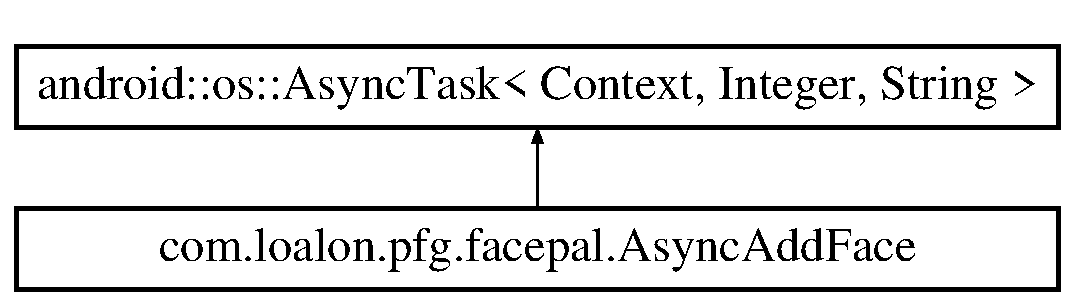
\includegraphics[height=2.000000cm]{classcom_1_1loalon_1_1pfg_1_1facepal_1_1_async_add_face}
\end{center}
\end{figure}
\subsection*{Métodos públicos}
\begin{DoxyCompactItemize}
\item 
\mbox{\hyperlink{classcom_1_1loalon_1_1pfg_1_1facepal_1_1_async_add_face_a06192a655442f59a2e6e59f8467e7023}{Async\+Add\+Face}} (Context context, View view, String group\+Name, String face\+Name, Bitmap bitmap)
\end{DoxyCompactItemize}
\subsection*{Métodos protegidos}
\begin{DoxyCompactItemize}
\item 
void \mbox{\hyperlink{classcom_1_1loalon_1_1pfg_1_1facepal_1_1_async_add_face_a7429c6c8e7ccbad90ee8d9e773759eca}{on\+Pre\+Execute}} ()
\item 
String \mbox{\hyperlink{classcom_1_1loalon_1_1pfg_1_1facepal_1_1_async_add_face_aeb5252530e4cbcacbe3b9a6be3e2f0f2}{do\+In\+Background}} (Context... params)
\item 
void \mbox{\hyperlink{classcom_1_1loalon_1_1pfg_1_1facepal_1_1_async_add_face_abde1ae4ecac2cbf630715dbf1fd88d36}{on\+Post\+Execute}} (String result)
\end{DoxyCompactItemize}


\subsection{Descripción detallada}
Tarea asincrona de añadir cara. 

Created by Alonso on 09/04/2018. \begin{DoxyAuthor}{Autor}
Alonso Serrano 
\end{DoxyAuthor}
\begin{DoxyVersion}{Versión}
180415 
\end{DoxyVersion}


\subsection{Documentación del constructor y destructor}
\mbox{\Hypertarget{classcom_1_1loalon_1_1pfg_1_1facepal_1_1_async_add_face_a06192a655442f59a2e6e59f8467e7023}\label{classcom_1_1loalon_1_1pfg_1_1facepal_1_1_async_add_face_a06192a655442f59a2e6e59f8467e7023}} 
\index{com\+::loalon\+::pfg\+::facepal\+::\+Async\+Add\+Face@{com\+::loalon\+::pfg\+::facepal\+::\+Async\+Add\+Face}!Async\+Add\+Face@{Async\+Add\+Face}}
\index{Async\+Add\+Face@{Async\+Add\+Face}!com\+::loalon\+::pfg\+::facepal\+::\+Async\+Add\+Face@{com\+::loalon\+::pfg\+::facepal\+::\+Async\+Add\+Face}}
\subsubsection{\texorpdfstring{Async\+Add\+Face()}{AsyncAddFace()}}
{\footnotesize\ttfamily com.\+loalon.\+pfg.\+facepal.\+Async\+Add\+Face.\+Async\+Add\+Face (\begin{DoxyParamCaption}\item[{Context}]{context,  }\item[{View}]{view,  }\item[{String}]{group\+Name,  }\item[{String}]{face\+Name,  }\item[{Bitmap}]{bitmap }\end{DoxyParamCaption})}


\begin{DoxyParams}{Parámetros}
{\em context} & Contexto de la aplicacion \\
\hline
{\em view} & view don de apareceran los mensajes \\
\hline
{\em group\+Name} & nombre del grupo \\
\hline
{\em face\+Name} & nombre de la persona a la que se agregara la cara \\
\hline
{\em bitmap} & imagen de la cara a añadir \\
\hline
\end{DoxyParams}


\subsection{Documentación de las funciones miembro}
\mbox{\Hypertarget{classcom_1_1loalon_1_1pfg_1_1facepal_1_1_async_add_face_aeb5252530e4cbcacbe3b9a6be3e2f0f2}\label{classcom_1_1loalon_1_1pfg_1_1facepal_1_1_async_add_face_aeb5252530e4cbcacbe3b9a6be3e2f0f2}} 
\index{com\+::loalon\+::pfg\+::facepal\+::\+Async\+Add\+Face@{com\+::loalon\+::pfg\+::facepal\+::\+Async\+Add\+Face}!do\+In\+Background@{do\+In\+Background}}
\index{do\+In\+Background@{do\+In\+Background}!com\+::loalon\+::pfg\+::facepal\+::\+Async\+Add\+Face@{com\+::loalon\+::pfg\+::facepal\+::\+Async\+Add\+Face}}
\subsubsection{\texorpdfstring{do\+In\+Background()}{doInBackground()}}
{\footnotesize\ttfamily String com.\+loalon.\+pfg.\+facepal.\+Async\+Add\+Face.\+do\+In\+Background (\begin{DoxyParamCaption}\item[{Context...}]{params }\end{DoxyParamCaption})\hspace{0.3cm}{\ttfamily [protected]}}

\mbox{\Hypertarget{classcom_1_1loalon_1_1pfg_1_1facepal_1_1_async_add_face_abde1ae4ecac2cbf630715dbf1fd88d36}\label{classcom_1_1loalon_1_1pfg_1_1facepal_1_1_async_add_face_abde1ae4ecac2cbf630715dbf1fd88d36}} 
\index{com\+::loalon\+::pfg\+::facepal\+::\+Async\+Add\+Face@{com\+::loalon\+::pfg\+::facepal\+::\+Async\+Add\+Face}!on\+Post\+Execute@{on\+Post\+Execute}}
\index{on\+Post\+Execute@{on\+Post\+Execute}!com\+::loalon\+::pfg\+::facepal\+::\+Async\+Add\+Face@{com\+::loalon\+::pfg\+::facepal\+::\+Async\+Add\+Face}}
\subsubsection{\texorpdfstring{on\+Post\+Execute()}{onPostExecute()}}
{\footnotesize\ttfamily void com.\+loalon.\+pfg.\+facepal.\+Async\+Add\+Face.\+on\+Post\+Execute (\begin{DoxyParamCaption}\item[{String}]{result }\end{DoxyParamCaption})\hspace{0.3cm}{\ttfamily [protected]}}

\mbox{\Hypertarget{classcom_1_1loalon_1_1pfg_1_1facepal_1_1_async_add_face_a7429c6c8e7ccbad90ee8d9e773759eca}\label{classcom_1_1loalon_1_1pfg_1_1facepal_1_1_async_add_face_a7429c6c8e7ccbad90ee8d9e773759eca}} 
\index{com\+::loalon\+::pfg\+::facepal\+::\+Async\+Add\+Face@{com\+::loalon\+::pfg\+::facepal\+::\+Async\+Add\+Face}!on\+Pre\+Execute@{on\+Pre\+Execute}}
\index{on\+Pre\+Execute@{on\+Pre\+Execute}!com\+::loalon\+::pfg\+::facepal\+::\+Async\+Add\+Face@{com\+::loalon\+::pfg\+::facepal\+::\+Async\+Add\+Face}}
\subsubsection{\texorpdfstring{on\+Pre\+Execute()}{onPreExecute()}}
{\footnotesize\ttfamily void com.\+loalon.\+pfg.\+facepal.\+Async\+Add\+Face.\+on\+Pre\+Execute (\begin{DoxyParamCaption}{ }\end{DoxyParamCaption})\hspace{0.3cm}{\ttfamily [protected]}}


\hypertarget{classcom_1_1loalon_1_1pfg_1_1facepal_1_1_async_add_person}{}\section{Referencia de la Clase com.\+loalon.\+pfg.\+facepal.\+Async\+Add\+Person}
\label{classcom_1_1loalon_1_1pfg_1_1facepal_1_1_async_add_person}\index{com.\+loalon.\+pfg.\+facepal.\+Async\+Add\+Person@{com.\+loalon.\+pfg.\+facepal.\+Async\+Add\+Person}}


Tarea asincrona de añadir persona.  


Diagrama de herencias de com.\+loalon.\+pfg.\+facepal.\+Async\+Add\+Person\begin{figure}[H]
\begin{center}
\leavevmode
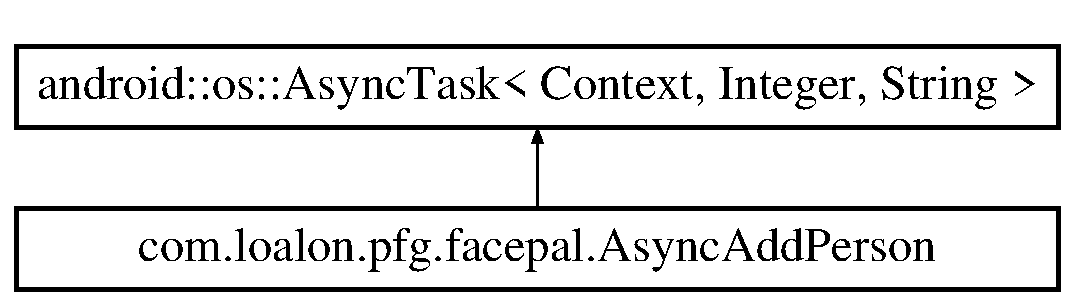
\includegraphics[height=2.000000cm]{classcom_1_1loalon_1_1pfg_1_1facepal_1_1_async_add_person}
\end{center}
\end{figure}
\subsection*{Métodos públicos}
\begin{DoxyCompactItemize}
\item 
\mbox{\hyperlink{classcom_1_1loalon_1_1pfg_1_1facepal_1_1_async_add_person_aa88098f2f6ee436d7b26b7d9d5432a58}{Async\+Add\+Person}} (Context context, View view, String group\+Name, String face\+Name, Bitmap bitmap)
\end{DoxyCompactItemize}
\subsection*{Métodos protegidos}
\begin{DoxyCompactItemize}
\item 
void \mbox{\hyperlink{classcom_1_1loalon_1_1pfg_1_1facepal_1_1_async_add_person_a6af153108c502542ce6465006795a1b2}{on\+Pre\+Execute}} ()
\item 
String \mbox{\hyperlink{classcom_1_1loalon_1_1pfg_1_1facepal_1_1_async_add_person_a15123e65e39ef6a2453bad1efd536614}{do\+In\+Background}} (Context... params)
\item 
void \mbox{\hyperlink{classcom_1_1loalon_1_1pfg_1_1facepal_1_1_async_add_person_a885607cbe0ea901fdc1d567da6067b89}{on\+Post\+Execute}} (String result)
\end{DoxyCompactItemize}


\subsection{Descripción detallada}
Tarea asincrona de añadir persona. 

Created by Alonso on 09/04/2018. \begin{DoxyAuthor}{Autor}
Alonso Serrano 
\end{DoxyAuthor}
\begin{DoxyVersion}{Versión}
180415 
\end{DoxyVersion}


\subsection{Documentación del constructor y destructor}
\mbox{\Hypertarget{classcom_1_1loalon_1_1pfg_1_1facepal_1_1_async_add_person_aa88098f2f6ee436d7b26b7d9d5432a58}\label{classcom_1_1loalon_1_1pfg_1_1facepal_1_1_async_add_person_aa88098f2f6ee436d7b26b7d9d5432a58}} 
\index{com\+::loalon\+::pfg\+::facepal\+::\+Async\+Add\+Person@{com\+::loalon\+::pfg\+::facepal\+::\+Async\+Add\+Person}!Async\+Add\+Person@{Async\+Add\+Person}}
\index{Async\+Add\+Person@{Async\+Add\+Person}!com\+::loalon\+::pfg\+::facepal\+::\+Async\+Add\+Person@{com\+::loalon\+::pfg\+::facepal\+::\+Async\+Add\+Person}}
\subsubsection{\texorpdfstring{Async\+Add\+Person()}{AsyncAddPerson()}}
{\footnotesize\ttfamily com.\+loalon.\+pfg.\+facepal.\+Async\+Add\+Person.\+Async\+Add\+Person (\begin{DoxyParamCaption}\item[{Context}]{context,  }\item[{View}]{view,  }\item[{String}]{group\+Name,  }\item[{String}]{face\+Name,  }\item[{Bitmap}]{bitmap }\end{DoxyParamCaption})}


\begin{DoxyParams}{Parámetros}
{\em context} & Contexto de la aplicacion \\
\hline
{\em view} & view don de apareceran los mensajes \\
\hline
{\em group\+Name} & nombre del grupo \\
\hline
{\em face\+Name} & nombre de la persona nueva \\
\hline
{\em bitmap} & imagen de la primera cara a añadir \\
\hline
\end{DoxyParams}


\subsection{Documentación de las funciones miembro}
\mbox{\Hypertarget{classcom_1_1loalon_1_1pfg_1_1facepal_1_1_async_add_person_a15123e65e39ef6a2453bad1efd536614}\label{classcom_1_1loalon_1_1pfg_1_1facepal_1_1_async_add_person_a15123e65e39ef6a2453bad1efd536614}} 
\index{com\+::loalon\+::pfg\+::facepal\+::\+Async\+Add\+Person@{com\+::loalon\+::pfg\+::facepal\+::\+Async\+Add\+Person}!do\+In\+Background@{do\+In\+Background}}
\index{do\+In\+Background@{do\+In\+Background}!com\+::loalon\+::pfg\+::facepal\+::\+Async\+Add\+Person@{com\+::loalon\+::pfg\+::facepal\+::\+Async\+Add\+Person}}
\subsubsection{\texorpdfstring{do\+In\+Background()}{doInBackground()}}
{\footnotesize\ttfamily String com.\+loalon.\+pfg.\+facepal.\+Async\+Add\+Person.\+do\+In\+Background (\begin{DoxyParamCaption}\item[{Context...}]{params }\end{DoxyParamCaption})\hspace{0.3cm}{\ttfamily [protected]}}

\mbox{\Hypertarget{classcom_1_1loalon_1_1pfg_1_1facepal_1_1_async_add_person_a885607cbe0ea901fdc1d567da6067b89}\label{classcom_1_1loalon_1_1pfg_1_1facepal_1_1_async_add_person_a885607cbe0ea901fdc1d567da6067b89}} 
\index{com\+::loalon\+::pfg\+::facepal\+::\+Async\+Add\+Person@{com\+::loalon\+::pfg\+::facepal\+::\+Async\+Add\+Person}!on\+Post\+Execute@{on\+Post\+Execute}}
\index{on\+Post\+Execute@{on\+Post\+Execute}!com\+::loalon\+::pfg\+::facepal\+::\+Async\+Add\+Person@{com\+::loalon\+::pfg\+::facepal\+::\+Async\+Add\+Person}}
\subsubsection{\texorpdfstring{on\+Post\+Execute()}{onPostExecute()}}
{\footnotesize\ttfamily void com.\+loalon.\+pfg.\+facepal.\+Async\+Add\+Person.\+on\+Post\+Execute (\begin{DoxyParamCaption}\item[{String}]{result }\end{DoxyParamCaption})\hspace{0.3cm}{\ttfamily [protected]}}

\mbox{\Hypertarget{classcom_1_1loalon_1_1pfg_1_1facepal_1_1_async_add_person_a6af153108c502542ce6465006795a1b2}\label{classcom_1_1loalon_1_1pfg_1_1facepal_1_1_async_add_person_a6af153108c502542ce6465006795a1b2}} 
\index{com\+::loalon\+::pfg\+::facepal\+::\+Async\+Add\+Person@{com\+::loalon\+::pfg\+::facepal\+::\+Async\+Add\+Person}!on\+Pre\+Execute@{on\+Pre\+Execute}}
\index{on\+Pre\+Execute@{on\+Pre\+Execute}!com\+::loalon\+::pfg\+::facepal\+::\+Async\+Add\+Person@{com\+::loalon\+::pfg\+::facepal\+::\+Async\+Add\+Person}}
\subsubsection{\texorpdfstring{on\+Pre\+Execute()}{onPreExecute()}}
{\footnotesize\ttfamily void com.\+loalon.\+pfg.\+facepal.\+Async\+Add\+Person.\+on\+Pre\+Execute (\begin{DoxyParamCaption}{ }\end{DoxyParamCaption})\hspace{0.3cm}{\ttfamily [protected]}}


\hypertarget{classcom_1_1loalon_1_1pfg_1_1facepal_1_1_async_face_croper}{}\section{Referencia de la Clase com.\+loalon.\+pfg.\+facepal.\+Async\+Face\+Croper}
\label{classcom_1_1loalon_1_1pfg_1_1facepal_1_1_async_face_croper}\index{com.\+loalon.\+pfg.\+facepal.\+Async\+Face\+Croper@{com.\+loalon.\+pfg.\+facepal.\+Async\+Face\+Croper}}


Tarea asincrona de recortar cara.  


Diagrama de herencias de com.\+loalon.\+pfg.\+facepal.\+Async\+Face\+Croper\begin{figure}[H]
\begin{center}
\leavevmode
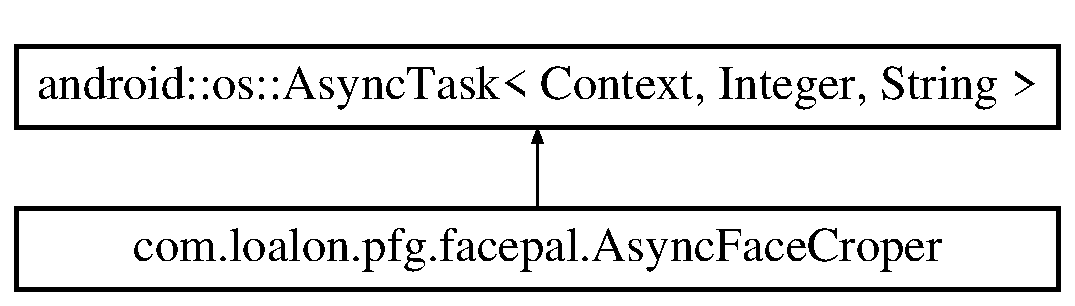
\includegraphics[height=2.000000cm]{classcom_1_1loalon_1_1pfg_1_1facepal_1_1_async_face_croper}
\end{center}
\end{figure}
\subsection*{Clases}
\begin{DoxyCompactItemize}
\item 
interface \mbox{\hyperlink{interfacecom_1_1loalon_1_1pfg_1_1facepal_1_1_async_face_croper_1_1_async_response}{Async\+Response}}
\end{DoxyCompactItemize}
\subsection*{Métodos públicos}
\begin{DoxyCompactItemize}
\item 
\mbox{\hyperlink{classcom_1_1loalon_1_1pfg_1_1facepal_1_1_async_face_croper_a3edb3637aee55bd3d224ff23dc9652d8}{Async\+Face\+Croper}} (Context context, Bitmap bitmap, Image\+View image\+View, \mbox{\hyperlink{interfacecom_1_1loalon_1_1pfg_1_1facepal_1_1_async_face_croper_1_1_async_response}{Async\+Response}} \mbox{\hyperlink{classcom_1_1loalon_1_1pfg_1_1facepal_1_1_async_face_croper_a11ee69c0d77c5662fb576d1a1547ca83}{delegate}})
\end{DoxyCompactItemize}
\subsection*{Atributos públicos}
\begin{DoxyCompactItemize}
\item 
\mbox{\hyperlink{interfacecom_1_1loalon_1_1pfg_1_1facepal_1_1_async_face_croper_1_1_async_response}{Async\+Response}} \mbox{\hyperlink{classcom_1_1loalon_1_1pfg_1_1facepal_1_1_async_face_croper_a11ee69c0d77c5662fb576d1a1547ca83}{delegate}} = null
\end{DoxyCompactItemize}
\subsection*{Métodos protegidos}
\begin{DoxyCompactItemize}
\item 
void \mbox{\hyperlink{classcom_1_1loalon_1_1pfg_1_1facepal_1_1_async_face_croper_a124ec9711412ee0c2748b7ad0ae3d7a2}{on\+Pre\+Execute}} ()
\item 
String \mbox{\hyperlink{classcom_1_1loalon_1_1pfg_1_1facepal_1_1_async_face_croper_ace858d5f1d68f8b06eb58770d26cdcbe}{do\+In\+Background}} (Context... params)
\item 
void \mbox{\hyperlink{classcom_1_1loalon_1_1pfg_1_1facepal_1_1_async_face_croper_ac0b81c27b11613192ae684ea6ffdbf43}{on\+Post\+Execute}} (String result)
\end{DoxyCompactItemize}


\subsection{Descripción detallada}
Tarea asincrona de recortar cara. 

Created by Alonso on 09/04/2018. \begin{DoxyAuthor}{Autor}
Alonso Serrano 
\end{DoxyAuthor}
\begin{DoxyVersion}{Versión}
180415 
\end{DoxyVersion}


\subsection{Documentación del constructor y destructor}
\mbox{\Hypertarget{classcom_1_1loalon_1_1pfg_1_1facepal_1_1_async_face_croper_a3edb3637aee55bd3d224ff23dc9652d8}\label{classcom_1_1loalon_1_1pfg_1_1facepal_1_1_async_face_croper_a3edb3637aee55bd3d224ff23dc9652d8}} 
\index{com\+::loalon\+::pfg\+::facepal\+::\+Async\+Face\+Croper@{com\+::loalon\+::pfg\+::facepal\+::\+Async\+Face\+Croper}!Async\+Face\+Croper@{Async\+Face\+Croper}}
\index{Async\+Face\+Croper@{Async\+Face\+Croper}!com\+::loalon\+::pfg\+::facepal\+::\+Async\+Face\+Croper@{com\+::loalon\+::pfg\+::facepal\+::\+Async\+Face\+Croper}}
\subsubsection{\texorpdfstring{Async\+Face\+Croper()}{AsyncFaceCroper()}}
{\footnotesize\ttfamily com.\+loalon.\+pfg.\+facepal.\+Async\+Face\+Croper.\+Async\+Face\+Croper (\begin{DoxyParamCaption}\item[{Context}]{context,  }\item[{Bitmap}]{bitmap,  }\item[{Image\+View}]{image\+View,  }\item[{\mbox{\hyperlink{interfacecom_1_1loalon_1_1pfg_1_1facepal_1_1_async_face_croper_1_1_async_response}{Async\+Response}}}]{delegate }\end{DoxyParamCaption})}



\subsection{Documentación de las funciones miembro}
\mbox{\Hypertarget{classcom_1_1loalon_1_1pfg_1_1facepal_1_1_async_face_croper_ace858d5f1d68f8b06eb58770d26cdcbe}\label{classcom_1_1loalon_1_1pfg_1_1facepal_1_1_async_face_croper_ace858d5f1d68f8b06eb58770d26cdcbe}} 
\index{com\+::loalon\+::pfg\+::facepal\+::\+Async\+Face\+Croper@{com\+::loalon\+::pfg\+::facepal\+::\+Async\+Face\+Croper}!do\+In\+Background@{do\+In\+Background}}
\index{do\+In\+Background@{do\+In\+Background}!com\+::loalon\+::pfg\+::facepal\+::\+Async\+Face\+Croper@{com\+::loalon\+::pfg\+::facepal\+::\+Async\+Face\+Croper}}
\subsubsection{\texorpdfstring{do\+In\+Background()}{doInBackground()}}
{\footnotesize\ttfamily String com.\+loalon.\+pfg.\+facepal.\+Async\+Face\+Croper.\+do\+In\+Background (\begin{DoxyParamCaption}\item[{Context...}]{params }\end{DoxyParamCaption})\hspace{0.3cm}{\ttfamily [protected]}}

\mbox{\Hypertarget{classcom_1_1loalon_1_1pfg_1_1facepal_1_1_async_face_croper_ac0b81c27b11613192ae684ea6ffdbf43}\label{classcom_1_1loalon_1_1pfg_1_1facepal_1_1_async_face_croper_ac0b81c27b11613192ae684ea6ffdbf43}} 
\index{com\+::loalon\+::pfg\+::facepal\+::\+Async\+Face\+Croper@{com\+::loalon\+::pfg\+::facepal\+::\+Async\+Face\+Croper}!on\+Post\+Execute@{on\+Post\+Execute}}
\index{on\+Post\+Execute@{on\+Post\+Execute}!com\+::loalon\+::pfg\+::facepal\+::\+Async\+Face\+Croper@{com\+::loalon\+::pfg\+::facepal\+::\+Async\+Face\+Croper}}
\subsubsection{\texorpdfstring{on\+Post\+Execute()}{onPostExecute()}}
{\footnotesize\ttfamily void com.\+loalon.\+pfg.\+facepal.\+Async\+Face\+Croper.\+on\+Post\+Execute (\begin{DoxyParamCaption}\item[{String}]{result }\end{DoxyParamCaption})\hspace{0.3cm}{\ttfamily [protected]}}

\mbox{\Hypertarget{classcom_1_1loalon_1_1pfg_1_1facepal_1_1_async_face_croper_a124ec9711412ee0c2748b7ad0ae3d7a2}\label{classcom_1_1loalon_1_1pfg_1_1facepal_1_1_async_face_croper_a124ec9711412ee0c2748b7ad0ae3d7a2}} 
\index{com\+::loalon\+::pfg\+::facepal\+::\+Async\+Face\+Croper@{com\+::loalon\+::pfg\+::facepal\+::\+Async\+Face\+Croper}!on\+Pre\+Execute@{on\+Pre\+Execute}}
\index{on\+Pre\+Execute@{on\+Pre\+Execute}!com\+::loalon\+::pfg\+::facepal\+::\+Async\+Face\+Croper@{com\+::loalon\+::pfg\+::facepal\+::\+Async\+Face\+Croper}}
\subsubsection{\texorpdfstring{on\+Pre\+Execute()}{onPreExecute()}}
{\footnotesize\ttfamily void com.\+loalon.\+pfg.\+facepal.\+Async\+Face\+Croper.\+on\+Pre\+Execute (\begin{DoxyParamCaption}{ }\end{DoxyParamCaption})\hspace{0.3cm}{\ttfamily [protected]}}



\subsection{Documentación de los datos miembro}
\mbox{\Hypertarget{classcom_1_1loalon_1_1pfg_1_1facepal_1_1_async_face_croper_a11ee69c0d77c5662fb576d1a1547ca83}\label{classcom_1_1loalon_1_1pfg_1_1facepal_1_1_async_face_croper_a11ee69c0d77c5662fb576d1a1547ca83}} 
\index{com\+::loalon\+::pfg\+::facepal\+::\+Async\+Face\+Croper@{com\+::loalon\+::pfg\+::facepal\+::\+Async\+Face\+Croper}!delegate@{delegate}}
\index{delegate@{delegate}!com\+::loalon\+::pfg\+::facepal\+::\+Async\+Face\+Croper@{com\+::loalon\+::pfg\+::facepal\+::\+Async\+Face\+Croper}}
\subsubsection{\texorpdfstring{delegate}{delegate}}
{\footnotesize\ttfamily \mbox{\hyperlink{interfacecom_1_1loalon_1_1pfg_1_1facepal_1_1_async_face_croper_1_1_async_response}{Async\+Response}} com.\+loalon.\+pfg.\+facepal.\+Async\+Face\+Croper.\+delegate = null}


\hypertarget{classcom_1_1loalon_1_1pfg_1_1facepal_1_1_async_face_detector}{}\section{Referencia de la Clase com.\+loalon.\+pfg.\+facepal.\+Async\+Face\+Detector}
\label{classcom_1_1loalon_1_1pfg_1_1facepal_1_1_async_face_detector}\index{com.\+loalon.\+pfg.\+facepal.\+Async\+Face\+Detector@{com.\+loalon.\+pfg.\+facepal.\+Async\+Face\+Detector}}


Tarea asincrona de D\+E\+T\+E\+C\+T\+AR cara.  


Diagrama de herencias de com.\+loalon.\+pfg.\+facepal.\+Async\+Face\+Detector\begin{figure}[H]
\begin{center}
\leavevmode
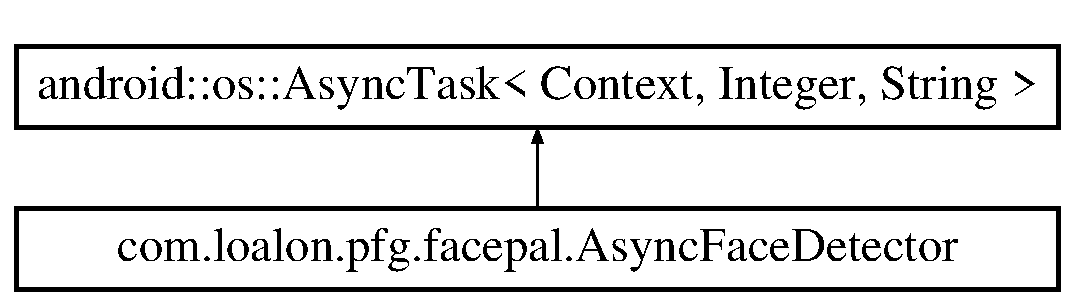
\includegraphics[height=2.000000cm]{classcom_1_1loalon_1_1pfg_1_1facepal_1_1_async_face_detector}
\end{center}
\end{figure}
\subsection*{Métodos públicos}
\begin{DoxyCompactItemize}
\item 
\mbox{\hyperlink{classcom_1_1loalon_1_1pfg_1_1facepal_1_1_async_face_detector_a80b8c1b69a8f4a0b3855d9e289626079}{Async\+Face\+Detector}} (Context context, View view, Bitmap bitmap)
\end{DoxyCompactItemize}
\subsection*{Métodos protegidos}
\begin{DoxyCompactItemize}
\item 
void \mbox{\hyperlink{classcom_1_1loalon_1_1pfg_1_1facepal_1_1_async_face_detector_a69b608adca8119418bfce881d9f4c8de}{on\+Pre\+Execute}} ()
\item 
String \mbox{\hyperlink{classcom_1_1loalon_1_1pfg_1_1facepal_1_1_async_face_detector_ad9f3deb7c59c258ea2b13d7f79699232}{do\+In\+Background}} (Context... params)
\item 
void \mbox{\hyperlink{classcom_1_1loalon_1_1pfg_1_1facepal_1_1_async_face_detector_abb6b2781e8c7e0bf0d20ad2ea299bc0f}{on\+Post\+Execute}} (String result)
\end{DoxyCompactItemize}


\subsection{Descripción detallada}
Tarea asincrona de D\+E\+T\+E\+C\+T\+AR cara. 

Created by Alonso on 09/04/2018. \begin{DoxyAuthor}{Autor}
Alonso Serrano 
\end{DoxyAuthor}
\begin{DoxyVersion}{Versión}
180415 
\end{DoxyVersion}


\subsection{Documentación del constructor y destructor}
\mbox{\Hypertarget{classcom_1_1loalon_1_1pfg_1_1facepal_1_1_async_face_detector_a80b8c1b69a8f4a0b3855d9e289626079}\label{classcom_1_1loalon_1_1pfg_1_1facepal_1_1_async_face_detector_a80b8c1b69a8f4a0b3855d9e289626079}} 
\index{com\+::loalon\+::pfg\+::facepal\+::\+Async\+Face\+Detector@{com\+::loalon\+::pfg\+::facepal\+::\+Async\+Face\+Detector}!Async\+Face\+Detector@{Async\+Face\+Detector}}
\index{Async\+Face\+Detector@{Async\+Face\+Detector}!com\+::loalon\+::pfg\+::facepal\+::\+Async\+Face\+Detector@{com\+::loalon\+::pfg\+::facepal\+::\+Async\+Face\+Detector}}
\subsubsection{\texorpdfstring{Async\+Face\+Detector()}{AsyncFaceDetector()}}
{\footnotesize\ttfamily com.\+loalon.\+pfg.\+facepal.\+Async\+Face\+Detector.\+Async\+Face\+Detector (\begin{DoxyParamCaption}\item[{Context}]{context,  }\item[{View}]{view,  }\item[{Bitmap}]{bitmap }\end{DoxyParamCaption})}



\subsection{Documentación de las funciones miembro}
\mbox{\Hypertarget{classcom_1_1loalon_1_1pfg_1_1facepal_1_1_async_face_detector_ad9f3deb7c59c258ea2b13d7f79699232}\label{classcom_1_1loalon_1_1pfg_1_1facepal_1_1_async_face_detector_ad9f3deb7c59c258ea2b13d7f79699232}} 
\index{com\+::loalon\+::pfg\+::facepal\+::\+Async\+Face\+Detector@{com\+::loalon\+::pfg\+::facepal\+::\+Async\+Face\+Detector}!do\+In\+Background@{do\+In\+Background}}
\index{do\+In\+Background@{do\+In\+Background}!com\+::loalon\+::pfg\+::facepal\+::\+Async\+Face\+Detector@{com\+::loalon\+::pfg\+::facepal\+::\+Async\+Face\+Detector}}
\subsubsection{\texorpdfstring{do\+In\+Background()}{doInBackground()}}
{\footnotesize\ttfamily String com.\+loalon.\+pfg.\+facepal.\+Async\+Face\+Detector.\+do\+In\+Background (\begin{DoxyParamCaption}\item[{Context...}]{params }\end{DoxyParamCaption})\hspace{0.3cm}{\ttfamily [protected]}}

\mbox{\Hypertarget{classcom_1_1loalon_1_1pfg_1_1facepal_1_1_async_face_detector_abb6b2781e8c7e0bf0d20ad2ea299bc0f}\label{classcom_1_1loalon_1_1pfg_1_1facepal_1_1_async_face_detector_abb6b2781e8c7e0bf0d20ad2ea299bc0f}} 
\index{com\+::loalon\+::pfg\+::facepal\+::\+Async\+Face\+Detector@{com\+::loalon\+::pfg\+::facepal\+::\+Async\+Face\+Detector}!on\+Post\+Execute@{on\+Post\+Execute}}
\index{on\+Post\+Execute@{on\+Post\+Execute}!com\+::loalon\+::pfg\+::facepal\+::\+Async\+Face\+Detector@{com\+::loalon\+::pfg\+::facepal\+::\+Async\+Face\+Detector}}
\subsubsection{\texorpdfstring{on\+Post\+Execute()}{onPostExecute()}}
{\footnotesize\ttfamily void com.\+loalon.\+pfg.\+facepal.\+Async\+Face\+Detector.\+on\+Post\+Execute (\begin{DoxyParamCaption}\item[{String}]{result }\end{DoxyParamCaption})\hspace{0.3cm}{\ttfamily [protected]}}

\mbox{\Hypertarget{classcom_1_1loalon_1_1pfg_1_1facepal_1_1_async_face_detector_a69b608adca8119418bfce881d9f4c8de}\label{classcom_1_1loalon_1_1pfg_1_1facepal_1_1_async_face_detector_a69b608adca8119418bfce881d9f4c8de}} 
\index{com\+::loalon\+::pfg\+::facepal\+::\+Async\+Face\+Detector@{com\+::loalon\+::pfg\+::facepal\+::\+Async\+Face\+Detector}!on\+Pre\+Execute@{on\+Pre\+Execute}}
\index{on\+Pre\+Execute@{on\+Pre\+Execute}!com\+::loalon\+::pfg\+::facepal\+::\+Async\+Face\+Detector@{com\+::loalon\+::pfg\+::facepal\+::\+Async\+Face\+Detector}}
\subsubsection{\texorpdfstring{on\+Pre\+Execute()}{onPreExecute()}}
{\footnotesize\ttfamily void com.\+loalon.\+pfg.\+facepal.\+Async\+Face\+Detector.\+on\+Pre\+Execute (\begin{DoxyParamCaption}{ }\end{DoxyParamCaption})\hspace{0.3cm}{\ttfamily [protected]}}


\hypertarget{interfacecom_1_1loalon_1_1pfg_1_1facepal_1_1_async_face_croper_1_1_async_response}{}\section{Referencia de la Interfaz com.\+loalon.\+pfg.\+facepal.\+Async\+Face\+Croper.\+Async\+Response}
\label{interfacecom_1_1loalon_1_1pfg_1_1facepal_1_1_async_face_croper_1_1_async_response}\index{com.\+loalon.\+pfg.\+facepal.\+Async\+Face\+Croper.\+Async\+Response@{com.\+loalon.\+pfg.\+facepal.\+Async\+Face\+Croper.\+Async\+Response}}
\subsection*{Métodos públicos}
\begin{DoxyCompactItemize}
\item 
void \mbox{\hyperlink{interfacecom_1_1loalon_1_1pfg_1_1facepal_1_1_async_face_croper_1_1_async_response_a4ab44c680b82ae478b409e8869e819b6}{process\+Finish}} (Boolean output, Bitmap out\+BM)
\end{DoxyCompactItemize}


\subsection{Documentación de las funciones miembro}
\mbox{\Hypertarget{interfacecom_1_1loalon_1_1pfg_1_1facepal_1_1_async_face_croper_1_1_async_response_a4ab44c680b82ae478b409e8869e819b6}\label{interfacecom_1_1loalon_1_1pfg_1_1facepal_1_1_async_face_croper_1_1_async_response_a4ab44c680b82ae478b409e8869e819b6}} 
\index{com\+::loalon\+::pfg\+::facepal\+::\+Async\+Face\+Croper\+::\+Async\+Response@{com\+::loalon\+::pfg\+::facepal\+::\+Async\+Face\+Croper\+::\+Async\+Response}!process\+Finish@{process\+Finish}}
\index{process\+Finish@{process\+Finish}!com\+::loalon\+::pfg\+::facepal\+::\+Async\+Face\+Croper\+::\+Async\+Response@{com\+::loalon\+::pfg\+::facepal\+::\+Async\+Face\+Croper\+::\+Async\+Response}}
\subsubsection{\texorpdfstring{process\+Finish()}{processFinish()}}
{\footnotesize\ttfamily void com.\+loalon.\+pfg.\+facepal.\+Async\+Face\+Croper.\+Async\+Response.\+process\+Finish (\begin{DoxyParamCaption}\item[{Boolean}]{output,  }\item[{Bitmap}]{out\+BM }\end{DoxyParamCaption})}


\hypertarget{class_f_c_module_1_1face_1_1_face}{}\section{Referencia de la Clase F\+C\+Module.\+face.\+Face}
\label{class_f_c_module_1_1face_1_1_face}\index{F\+C\+Module.\+face.\+Face@{F\+C\+Module.\+face.\+Face}}


Clase \mbox{\hyperlink{class_f_c_module_1_1face_1_1_face}{Face}}.  


\subsection*{Métodos públicos}
\begin{DoxyCompactItemize}
\item 
def \mbox{\hyperlink{class_f_c_module_1_1face_1_1_face_a5ff0ae73e73bc15b7c92d45f339cd25f}{\+\_\+\+\_\+init\+\_\+\+\_\+}} (self, \mbox{\hyperlink{class_f_c_module_1_1face_1_1_face_a23e2d922b8ff5921a8c776d0a2f2f61a}{ul\+Corner}}, \mbox{\hyperlink{class_f_c_module_1_1face_1_1_face_a43bf5b7efff377dfe7d6a3e25a58c0cc}{lr\+Corner}})
\begin{DoxyCompactList}\small\item\em Constructor. \end{DoxyCompactList}\end{DoxyCompactItemize}
\subsection*{Atributos públicos}
\begin{DoxyCompactItemize}
\item 
\mbox{\hyperlink{class_f_c_module_1_1face_1_1_face_a23e2d922b8ff5921a8c776d0a2f2f61a}{ul\+Corner}}
\begin{DoxyCompactList}\small\item\em esquina superior izquierda (tuple) \end{DoxyCompactList}\item 
\mbox{\hyperlink{class_f_c_module_1_1face_1_1_face_a43bf5b7efff377dfe7d6a3e25a58c0cc}{lr\+Corner}}
\begin{DoxyCompactList}\small\item\em esquina inferior derecha (tuple) \end{DoxyCompactList}\item 
\mbox{\hyperlink{class_f_c_module_1_1face_1_1_face_ac6d9689048431c7a6ee57dd4427bf1fd}{name}}
\begin{DoxyCompactList}\small\item\em nombre del candidato mas probable \end{DoxyCompactList}\item 
\mbox{\hyperlink{class_f_c_module_1_1face_1_1_face_a40c9a64c12394c21bb6378bc13a92602}{file}}
\begin{DoxyCompactList}\small\item\em archivo que contiene el recorte \end{DoxyCompactList}\item 
\mbox{\hyperlink{class_f_c_module_1_1face_1_1_face_af180bf0699bdb16fba163a1123ecb057}{confidence}}
\begin{DoxyCompactList}\small\item\em probabilidad del candidato mas probable \end{DoxyCompactList}\item 
\mbox{\hyperlink{class_f_c_module_1_1face_1_1_face_a6b34b10a30cab4dcf7a6117061080c59}{candidates}}
\begin{DoxyCompactList}\small\item\em lista de todos los candidatos posibles \end{DoxyCompactList}\item 
\mbox{\hyperlink{class_f_c_module_1_1face_1_1_face_a9eb1f17f0ed52af706762346be0f9a52}{person\+ID}}
\begin{DoxyCompactList}\small\item\em identificador de Azure del mejor candidato \end{DoxyCompactList}\end{DoxyCompactItemize}


\subsection{Descripción detallada}
Clase \mbox{\hyperlink{class_f_c_module_1_1face_1_1_face}{Face}}. 

Clase para contener datos de los objetos \mbox{\hyperlink{class_f_c_module_1_1face_1_1_face}{Face}} 

\subsection{Documentación del constructor y destructor}
\mbox{\Hypertarget{class_f_c_module_1_1face_1_1_face_a5ff0ae73e73bc15b7c92d45f339cd25f}\label{class_f_c_module_1_1face_1_1_face_a5ff0ae73e73bc15b7c92d45f339cd25f}} 
\index{F\+C\+Module\+::face\+::\+Face@{F\+C\+Module\+::face\+::\+Face}!\+\_\+\+\_\+init\+\_\+\+\_\+@{\+\_\+\+\_\+init\+\_\+\+\_\+}}
\index{\+\_\+\+\_\+init\+\_\+\+\_\+@{\+\_\+\+\_\+init\+\_\+\+\_\+}!F\+C\+Module\+::face\+::\+Face@{F\+C\+Module\+::face\+::\+Face}}
\subsubsection{\texorpdfstring{\+\_\+\+\_\+init\+\_\+\+\_\+()}{\_\_init\_\_()}}
{\footnotesize\ttfamily def F\+C\+Module.\+face.\+Face.\+\_\+\+\_\+init\+\_\+\+\_\+ (\begin{DoxyParamCaption}\item[{}]{self,  }\item[{}]{ul\+Corner,  }\item[{}]{lr\+Corner }\end{DoxyParamCaption})}



Constructor. 



\subsection{Documentación de los datos miembro}
\mbox{\Hypertarget{class_f_c_module_1_1face_1_1_face_a6b34b10a30cab4dcf7a6117061080c59}\label{class_f_c_module_1_1face_1_1_face_a6b34b10a30cab4dcf7a6117061080c59}} 
\index{F\+C\+Module\+::face\+::\+Face@{F\+C\+Module\+::face\+::\+Face}!candidates@{candidates}}
\index{candidates@{candidates}!F\+C\+Module\+::face\+::\+Face@{F\+C\+Module\+::face\+::\+Face}}
\subsubsection{\texorpdfstring{candidates}{candidates}}
{\footnotesize\ttfamily F\+C\+Module.\+face.\+Face.\+candidates}



lista de todos los candidatos posibles 

\mbox{\Hypertarget{class_f_c_module_1_1face_1_1_face_af180bf0699bdb16fba163a1123ecb057}\label{class_f_c_module_1_1face_1_1_face_af180bf0699bdb16fba163a1123ecb057}} 
\index{F\+C\+Module\+::face\+::\+Face@{F\+C\+Module\+::face\+::\+Face}!confidence@{confidence}}
\index{confidence@{confidence}!F\+C\+Module\+::face\+::\+Face@{F\+C\+Module\+::face\+::\+Face}}
\subsubsection{\texorpdfstring{confidence}{confidence}}
{\footnotesize\ttfamily F\+C\+Module.\+face.\+Face.\+confidence}



probabilidad del candidato mas probable 

\mbox{\Hypertarget{class_f_c_module_1_1face_1_1_face_a40c9a64c12394c21bb6378bc13a92602}\label{class_f_c_module_1_1face_1_1_face_a40c9a64c12394c21bb6378bc13a92602}} 
\index{F\+C\+Module\+::face\+::\+Face@{F\+C\+Module\+::face\+::\+Face}!file@{file}}
\index{file@{file}!F\+C\+Module\+::face\+::\+Face@{F\+C\+Module\+::face\+::\+Face}}
\subsubsection{\texorpdfstring{file}{file}}
{\footnotesize\ttfamily F\+C\+Module.\+face.\+Face.\+file}



archivo que contiene el recorte 

\mbox{\Hypertarget{class_f_c_module_1_1face_1_1_face_a43bf5b7efff377dfe7d6a3e25a58c0cc}\label{class_f_c_module_1_1face_1_1_face_a43bf5b7efff377dfe7d6a3e25a58c0cc}} 
\index{F\+C\+Module\+::face\+::\+Face@{F\+C\+Module\+::face\+::\+Face}!lr\+Corner@{lr\+Corner}}
\index{lr\+Corner@{lr\+Corner}!F\+C\+Module\+::face\+::\+Face@{F\+C\+Module\+::face\+::\+Face}}
\subsubsection{\texorpdfstring{lr\+Corner}{lrCorner}}
{\footnotesize\ttfamily F\+C\+Module.\+face.\+Face.\+lr\+Corner}



esquina inferior derecha (tuple) 

\mbox{\Hypertarget{class_f_c_module_1_1face_1_1_face_ac6d9689048431c7a6ee57dd4427bf1fd}\label{class_f_c_module_1_1face_1_1_face_ac6d9689048431c7a6ee57dd4427bf1fd}} 
\index{F\+C\+Module\+::face\+::\+Face@{F\+C\+Module\+::face\+::\+Face}!name@{name}}
\index{name@{name}!F\+C\+Module\+::face\+::\+Face@{F\+C\+Module\+::face\+::\+Face}}
\subsubsection{\texorpdfstring{name}{name}}
{\footnotesize\ttfamily F\+C\+Module.\+face.\+Face.\+name}



nombre del candidato mas probable 

\mbox{\Hypertarget{class_f_c_module_1_1face_1_1_face_a9eb1f17f0ed52af706762346be0f9a52}\label{class_f_c_module_1_1face_1_1_face_a9eb1f17f0ed52af706762346be0f9a52}} 
\index{F\+C\+Module\+::face\+::\+Face@{F\+C\+Module\+::face\+::\+Face}!person\+ID@{person\+ID}}
\index{person\+ID@{person\+ID}!F\+C\+Module\+::face\+::\+Face@{F\+C\+Module\+::face\+::\+Face}}
\subsubsection{\texorpdfstring{person\+ID}{personID}}
{\footnotesize\ttfamily F\+C\+Module.\+face.\+Face.\+person\+ID}



identificador de Azure del mejor candidato 

\mbox{\Hypertarget{class_f_c_module_1_1face_1_1_face_a23e2d922b8ff5921a8c776d0a2f2f61a}\label{class_f_c_module_1_1face_1_1_face_a23e2d922b8ff5921a8c776d0a2f2f61a}} 
\index{F\+C\+Module\+::face\+::\+Face@{F\+C\+Module\+::face\+::\+Face}!ul\+Corner@{ul\+Corner}}
\index{ul\+Corner@{ul\+Corner}!F\+C\+Module\+::face\+::\+Face@{F\+C\+Module\+::face\+::\+Face}}
\subsubsection{\texorpdfstring{ul\+Corner}{ulCorner}}
{\footnotesize\ttfamily F\+C\+Module.\+face.\+Face.\+ul\+Corner}



esquina superior izquierda (tuple) 


\hypertarget{class_face_b_t_1_1_face_b_t}{}\section{Referencia de la Clase Face\+B\+T.\+Face\+BT}
\label{class_face_b_t_1_1_face_b_t}\index{Face\+B\+T.\+Face\+BT@{Face\+B\+T.\+Face\+BT}}


Clase principal de \mbox{\hyperlink{class_face_b_t_1_1_face_b_t}{Face\+BT}}.  


\subsection*{Métodos públicos}
\begin{DoxyCompactItemize}
\item 
def \mbox{\hyperlink{class_face_b_t_1_1_face_b_t_a577945ffe52fd053fabb2cf47b55dad2}{\+\_\+\+\_\+init\+\_\+\+\_\+}} (self)
\begin{DoxyCompactList}\small\item\em Contructor. \end{DoxyCompactList}\item 
def \mbox{\hyperlink{class_face_b_t_1_1_face_b_t_af35d86c0311c080589128342dcb414a0}{read\+Serial}} (self)
\begin{DoxyCompactList}\small\item\em Lee el puerto de serie Bluetooth. \end{DoxyCompactList}\item 
def \mbox{\hyperlink{class_face_b_t_1_1_face_b_t_a6f362adf4c828653782877a661b4714d}{send\+Serial}} (self, text)
\begin{DoxyCompactList}\small\item\em Envia un string mediante puerto de serie. \end{DoxyCompactList}\item 
def \mbox{\hyperlink{class_face_b_t_1_1_face_b_t_a52e80d7d39f01c59794927eba5ff833d}{identify}} (self, mode)
\begin{DoxyCompactList}\small\item\em Ejecuta la identificacion facial. \end{DoxyCompactList}\item 
def \mbox{\hyperlink{class_face_b_t_1_1_face_b_t_a4ca8c746966a8a3716113db50b0ce01d}{turn\+Off}} (self)
\begin{DoxyCompactList}\small\item\em Apaga la Raspberry Pi. \end{DoxyCompactList}\end{DoxyCompactItemize}
\subsection*{Atributos públicos}
\begin{DoxyCompactItemize}
\item 
\mbox{\hyperlink{class_face_b_t_1_1_face_b_t_a7cdbf80ff5f32f8e8d0b36bfbc262e57}{port}}
\begin{DoxyCompactList}\small\item\em Puerto serie. \end{DoxyCompactList}\item 
\mbox{\hyperlink{class_face_b_t_1_1_face_b_t_a8a32158fd07c69e41e9236481a6d4c83}{camera}}
\begin{DoxyCompactList}\small\item\em Objeto de Pi\+Camera. \end{DoxyCompactList}\item 
\mbox{\hyperlink{class_face_b_t_1_1_face_b_t_aa3042288058c758f0bc83a01161d1c93}{font}}
\begin{DoxyCompactList}\small\item\em Fuente para el rotulado de caras. \end{DoxyCompactList}\item 
\mbox{\hyperlink{class_face_b_t_1_1_face_b_t_afde401ea3aeb8b1c6098a6525083a4f2}{config}}
\begin{DoxyCompactList}\small\item\em Objeto que contiene parametros de configuracion. \end{DoxyCompactList}\item 
\mbox{\hyperlink{class_face_b_t_1_1_face_b_t_a4456736625bb4b08b76951dbbf7b7eaa}{cfg}}
\begin{DoxyCompactList}\small\item\em Objeto de configuracion especifica C\+O\+N\+F\+IG. \end{DoxyCompactList}\item 
\mbox{\hyperlink{class_face_b_t_1_1_face_b_t_add39f81f6de74d12483f4180e5a06d29}{fn}}
\begin{DoxyCompactList}\small\item\em Ubicacion del filtro Haar. \end{DoxyCompactList}\item 
\mbox{\hyperlink{class_face_b_t_1_1_face_b_t_ad1494315f834e5591116b960b7c4b909}{face\+Detector}}
\begin{DoxyCompactList}\small\item\em Ruta absoluta del filtro Haar. \end{DoxyCompactList}\item 
\mbox{\hyperlink{class_face_b_t_1_1_face_b_t_aa7cfb934d57a9f7b21d05ff5cedb95a1}{s\+Key}}
\begin{DoxyCompactList}\small\item\em Clave de suscripcion de Azure. \end{DoxyCompactList}\item 
\mbox{\hyperlink{class_face_b_t_1_1_face_b_t_af768b1f81785e8008c14dca18114a0d6}{server}}
\begin{DoxyCompactList}\small\item\em Servidor de Azure. \end{DoxyCompactList}\item 
\mbox{\hyperlink{class_face_b_t_1_1_face_b_t_a94215284ec2e86d0f419830e92161d2d}{group\+Name}}
\begin{DoxyCompactList}\small\item\em Grupo de personas de Azure. \end{DoxyCompactList}\end{DoxyCompactItemize}


\subsection{Descripción detallada}
Clase principal de \mbox{\hyperlink{class_face_b_t_1_1_face_b_t}{Face\+BT}}. 

Contiene atributos y funciones para la gestion de la comunicacion con un terminal de serie mediante Bluetooth 

\subsection{Documentación del constructor y destructor}
\mbox{\Hypertarget{class_face_b_t_1_1_face_b_t_a577945ffe52fd053fabb2cf47b55dad2}\label{class_face_b_t_1_1_face_b_t_a577945ffe52fd053fabb2cf47b55dad2}} 
\index{Face\+B\+T\+::\+Face\+BT@{Face\+B\+T\+::\+Face\+BT}!\+\_\+\+\_\+init\+\_\+\+\_\+@{\+\_\+\+\_\+init\+\_\+\+\_\+}}
\index{\+\_\+\+\_\+init\+\_\+\+\_\+@{\+\_\+\+\_\+init\+\_\+\+\_\+}!Face\+B\+T\+::\+Face\+BT@{Face\+B\+T\+::\+Face\+BT}}
\subsubsection{\texorpdfstring{\+\_\+\+\_\+init\+\_\+\+\_\+()}{\_\_init\_\_()}}
{\footnotesize\ttfamily def Face\+B\+T.\+Face\+B\+T.\+\_\+\+\_\+init\+\_\+\+\_\+ (\begin{DoxyParamCaption}\item[{}]{self }\end{DoxyParamCaption})}



Contructor. 



\subsection{Documentación de las funciones miembro}
\mbox{\Hypertarget{class_face_b_t_1_1_face_b_t_a52e80d7d39f01c59794927eba5ff833d}\label{class_face_b_t_1_1_face_b_t_a52e80d7d39f01c59794927eba5ff833d}} 
\index{Face\+B\+T\+::\+Face\+BT@{Face\+B\+T\+::\+Face\+BT}!identify@{identify}}
\index{identify@{identify}!Face\+B\+T\+::\+Face\+BT@{Face\+B\+T\+::\+Face\+BT}}
\subsubsection{\texorpdfstring{identify()}{identify()}}
{\footnotesize\ttfamily def Face\+B\+T.\+Face\+B\+T.\+identify (\begin{DoxyParamCaption}\item[{}]{self,  }\item[{}]{mode }\end{DoxyParamCaption})}



Ejecuta la identificacion facial. 

Soporta tres modos de envio\+:~\newline
 Texto con la información sobre las personas identificadas~\newline
 Imagen capturada con las personas señaladas~\newline
 Archivo J\+S\+ON con la informacion de las persona identificadas~\newline

\begin{DoxyParams}{Parámetros}
{\em mode} & Modo de ejecucion de la identificacion. \\
\hline
\end{DoxyParams}
\mbox{\Hypertarget{class_face_b_t_1_1_face_b_t_af35d86c0311c080589128342dcb414a0}\label{class_face_b_t_1_1_face_b_t_af35d86c0311c080589128342dcb414a0}} 
\index{Face\+B\+T\+::\+Face\+BT@{Face\+B\+T\+::\+Face\+BT}!read\+Serial@{read\+Serial}}
\index{read\+Serial@{read\+Serial}!Face\+B\+T\+::\+Face\+BT@{Face\+B\+T\+::\+Face\+BT}}
\subsubsection{\texorpdfstring{read\+Serial()}{readSerial()}}
{\footnotesize\ttfamily def Face\+B\+T.\+Face\+B\+T.\+read\+Serial (\begin{DoxyParamCaption}\item[{}]{self }\end{DoxyParamCaption})}



Lee el puerto de serie Bluetooth. 

\begin{DoxyReturn}{Devuelve}
Texto leido del puerto de serie. 
\end{DoxyReturn}
\mbox{\Hypertarget{class_face_b_t_1_1_face_b_t_a6f362adf4c828653782877a661b4714d}\label{class_face_b_t_1_1_face_b_t_a6f362adf4c828653782877a661b4714d}} 
\index{Face\+B\+T\+::\+Face\+BT@{Face\+B\+T\+::\+Face\+BT}!send\+Serial@{send\+Serial}}
\index{send\+Serial@{send\+Serial}!Face\+B\+T\+::\+Face\+BT@{Face\+B\+T\+::\+Face\+BT}}
\subsubsection{\texorpdfstring{send\+Serial()}{sendSerial()}}
{\footnotesize\ttfamily def Face\+B\+T.\+Face\+B\+T.\+send\+Serial (\begin{DoxyParamCaption}\item[{}]{self,  }\item[{}]{text }\end{DoxyParamCaption})}



Envia un string mediante puerto de serie. 


\begin{DoxyParams}{Parámetros}
{\em text} & Texto a enviar. \\
\hline
\end{DoxyParams}
\mbox{\Hypertarget{class_face_b_t_1_1_face_b_t_a4ca8c746966a8a3716113db50b0ce01d}\label{class_face_b_t_1_1_face_b_t_a4ca8c746966a8a3716113db50b0ce01d}} 
\index{Face\+B\+T\+::\+Face\+BT@{Face\+B\+T\+::\+Face\+BT}!turn\+Off@{turn\+Off}}
\index{turn\+Off@{turn\+Off}!Face\+B\+T\+::\+Face\+BT@{Face\+B\+T\+::\+Face\+BT}}
\subsubsection{\texorpdfstring{turn\+Off()}{turnOff()}}
{\footnotesize\ttfamily def Face\+B\+T.\+Face\+B\+T.\+turn\+Off (\begin{DoxyParamCaption}\item[{}]{self }\end{DoxyParamCaption})}



Apaga la Raspberry Pi. 



\subsection{Documentación de los datos miembro}
\mbox{\Hypertarget{class_face_b_t_1_1_face_b_t_a8a32158fd07c69e41e9236481a6d4c83}\label{class_face_b_t_1_1_face_b_t_a8a32158fd07c69e41e9236481a6d4c83}} 
\index{Face\+B\+T\+::\+Face\+BT@{Face\+B\+T\+::\+Face\+BT}!camera@{camera}}
\index{camera@{camera}!Face\+B\+T\+::\+Face\+BT@{Face\+B\+T\+::\+Face\+BT}}
\subsubsection{\texorpdfstring{camera}{camera}}
{\footnotesize\ttfamily Face\+B\+T.\+Face\+B\+T.\+camera}



Objeto de Pi\+Camera. 

\mbox{\Hypertarget{class_face_b_t_1_1_face_b_t_a4456736625bb4b08b76951dbbf7b7eaa}\label{class_face_b_t_1_1_face_b_t_a4456736625bb4b08b76951dbbf7b7eaa}} 
\index{Face\+B\+T\+::\+Face\+BT@{Face\+B\+T\+::\+Face\+BT}!cfg@{cfg}}
\index{cfg@{cfg}!Face\+B\+T\+::\+Face\+BT@{Face\+B\+T\+::\+Face\+BT}}
\subsubsection{\texorpdfstring{cfg}{cfg}}
{\footnotesize\ttfamily Face\+B\+T.\+Face\+B\+T.\+cfg}



Objeto de configuracion especifica C\+O\+N\+F\+IG. 

\mbox{\Hypertarget{class_face_b_t_1_1_face_b_t_afde401ea3aeb8b1c6098a6525083a4f2}\label{class_face_b_t_1_1_face_b_t_afde401ea3aeb8b1c6098a6525083a4f2}} 
\index{Face\+B\+T\+::\+Face\+BT@{Face\+B\+T\+::\+Face\+BT}!config@{config}}
\index{config@{config}!Face\+B\+T\+::\+Face\+BT@{Face\+B\+T\+::\+Face\+BT}}
\subsubsection{\texorpdfstring{config}{config}}
{\footnotesize\ttfamily Face\+B\+T.\+Face\+B\+T.\+config}



Objeto que contiene parametros de configuracion. 

\mbox{\Hypertarget{class_face_b_t_1_1_face_b_t_ad1494315f834e5591116b960b7c4b909}\label{class_face_b_t_1_1_face_b_t_ad1494315f834e5591116b960b7c4b909}} 
\index{Face\+B\+T\+::\+Face\+BT@{Face\+B\+T\+::\+Face\+BT}!face\+Detector@{face\+Detector}}
\index{face\+Detector@{face\+Detector}!Face\+B\+T\+::\+Face\+BT@{Face\+B\+T\+::\+Face\+BT}}
\subsubsection{\texorpdfstring{face\+Detector}{faceDetector}}
{\footnotesize\ttfamily Face\+B\+T.\+Face\+B\+T.\+face\+Detector}



Ruta absoluta del filtro Haar. 

\mbox{\Hypertarget{class_face_b_t_1_1_face_b_t_add39f81f6de74d12483f4180e5a06d29}\label{class_face_b_t_1_1_face_b_t_add39f81f6de74d12483f4180e5a06d29}} 
\index{Face\+B\+T\+::\+Face\+BT@{Face\+B\+T\+::\+Face\+BT}!fn@{fn}}
\index{fn@{fn}!Face\+B\+T\+::\+Face\+BT@{Face\+B\+T\+::\+Face\+BT}}
\subsubsection{\texorpdfstring{fn}{fn}}
{\footnotesize\ttfamily Face\+B\+T.\+Face\+B\+T.\+fn}



Ubicacion del filtro Haar. 

\mbox{\Hypertarget{class_face_b_t_1_1_face_b_t_aa3042288058c758f0bc83a01161d1c93}\label{class_face_b_t_1_1_face_b_t_aa3042288058c758f0bc83a01161d1c93}} 
\index{Face\+B\+T\+::\+Face\+BT@{Face\+B\+T\+::\+Face\+BT}!font@{font}}
\index{font@{font}!Face\+B\+T\+::\+Face\+BT@{Face\+B\+T\+::\+Face\+BT}}
\subsubsection{\texorpdfstring{font}{font}}
{\footnotesize\ttfamily Face\+B\+T.\+Face\+B\+T.\+font}



Fuente para el rotulado de caras. 

\mbox{\Hypertarget{class_face_b_t_1_1_face_b_t_a94215284ec2e86d0f419830e92161d2d}\label{class_face_b_t_1_1_face_b_t_a94215284ec2e86d0f419830e92161d2d}} 
\index{Face\+B\+T\+::\+Face\+BT@{Face\+B\+T\+::\+Face\+BT}!group\+Name@{group\+Name}}
\index{group\+Name@{group\+Name}!Face\+B\+T\+::\+Face\+BT@{Face\+B\+T\+::\+Face\+BT}}
\subsubsection{\texorpdfstring{group\+Name}{groupName}}
{\footnotesize\ttfamily Face\+B\+T.\+Face\+B\+T.\+group\+Name}



Grupo de personas de Azure. 

\mbox{\Hypertarget{class_face_b_t_1_1_face_b_t_a7cdbf80ff5f32f8e8d0b36bfbc262e57}\label{class_face_b_t_1_1_face_b_t_a7cdbf80ff5f32f8e8d0b36bfbc262e57}} 
\index{Face\+B\+T\+::\+Face\+BT@{Face\+B\+T\+::\+Face\+BT}!port@{port}}
\index{port@{port}!Face\+B\+T\+::\+Face\+BT@{Face\+B\+T\+::\+Face\+BT}}
\subsubsection{\texorpdfstring{port}{port}}
{\footnotesize\ttfamily Face\+B\+T.\+Face\+B\+T.\+port}



Puerto serie. 

\mbox{\Hypertarget{class_face_b_t_1_1_face_b_t_af768b1f81785e8008c14dca18114a0d6}\label{class_face_b_t_1_1_face_b_t_af768b1f81785e8008c14dca18114a0d6}} 
\index{Face\+B\+T\+::\+Face\+BT@{Face\+B\+T\+::\+Face\+BT}!server@{server}}
\index{server@{server}!Face\+B\+T\+::\+Face\+BT@{Face\+B\+T\+::\+Face\+BT}}
\subsubsection{\texorpdfstring{server}{server}}
{\footnotesize\ttfamily Face\+B\+T.\+Face\+B\+T.\+server}



Servidor de Azure. 

\mbox{\Hypertarget{class_face_b_t_1_1_face_b_t_aa7cfb934d57a9f7b21d05ff5cedb95a1}\label{class_face_b_t_1_1_face_b_t_aa7cfb934d57a9f7b21d05ff5cedb95a1}} 
\index{Face\+B\+T\+::\+Face\+BT@{Face\+B\+T\+::\+Face\+BT}!s\+Key@{s\+Key}}
\index{s\+Key@{s\+Key}!Face\+B\+T\+::\+Face\+BT@{Face\+B\+T\+::\+Face\+BT}}
\subsubsection{\texorpdfstring{s\+Key}{sKey}}
{\footnotesize\ttfamily Face\+B\+T.\+Face\+B\+T.\+s\+Key}



Clave de suscripcion de Azure. 



La documentación para esta clase fue generada a partir del siguiente fichero\+:\begin{DoxyCompactItemize}
\item 
E\+:/\+One\+Drive.\+personal/\+One\+Drive/0.\+P\+F\+G/src/\+Face\+B\+T/\mbox{\hyperlink{_face_b_t_8py}{Face\+B\+T.\+py}}\end{DoxyCompactItemize}

\hypertarget{classfacepi_1_1_face_pi}{}\section{Referencia de la Clase facepi.\+Face\+Pi}
\label{classfacepi_1_1_face_pi}\index{facepi.\+Face\+Pi@{facepi.\+Face\+Pi}}


Clase principal de \mbox{\hyperlink{classfacepi_1_1_face_pi}{Face\+Pi}}.  


Diagrama de herencias de facepi.\+Face\+Pi\begin{figure}[H]
\begin{center}
\leavevmode
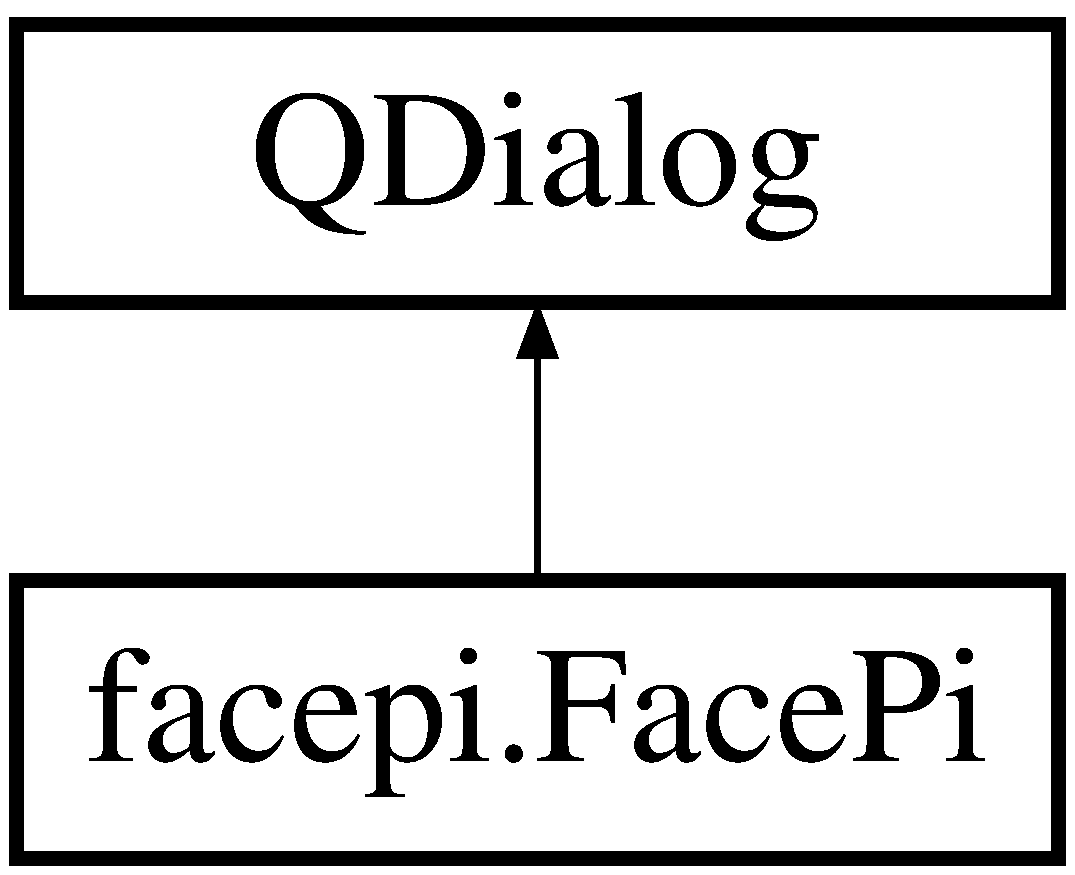
\includegraphics[height=2.000000cm]{classfacepi_1_1_face_pi}
\end{center}
\end{figure}
\subsection*{Métodos públicos}
\begin{DoxyCompactItemize}
\item 
def \mbox{\hyperlink{classfacepi_1_1_face_pi_a68ec1ba24536fdb7cc03bc0b6f7a2bee}{\+\_\+\+\_\+init\+\_\+\+\_\+}} (self)
\begin{DoxyCompactList}\small\item\em Contructor. \end{DoxyCompactList}\item 
def \mbox{\hyperlink{classfacepi_1_1_face_pi_ad558e4b8c0cf5a01e4eb8ea7aad5cd77}{init\+UI}} (self)
\begin{DoxyCompactList}\small\item\em Genera el interfaz grafico. \end{DoxyCompactList}\item 
def \mbox{\hyperlink{classfacepi_1_1_face_pi_a18271336c0cf8270a1f1a50acb4b4953}{create\+Grid\+Layout}} (self)
\begin{DoxyCompactList}\small\item\em Crea la disposicion de objetos en gradilla. \end{DoxyCompactList}\item 
def \mbox{\hyperlink{classfacepi_1_1_face_pi_a966fe4796c56e70b656ccd92df60cbb9}{read\+Config}} (self, \mbox{\hyperlink{classfacepi_1_1_face_pi_a49127c31ef994508911027e13dada2ad}{ini\+File}})
\begin{DoxyCompactList}\small\item\em Lee la configuracion del sistema. \end{DoxyCompactList}\item 
def \mbox{\hyperlink{classfacepi_1_1_face_pi_ae6fb3ad150c4edf520d7a6e438af4cd8}{save\+Config}} (self, \mbox{\hyperlink{classfacepi_1_1_face_pi_a49127c31ef994508911027e13dada2ad}{ini\+File}})
\begin{DoxyCompactList}\small\item\em Salva la configuracion al archivo de configuracion. \end{DoxyCompactList}\item 
def \mbox{\hyperlink{classfacepi_1_1_face_pi_a6ef1408ba24ad470f358594e60b9a85a}{config\+App}} (self)
\begin{DoxyCompactList}\small\item\em Carga los dialogos de configuracion y salva los parametros. \end{DoxyCompactList}\item 
def \mbox{\hyperlink{classfacepi_1_1_face_pi_af0325d200c0071bffaa042c128b5abac}{get\+Key}} (self)
\begin{DoxyCompactList}\small\item\em Dialogo para solicitud de clave. \end{DoxyCompactList}\item 
def \mbox{\hyperlink{classfacepi_1_1_face_pi_a15ff7fa69bb7b967444a659fdb66f7b9}{get\+Server}} (self)
\begin{DoxyCompactList}\small\item\em Dialogo para solicitud de servidor. \end{DoxyCompactList}\item 
def \mbox{\hyperlink{classfacepi_1_1_face_pi_a399f4c1740f88e9b742051a8d2332f55}{get\+Group}} (self)
\begin{DoxyCompactList}\small\item\em Dialogo para solicitud de grupo. \end{DoxyCompactList}\item 
def \mbox{\hyperlink{classfacepi_1_1_face_pi_ac7c8594736211d56756975342d24934f}{get\+Timestamp}} (self)
\begin{DoxyCompactList}\small\item\em Lee el puerto de serie Bluetooth. \end{DoxyCompactList}\item 
def \mbox{\hyperlink{classfacepi_1_1_face_pi_aa6a20d44bd85ecbf4aaa6390707e9ffe}{capture}} (self)
\begin{DoxyCompactList}\small\item\em Captura una imagen. \end{DoxyCompactList}\item 
def \mbox{\hyperlink{classfacepi_1_1_face_pi_aabccf277e0113ec07ab30d74fbbf261e}{identify}} (self)
\begin{DoxyCompactList}\small\item\em Identifica rostros. \end{DoxyCompactList}\item 
def \mbox{\hyperlink{classfacepi_1_1_face_pi_ac94b516a6dd221032d2ec103f8af3242}{printC}} (self, text)
\begin{DoxyCompactList}\small\item\em Escribe un mensaje en la consola. \end{DoxyCompactList}\item 
def \mbox{\hyperlink{classfacepi_1_1_face_pi_a8e4d19c4f06839b99a061844243668bd}{clearC}} (self)
\begin{DoxyCompactList}\small\item\em Limpia la consola. \end{DoxyCompactList}\item 
def \mbox{\hyperlink{classfacepi_1_1_face_pi_a32fcd9ee614d028b3722a0a18f07d03d}{alert\+Dialog}} (self, msg)
\begin{DoxyCompactList}\small\item\em Genera un cuadro de alerta. \end{DoxyCompactList}\item 
def \mbox{\hyperlink{classfacepi_1_1_face_pi_a28d7a48a53a13bfc501f3ee1de5e1968}{save\+Image}} (self)
\begin{DoxyCompactList}\small\item\em Salva la imagen mediante cuadro de seleccion de archivos. \end{DoxyCompactList}\item 
def \mbox{\hyperlink{classfacepi_1_1_face_pi_acaaf24b558c23d9c2831cbfc67e1fed7}{load\+Image}} (self)
\begin{DoxyCompactList}\small\item\em Carga imagen mediante cuadro de seleccion de archivos. \end{DoxyCompactList}\item 
def \mbox{\hyperlink{classfacepi_1_1_face_pi_a69e8a3b9b7df0e5b6fc00233debe46a7}{app\+Exit}} (self)
\begin{DoxyCompactList}\small\item\em Gestiona el cierre de la aplicacion. \end{DoxyCompactList}\end{DoxyCompactItemize}
\subsection*{Atributos públicos}
\begin{DoxyCompactItemize}
\item 
\mbox{\hyperlink{classfacepi_1_1_face_pi_afccfe61a4761c5a45b4fbc820a5240df}{title}}
\begin{DoxyCompactList}\small\item\em titulo de la aplicacion \end{DoxyCompactList}\item 
\mbox{\hyperlink{classfacepi_1_1_face_pi_a5a300c103ace38df66904b7be129fab4}{left}}
\begin{DoxyCompactList}\small\item\em Posicion izquierda de la aplicacion. \end{DoxyCompactList}\item 
\mbox{\hyperlink{classfacepi_1_1_face_pi_a187a0c2fb08f32d311610ba565e7887e}{top}}
\begin{DoxyCompactList}\small\item\em Posicion superior de la aplicacion. \end{DoxyCompactList}\item 
\mbox{\hyperlink{classfacepi_1_1_face_pi_a57e3ba2b24e564c5293372fd32408411}{width}}
\begin{DoxyCompactList}\small\item\em Ancho de la aplicacion. \end{DoxyCompactList}\item 
\mbox{\hyperlink{classfacepi_1_1_face_pi_a139e27fbb3d9131c28b1c0a18d0e5e82}{height}}
\begin{DoxyCompactList}\small\item\em Alto de la aplicacion. \end{DoxyCompactList}\item 
\mbox{\hyperlink{classfacepi_1_1_face_pi_a908848418be9c22c357748a0b3550869}{label}}
\begin{DoxyCompactList}\small\item\em Contenedor de objetos. \end{DoxyCompactList}\item 
\mbox{\hyperlink{classfacepi_1_1_face_pi_a10efba4963818e4ce358e3cc3580e223}{text\+Container}}
\begin{DoxyCompactList}\small\item\em Contenedor de texto de consola. \end{DoxyCompactList}\item 
\mbox{\hyperlink{classfacepi_1_1_face_pi_a265ba93b91b05aff63e24ffedbd8b488}{pixmap}}
\begin{DoxyCompactList}\small\item\em Contenedor de imagenes. \end{DoxyCompactList}\item 
\mbox{\hyperlink{classfacepi_1_1_face_pi_af8d79e94815c80b1ea8b98df8b5565f1}{camera}}
\begin{DoxyCompactList}\small\item\em Objeto de Pi\+Camera. \end{DoxyCompactList}\item 
\mbox{\hyperlink{classfacepi_1_1_face_pi_a4b3ecd462abe4ba265271f50c69a765a}{img}}
\begin{DoxyCompactList}\small\item\em Guarda la imagen mostrada en pantalla. \end{DoxyCompactList}\item 
\mbox{\hyperlink{classfacepi_1_1_face_pi_a49127c31ef994508911027e13dada2ad}{ini\+File}}
\begin{DoxyCompactList}\small\item\em Archivo de configuracion. \end{DoxyCompactList}\item 
\mbox{\hyperlink{classfacepi_1_1_face_pi_a160c61487b4522e4915a76fddc307248}{font}}
\begin{DoxyCompactList}\small\item\em Fuente para el rotulado de caras. \end{DoxyCompactList}\item 
\mbox{\hyperlink{classfacepi_1_1_face_pi_a0d82f2516e0c5daae93625f34a05eab6}{config}}
\begin{DoxyCompactList}\small\item\em Objeto que contiene parametros de configuracion. \end{DoxyCompactList}\item 
\mbox{\hyperlink{classfacepi_1_1_face_pi_aec6ab9276df6b39fdcf1ac346c28877e}{face\+Detector}}
\begin{DoxyCompactList}\small\item\em Ubicacion del filtro Haar. \end{DoxyCompactList}\item 
\mbox{\hyperlink{classfacepi_1_1_face_pi_a18d1b929c5d12dbea45397938fb65e31}{s\+Key}}
\begin{DoxyCompactList}\small\item\em Clave de suscripcion de Azure. \end{DoxyCompactList}\item 
\mbox{\hyperlink{classfacepi_1_1_face_pi_a873ed179b2f11752b2105b6926469a48}{server}}
\begin{DoxyCompactList}\small\item\em Servidor de Azure. \end{DoxyCompactList}\item 
\mbox{\hyperlink{classfacepi_1_1_face_pi_a8b55286218a2ba8914171c238f09c7bf}{group\+Name}}
\begin{DoxyCompactList}\small\item\em Grupo de personas de Azure. \end{DoxyCompactList}\item 
\mbox{\hyperlink{classfacepi_1_1_face_pi_a3ca8ad773fedc3dbd86653f4e32e46e9}{wait\+Time}}
\begin{DoxyCompactList}\small\item\em Tiempo de espera. \end{DoxyCompactList}\item 
\mbox{\hyperlink{classfacepi_1_1_face_pi_a3683c8fce62f0046f757d1c8dead6e7b}{recon\+Btn}}
\begin{DoxyCompactList}\small\item\em Boton de reconocimiento. \end{DoxyCompactList}\item 
\mbox{\hyperlink{classfacepi_1_1_face_pi_a14bf82467b2999f4bb10db0c5cf91449}{horizontal\+Group\+Box}}
\end{DoxyCompactItemize}


\subsection{Descripción detallada}
Clase principal de \mbox{\hyperlink{classfacepi_1_1_face_pi}{Face\+Pi}}. 

Genera el G\+UI y contiene funciones para la gestion del interfaz. Contiene funciones para la identificacion de rostros mediante captura o carga de imagenes 

\subsection{Documentación del constructor y destructor}
\mbox{\Hypertarget{classfacepi_1_1_face_pi_a68ec1ba24536fdb7cc03bc0b6f7a2bee}\label{classfacepi_1_1_face_pi_a68ec1ba24536fdb7cc03bc0b6f7a2bee}} 
\index{facepi\+::\+Face\+Pi@{facepi\+::\+Face\+Pi}!\+\_\+\+\_\+init\+\_\+\+\_\+@{\+\_\+\+\_\+init\+\_\+\+\_\+}}
\index{\+\_\+\+\_\+init\+\_\+\+\_\+@{\+\_\+\+\_\+init\+\_\+\+\_\+}!facepi\+::\+Face\+Pi@{facepi\+::\+Face\+Pi}}
\subsubsection{\texorpdfstring{\+\_\+\+\_\+init\+\_\+\+\_\+()}{\_\_init\_\_()}}
{\footnotesize\ttfamily def facepi.\+Face\+Pi.\+\_\+\+\_\+init\+\_\+\+\_\+ (\begin{DoxyParamCaption}\item[{}]{self }\end{DoxyParamCaption})}



Contructor. 



\subsection{Documentación de las funciones miembro}
\mbox{\Hypertarget{classfacepi_1_1_face_pi_a32fcd9ee614d028b3722a0a18f07d03d}\label{classfacepi_1_1_face_pi_a32fcd9ee614d028b3722a0a18f07d03d}} 
\index{facepi\+::\+Face\+Pi@{facepi\+::\+Face\+Pi}!alert\+Dialog@{alert\+Dialog}}
\index{alert\+Dialog@{alert\+Dialog}!facepi\+::\+Face\+Pi@{facepi\+::\+Face\+Pi}}
\subsubsection{\texorpdfstring{alert\+Dialog()}{alertDialog()}}
{\footnotesize\ttfamily def facepi.\+Face\+Pi.\+alert\+Dialog (\begin{DoxyParamCaption}\item[{}]{self,  }\item[{}]{msg }\end{DoxyParamCaption})}



Genera un cuadro de alerta. 


\begin{DoxyParams}{Parámetros}
{\em msg} & Texto del mensaje de alerta \\
\hline
\end{DoxyParams}
\mbox{\Hypertarget{classfacepi_1_1_face_pi_a69e8a3b9b7df0e5b6fc00233debe46a7}\label{classfacepi_1_1_face_pi_a69e8a3b9b7df0e5b6fc00233debe46a7}} 
\index{facepi\+::\+Face\+Pi@{facepi\+::\+Face\+Pi}!app\+Exit@{app\+Exit}}
\index{app\+Exit@{app\+Exit}!facepi\+::\+Face\+Pi@{facepi\+::\+Face\+Pi}}
\subsubsection{\texorpdfstring{app\+Exit()}{appExit()}}
{\footnotesize\ttfamily def facepi.\+Face\+Pi.\+app\+Exit (\begin{DoxyParamCaption}\item[{}]{self }\end{DoxyParamCaption})}



Gestiona el cierre de la aplicacion. 

\mbox{\Hypertarget{classfacepi_1_1_face_pi_aa6a20d44bd85ecbf4aaa6390707e9ffe}\label{classfacepi_1_1_face_pi_aa6a20d44bd85ecbf4aaa6390707e9ffe}} 
\index{facepi\+::\+Face\+Pi@{facepi\+::\+Face\+Pi}!capture@{capture}}
\index{capture@{capture}!facepi\+::\+Face\+Pi@{facepi\+::\+Face\+Pi}}
\subsubsection{\texorpdfstring{capture()}{capture()}}
{\footnotesize\ttfamily def facepi.\+Face\+Pi.\+capture (\begin{DoxyParamCaption}\item[{}]{self }\end{DoxyParamCaption})}



Captura una imagen. 

\mbox{\Hypertarget{classfacepi_1_1_face_pi_a8e4d19c4f06839b99a061844243668bd}\label{classfacepi_1_1_face_pi_a8e4d19c4f06839b99a061844243668bd}} 
\index{facepi\+::\+Face\+Pi@{facepi\+::\+Face\+Pi}!clearC@{clearC}}
\index{clearC@{clearC}!facepi\+::\+Face\+Pi@{facepi\+::\+Face\+Pi}}
\subsubsection{\texorpdfstring{clear\+C()}{clearC()}}
{\footnotesize\ttfamily def facepi.\+Face\+Pi.\+clearC (\begin{DoxyParamCaption}\item[{}]{self }\end{DoxyParamCaption})}



Limpia la consola. 

\mbox{\Hypertarget{classfacepi_1_1_face_pi_a6ef1408ba24ad470f358594e60b9a85a}\label{classfacepi_1_1_face_pi_a6ef1408ba24ad470f358594e60b9a85a}} 
\index{facepi\+::\+Face\+Pi@{facepi\+::\+Face\+Pi}!config\+App@{config\+App}}
\index{config\+App@{config\+App}!facepi\+::\+Face\+Pi@{facepi\+::\+Face\+Pi}}
\subsubsection{\texorpdfstring{config\+App()}{configApp()}}
{\footnotesize\ttfamily def facepi.\+Face\+Pi.\+config\+App (\begin{DoxyParamCaption}\item[{}]{self }\end{DoxyParamCaption})}



Carga los dialogos de configuracion y salva los parametros. 

\mbox{\Hypertarget{classfacepi_1_1_face_pi_a18271336c0cf8270a1f1a50acb4b4953}\label{classfacepi_1_1_face_pi_a18271336c0cf8270a1f1a50acb4b4953}} 
\index{facepi\+::\+Face\+Pi@{facepi\+::\+Face\+Pi}!create\+Grid\+Layout@{create\+Grid\+Layout}}
\index{create\+Grid\+Layout@{create\+Grid\+Layout}!facepi\+::\+Face\+Pi@{facepi\+::\+Face\+Pi}}
\subsubsection{\texorpdfstring{create\+Grid\+Layout()}{createGridLayout()}}
{\footnotesize\ttfamily def facepi.\+Face\+Pi.\+create\+Grid\+Layout (\begin{DoxyParamCaption}\item[{}]{self }\end{DoxyParamCaption})}



Crea la disposicion de objetos en gradilla. 

\mbox{\Hypertarget{classfacepi_1_1_face_pi_a399f4c1740f88e9b742051a8d2332f55}\label{classfacepi_1_1_face_pi_a399f4c1740f88e9b742051a8d2332f55}} 
\index{facepi\+::\+Face\+Pi@{facepi\+::\+Face\+Pi}!get\+Group@{get\+Group}}
\index{get\+Group@{get\+Group}!facepi\+::\+Face\+Pi@{facepi\+::\+Face\+Pi}}
\subsubsection{\texorpdfstring{get\+Group()}{getGroup()}}
{\footnotesize\ttfamily def facepi.\+Face\+Pi.\+get\+Group (\begin{DoxyParamCaption}\item[{}]{self }\end{DoxyParamCaption})}



Dialogo para solicitud de grupo. 

\mbox{\Hypertarget{classfacepi_1_1_face_pi_af0325d200c0071bffaa042c128b5abac}\label{classfacepi_1_1_face_pi_af0325d200c0071bffaa042c128b5abac}} 
\index{facepi\+::\+Face\+Pi@{facepi\+::\+Face\+Pi}!get\+Key@{get\+Key}}
\index{get\+Key@{get\+Key}!facepi\+::\+Face\+Pi@{facepi\+::\+Face\+Pi}}
\subsubsection{\texorpdfstring{get\+Key()}{getKey()}}
{\footnotesize\ttfamily def facepi.\+Face\+Pi.\+get\+Key (\begin{DoxyParamCaption}\item[{}]{self }\end{DoxyParamCaption})}



Dialogo para solicitud de clave. 

\mbox{\Hypertarget{classfacepi_1_1_face_pi_a15ff7fa69bb7b967444a659fdb66f7b9}\label{classfacepi_1_1_face_pi_a15ff7fa69bb7b967444a659fdb66f7b9}} 
\index{facepi\+::\+Face\+Pi@{facepi\+::\+Face\+Pi}!get\+Server@{get\+Server}}
\index{get\+Server@{get\+Server}!facepi\+::\+Face\+Pi@{facepi\+::\+Face\+Pi}}
\subsubsection{\texorpdfstring{get\+Server()}{getServer()}}
{\footnotesize\ttfamily def facepi.\+Face\+Pi.\+get\+Server (\begin{DoxyParamCaption}\item[{}]{self }\end{DoxyParamCaption})}



Dialogo para solicitud de servidor. 

\mbox{\Hypertarget{classfacepi_1_1_face_pi_ac7c8594736211d56756975342d24934f}\label{classfacepi_1_1_face_pi_ac7c8594736211d56756975342d24934f}} 
\index{facepi\+::\+Face\+Pi@{facepi\+::\+Face\+Pi}!get\+Timestamp@{get\+Timestamp}}
\index{get\+Timestamp@{get\+Timestamp}!facepi\+::\+Face\+Pi@{facepi\+::\+Face\+Pi}}
\subsubsection{\texorpdfstring{get\+Timestamp()}{getTimestamp()}}
{\footnotesize\ttfamily def facepi.\+Face\+Pi.\+get\+Timestamp (\begin{DoxyParamCaption}\item[{}]{self }\end{DoxyParamCaption})}



Lee el puerto de serie Bluetooth. 

\begin{DoxyReturn}{Devuelve}
now\+Str String con la marca temporal. 
\end{DoxyReturn}
\mbox{\Hypertarget{classfacepi_1_1_face_pi_aabccf277e0113ec07ab30d74fbbf261e}\label{classfacepi_1_1_face_pi_aabccf277e0113ec07ab30d74fbbf261e}} 
\index{facepi\+::\+Face\+Pi@{facepi\+::\+Face\+Pi}!identify@{identify}}
\index{identify@{identify}!facepi\+::\+Face\+Pi@{facepi\+::\+Face\+Pi}}
\subsubsection{\texorpdfstring{identify()}{identify()}}
{\footnotesize\ttfamily def facepi.\+Face\+Pi.\+identify (\begin{DoxyParamCaption}\item[{}]{self }\end{DoxyParamCaption})}



Identifica rostros. 

\mbox{\Hypertarget{classfacepi_1_1_face_pi_ad558e4b8c0cf5a01e4eb8ea7aad5cd77}\label{classfacepi_1_1_face_pi_ad558e4b8c0cf5a01e4eb8ea7aad5cd77}} 
\index{facepi\+::\+Face\+Pi@{facepi\+::\+Face\+Pi}!init\+UI@{init\+UI}}
\index{init\+UI@{init\+UI}!facepi\+::\+Face\+Pi@{facepi\+::\+Face\+Pi}}
\subsubsection{\texorpdfstring{init\+U\+I()}{initUI()}}
{\footnotesize\ttfamily def facepi.\+Face\+Pi.\+init\+UI (\begin{DoxyParamCaption}\item[{}]{self }\end{DoxyParamCaption})}



Genera el interfaz grafico. 

\mbox{\Hypertarget{classfacepi_1_1_face_pi_acaaf24b558c23d9c2831cbfc67e1fed7}\label{classfacepi_1_1_face_pi_acaaf24b558c23d9c2831cbfc67e1fed7}} 
\index{facepi\+::\+Face\+Pi@{facepi\+::\+Face\+Pi}!load\+Image@{load\+Image}}
\index{load\+Image@{load\+Image}!facepi\+::\+Face\+Pi@{facepi\+::\+Face\+Pi}}
\subsubsection{\texorpdfstring{load\+Image()}{loadImage()}}
{\footnotesize\ttfamily def facepi.\+Face\+Pi.\+load\+Image (\begin{DoxyParamCaption}\item[{}]{self }\end{DoxyParamCaption})}



Carga imagen mediante cuadro de seleccion de archivos. 

\mbox{\Hypertarget{classfacepi_1_1_face_pi_ac94b516a6dd221032d2ec103f8af3242}\label{classfacepi_1_1_face_pi_ac94b516a6dd221032d2ec103f8af3242}} 
\index{facepi\+::\+Face\+Pi@{facepi\+::\+Face\+Pi}!printC@{printC}}
\index{printC@{printC}!facepi\+::\+Face\+Pi@{facepi\+::\+Face\+Pi}}
\subsubsection{\texorpdfstring{print\+C()}{printC()}}
{\footnotesize\ttfamily def facepi.\+Face\+Pi.\+printC (\begin{DoxyParamCaption}\item[{}]{self,  }\item[{}]{text }\end{DoxyParamCaption})}



Escribe un mensaje en la consola. 


\begin{DoxyParams}{Parámetros}
{\em text} & \\
\hline
\end{DoxyParams}
\mbox{\Hypertarget{classfacepi_1_1_face_pi_a966fe4796c56e70b656ccd92df60cbb9}\label{classfacepi_1_1_face_pi_a966fe4796c56e70b656ccd92df60cbb9}} 
\index{facepi\+::\+Face\+Pi@{facepi\+::\+Face\+Pi}!read\+Config@{read\+Config}}
\index{read\+Config@{read\+Config}!facepi\+::\+Face\+Pi@{facepi\+::\+Face\+Pi}}
\subsubsection{\texorpdfstring{read\+Config()}{readConfig()}}
{\footnotesize\ttfamily def facepi.\+Face\+Pi.\+read\+Config (\begin{DoxyParamCaption}\item[{}]{self,  }\item[{}]{ini\+File }\end{DoxyParamCaption})}



Lee la configuracion del sistema. 


\begin{DoxyParams}{Parámetros}
{\em ini\+File} & Archivo de configuracion \\
\hline
\end{DoxyParams}
\mbox{\Hypertarget{classfacepi_1_1_face_pi_ae6fb3ad150c4edf520d7a6e438af4cd8}\label{classfacepi_1_1_face_pi_ae6fb3ad150c4edf520d7a6e438af4cd8}} 
\index{facepi\+::\+Face\+Pi@{facepi\+::\+Face\+Pi}!save\+Config@{save\+Config}}
\index{save\+Config@{save\+Config}!facepi\+::\+Face\+Pi@{facepi\+::\+Face\+Pi}}
\subsubsection{\texorpdfstring{save\+Config()}{saveConfig()}}
{\footnotesize\ttfamily def facepi.\+Face\+Pi.\+save\+Config (\begin{DoxyParamCaption}\item[{}]{self,  }\item[{}]{ini\+File }\end{DoxyParamCaption})}



Salva la configuracion al archivo de configuracion. 


\begin{DoxyParams}{Parámetros}
{\em ini\+File} & Archivo de configuracion \\
\hline
\end{DoxyParams}
\mbox{\Hypertarget{classfacepi_1_1_face_pi_a28d7a48a53a13bfc501f3ee1de5e1968}\label{classfacepi_1_1_face_pi_a28d7a48a53a13bfc501f3ee1de5e1968}} 
\index{facepi\+::\+Face\+Pi@{facepi\+::\+Face\+Pi}!save\+Image@{save\+Image}}
\index{save\+Image@{save\+Image}!facepi\+::\+Face\+Pi@{facepi\+::\+Face\+Pi}}
\subsubsection{\texorpdfstring{save\+Image()}{saveImage()}}
{\footnotesize\ttfamily def facepi.\+Face\+Pi.\+save\+Image (\begin{DoxyParamCaption}\item[{}]{self }\end{DoxyParamCaption})}



Salva la imagen mediante cuadro de seleccion de archivos. 



\subsection{Documentación de los datos miembro}
\mbox{\Hypertarget{classfacepi_1_1_face_pi_af8d79e94815c80b1ea8b98df8b5565f1}\label{classfacepi_1_1_face_pi_af8d79e94815c80b1ea8b98df8b5565f1}} 
\index{facepi\+::\+Face\+Pi@{facepi\+::\+Face\+Pi}!camera@{camera}}
\index{camera@{camera}!facepi\+::\+Face\+Pi@{facepi\+::\+Face\+Pi}}
\subsubsection{\texorpdfstring{camera}{camera}}
{\footnotesize\ttfamily facepi.\+Face\+Pi.\+camera}



Objeto de Pi\+Camera. 

\mbox{\Hypertarget{classfacepi_1_1_face_pi_a0d82f2516e0c5daae93625f34a05eab6}\label{classfacepi_1_1_face_pi_a0d82f2516e0c5daae93625f34a05eab6}} 
\index{facepi\+::\+Face\+Pi@{facepi\+::\+Face\+Pi}!config@{config}}
\index{config@{config}!facepi\+::\+Face\+Pi@{facepi\+::\+Face\+Pi}}
\subsubsection{\texorpdfstring{config}{config}}
{\footnotesize\ttfamily facepi.\+Face\+Pi.\+config}



Objeto que contiene parametros de configuracion. 

\mbox{\Hypertarget{classfacepi_1_1_face_pi_aec6ab9276df6b39fdcf1ac346c28877e}\label{classfacepi_1_1_face_pi_aec6ab9276df6b39fdcf1ac346c28877e}} 
\index{facepi\+::\+Face\+Pi@{facepi\+::\+Face\+Pi}!face\+Detector@{face\+Detector}}
\index{face\+Detector@{face\+Detector}!facepi\+::\+Face\+Pi@{facepi\+::\+Face\+Pi}}
\subsubsection{\texorpdfstring{face\+Detector}{faceDetector}}
{\footnotesize\ttfamily facepi.\+Face\+Pi.\+face\+Detector}



Ubicacion del filtro Haar. 

\mbox{\Hypertarget{classfacepi_1_1_face_pi_a160c61487b4522e4915a76fddc307248}\label{classfacepi_1_1_face_pi_a160c61487b4522e4915a76fddc307248}} 
\index{facepi\+::\+Face\+Pi@{facepi\+::\+Face\+Pi}!font@{font}}
\index{font@{font}!facepi\+::\+Face\+Pi@{facepi\+::\+Face\+Pi}}
\subsubsection{\texorpdfstring{font}{font}}
{\footnotesize\ttfamily facepi.\+Face\+Pi.\+font}



Fuente para el rotulado de caras. 

\mbox{\Hypertarget{classfacepi_1_1_face_pi_a8b55286218a2ba8914171c238f09c7bf}\label{classfacepi_1_1_face_pi_a8b55286218a2ba8914171c238f09c7bf}} 
\index{facepi\+::\+Face\+Pi@{facepi\+::\+Face\+Pi}!group\+Name@{group\+Name}}
\index{group\+Name@{group\+Name}!facepi\+::\+Face\+Pi@{facepi\+::\+Face\+Pi}}
\subsubsection{\texorpdfstring{group\+Name}{groupName}}
{\footnotesize\ttfamily facepi.\+Face\+Pi.\+group\+Name}



Grupo de personas de Azure. 

\mbox{\Hypertarget{classfacepi_1_1_face_pi_a139e27fbb3d9131c28b1c0a18d0e5e82}\label{classfacepi_1_1_face_pi_a139e27fbb3d9131c28b1c0a18d0e5e82}} 
\index{facepi\+::\+Face\+Pi@{facepi\+::\+Face\+Pi}!height@{height}}
\index{height@{height}!facepi\+::\+Face\+Pi@{facepi\+::\+Face\+Pi}}
\subsubsection{\texorpdfstring{height}{height}}
{\footnotesize\ttfamily facepi.\+Face\+Pi.\+height}



Alto de la aplicacion. 

\mbox{\Hypertarget{classfacepi_1_1_face_pi_a14bf82467b2999f4bb10db0c5cf91449}\label{classfacepi_1_1_face_pi_a14bf82467b2999f4bb10db0c5cf91449}} 
\index{facepi\+::\+Face\+Pi@{facepi\+::\+Face\+Pi}!horizontal\+Group\+Box@{horizontal\+Group\+Box}}
\index{horizontal\+Group\+Box@{horizontal\+Group\+Box}!facepi\+::\+Face\+Pi@{facepi\+::\+Face\+Pi}}
\subsubsection{\texorpdfstring{horizontal\+Group\+Box}{horizontalGroupBox}}
{\footnotesize\ttfamily facepi.\+Face\+Pi.\+horizontal\+Group\+Box}

\mbox{\Hypertarget{classfacepi_1_1_face_pi_a4b3ecd462abe4ba265271f50c69a765a}\label{classfacepi_1_1_face_pi_a4b3ecd462abe4ba265271f50c69a765a}} 
\index{facepi\+::\+Face\+Pi@{facepi\+::\+Face\+Pi}!img@{img}}
\index{img@{img}!facepi\+::\+Face\+Pi@{facepi\+::\+Face\+Pi}}
\subsubsection{\texorpdfstring{img}{img}}
{\footnotesize\ttfamily facepi.\+Face\+Pi.\+img}



Guarda la imagen mostrada en pantalla. 

\mbox{\Hypertarget{classfacepi_1_1_face_pi_a49127c31ef994508911027e13dada2ad}\label{classfacepi_1_1_face_pi_a49127c31ef994508911027e13dada2ad}} 
\index{facepi\+::\+Face\+Pi@{facepi\+::\+Face\+Pi}!ini\+File@{ini\+File}}
\index{ini\+File@{ini\+File}!facepi\+::\+Face\+Pi@{facepi\+::\+Face\+Pi}}
\subsubsection{\texorpdfstring{ini\+File}{iniFile}}
{\footnotesize\ttfamily facepi.\+Face\+Pi.\+ini\+File}



Archivo de configuracion. 

\mbox{\Hypertarget{classfacepi_1_1_face_pi_a908848418be9c22c357748a0b3550869}\label{classfacepi_1_1_face_pi_a908848418be9c22c357748a0b3550869}} 
\index{facepi\+::\+Face\+Pi@{facepi\+::\+Face\+Pi}!label@{label}}
\index{label@{label}!facepi\+::\+Face\+Pi@{facepi\+::\+Face\+Pi}}
\subsubsection{\texorpdfstring{label}{label}}
{\footnotesize\ttfamily facepi.\+Face\+Pi.\+label}



Contenedor de objetos. 

\mbox{\Hypertarget{classfacepi_1_1_face_pi_a5a300c103ace38df66904b7be129fab4}\label{classfacepi_1_1_face_pi_a5a300c103ace38df66904b7be129fab4}} 
\index{facepi\+::\+Face\+Pi@{facepi\+::\+Face\+Pi}!left@{left}}
\index{left@{left}!facepi\+::\+Face\+Pi@{facepi\+::\+Face\+Pi}}
\subsubsection{\texorpdfstring{left}{left}}
{\footnotesize\ttfamily facepi.\+Face\+Pi.\+left}



Posicion izquierda de la aplicacion. 

\mbox{\Hypertarget{classfacepi_1_1_face_pi_a265ba93b91b05aff63e24ffedbd8b488}\label{classfacepi_1_1_face_pi_a265ba93b91b05aff63e24ffedbd8b488}} 
\index{facepi\+::\+Face\+Pi@{facepi\+::\+Face\+Pi}!pixmap@{pixmap}}
\index{pixmap@{pixmap}!facepi\+::\+Face\+Pi@{facepi\+::\+Face\+Pi}}
\subsubsection{\texorpdfstring{pixmap}{pixmap}}
{\footnotesize\ttfamily facepi.\+Face\+Pi.\+pixmap}



Contenedor de imagenes. 

\mbox{\Hypertarget{classfacepi_1_1_face_pi_a3683c8fce62f0046f757d1c8dead6e7b}\label{classfacepi_1_1_face_pi_a3683c8fce62f0046f757d1c8dead6e7b}} 
\index{facepi\+::\+Face\+Pi@{facepi\+::\+Face\+Pi}!recon\+Btn@{recon\+Btn}}
\index{recon\+Btn@{recon\+Btn}!facepi\+::\+Face\+Pi@{facepi\+::\+Face\+Pi}}
\subsubsection{\texorpdfstring{recon\+Btn}{reconBtn}}
{\footnotesize\ttfamily facepi.\+Face\+Pi.\+recon\+Btn}



Boton de reconocimiento. 

\mbox{\Hypertarget{classfacepi_1_1_face_pi_a873ed179b2f11752b2105b6926469a48}\label{classfacepi_1_1_face_pi_a873ed179b2f11752b2105b6926469a48}} 
\index{facepi\+::\+Face\+Pi@{facepi\+::\+Face\+Pi}!server@{server}}
\index{server@{server}!facepi\+::\+Face\+Pi@{facepi\+::\+Face\+Pi}}
\subsubsection{\texorpdfstring{server}{server}}
{\footnotesize\ttfamily facepi.\+Face\+Pi.\+server}



Servidor de Azure. 

\mbox{\Hypertarget{classfacepi_1_1_face_pi_a18d1b929c5d12dbea45397938fb65e31}\label{classfacepi_1_1_face_pi_a18d1b929c5d12dbea45397938fb65e31}} 
\index{facepi\+::\+Face\+Pi@{facepi\+::\+Face\+Pi}!s\+Key@{s\+Key}}
\index{s\+Key@{s\+Key}!facepi\+::\+Face\+Pi@{facepi\+::\+Face\+Pi}}
\subsubsection{\texorpdfstring{s\+Key}{sKey}}
{\footnotesize\ttfamily facepi.\+Face\+Pi.\+s\+Key}



Clave de suscripcion de Azure. 

\mbox{\Hypertarget{classfacepi_1_1_face_pi_a10efba4963818e4ce358e3cc3580e223}\label{classfacepi_1_1_face_pi_a10efba4963818e4ce358e3cc3580e223}} 
\index{facepi\+::\+Face\+Pi@{facepi\+::\+Face\+Pi}!text\+Container@{text\+Container}}
\index{text\+Container@{text\+Container}!facepi\+::\+Face\+Pi@{facepi\+::\+Face\+Pi}}
\subsubsection{\texorpdfstring{text\+Container}{textContainer}}
{\footnotesize\ttfamily facepi.\+Face\+Pi.\+text\+Container}



Contenedor de texto de consola. 

\mbox{\Hypertarget{classfacepi_1_1_face_pi_afccfe61a4761c5a45b4fbc820a5240df}\label{classfacepi_1_1_face_pi_afccfe61a4761c5a45b4fbc820a5240df}} 
\index{facepi\+::\+Face\+Pi@{facepi\+::\+Face\+Pi}!title@{title}}
\index{title@{title}!facepi\+::\+Face\+Pi@{facepi\+::\+Face\+Pi}}
\subsubsection{\texorpdfstring{title}{title}}
{\footnotesize\ttfamily facepi.\+Face\+Pi.\+title}



titulo de la aplicacion 

\mbox{\Hypertarget{classfacepi_1_1_face_pi_a187a0c2fb08f32d311610ba565e7887e}\label{classfacepi_1_1_face_pi_a187a0c2fb08f32d311610ba565e7887e}} 
\index{facepi\+::\+Face\+Pi@{facepi\+::\+Face\+Pi}!top@{top}}
\index{top@{top}!facepi\+::\+Face\+Pi@{facepi\+::\+Face\+Pi}}
\subsubsection{\texorpdfstring{top}{top}}
{\footnotesize\ttfamily facepi.\+Face\+Pi.\+top}



Posicion superior de la aplicacion. 

\mbox{\Hypertarget{classfacepi_1_1_face_pi_a3ca8ad773fedc3dbd86653f4e32e46e9}\label{classfacepi_1_1_face_pi_a3ca8ad773fedc3dbd86653f4e32e46e9}} 
\index{facepi\+::\+Face\+Pi@{facepi\+::\+Face\+Pi}!wait\+Time@{wait\+Time}}
\index{wait\+Time@{wait\+Time}!facepi\+::\+Face\+Pi@{facepi\+::\+Face\+Pi}}
\subsubsection{\texorpdfstring{wait\+Time}{waitTime}}
{\footnotesize\ttfamily facepi.\+Face\+Pi.\+wait\+Time}



Tiempo de espera. 

\mbox{\Hypertarget{classfacepi_1_1_face_pi_a57e3ba2b24e564c5293372fd32408411}\label{classfacepi_1_1_face_pi_a57e3ba2b24e564c5293372fd32408411}} 
\index{facepi\+::\+Face\+Pi@{facepi\+::\+Face\+Pi}!width@{width}}
\index{width@{width}!facepi\+::\+Face\+Pi@{facepi\+::\+Face\+Pi}}
\subsubsection{\texorpdfstring{width}{width}}
{\footnotesize\ttfamily facepi.\+Face\+Pi.\+width}



Ancho de la aplicacion. 


\hypertarget{classcom_1_1loalon_1_1pfg_1_1facepal_1_1_global_class}{}\section{Referencia de la Clase com.\+loalon.\+pfg.\+facepal.\+Global\+Class}
\label{classcom_1_1loalon_1_1pfg_1_1facepal_1_1_global_class}\index{com.\+loalon.\+pfg.\+facepal.\+Global\+Class@{com.\+loalon.\+pfg.\+facepal.\+Global\+Class}}


Permite acceder de forma \char`\"{}global\char`\"{} al context de la aplicacion.  


Diagrama de herencias de com.\+loalon.\+pfg.\+facepal.\+Global\+Class\begin{figure}[H]
\begin{center}
\leavevmode
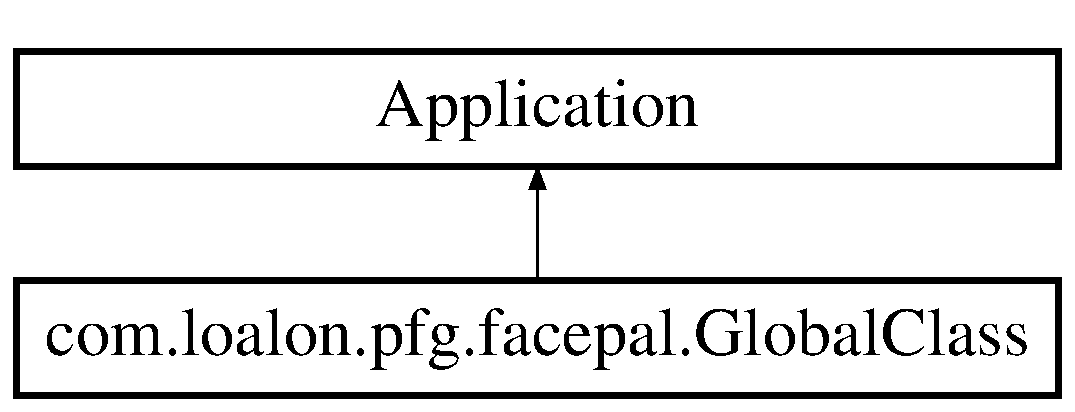
\includegraphics[height=2.000000cm]{classcom_1_1loalon_1_1pfg_1_1facepal_1_1_global_class}
\end{center}
\end{figure}
\subsection*{Métodos públicos}
\begin{DoxyCompactItemize}
\item 
void \mbox{\hyperlink{classcom_1_1loalon_1_1pfg_1_1facepal_1_1_global_class_ac9ef7a4e056cec00f0bd0db0beee5248}{on\+Create}} ()
\end{DoxyCompactItemize}
\subsection*{Atributos públicos estáticos}
\begin{DoxyCompactItemize}
\item 
static Context \mbox{\hyperlink{classcom_1_1loalon_1_1pfg_1_1facepal_1_1_global_class_a2c2206b0573eb16383ebd1bbe566faef}{context}}
\end{DoxyCompactItemize}


\subsection{Descripción detallada}
Permite acceder de forma \char`\"{}global\char`\"{} al context de la aplicacion. 

Created by Alonso on 05/04/2018. \begin{DoxyAuthor}{Autor}
Alonso Serrano 
\end{DoxyAuthor}
\begin{DoxyVersion}{Versión}
180405 
\end{DoxyVersion}


\subsection{Documentación de las funciones miembro}
\mbox{\Hypertarget{classcom_1_1loalon_1_1pfg_1_1facepal_1_1_global_class_ac9ef7a4e056cec00f0bd0db0beee5248}\label{classcom_1_1loalon_1_1pfg_1_1facepal_1_1_global_class_ac9ef7a4e056cec00f0bd0db0beee5248}} 
\index{com\+::loalon\+::pfg\+::facepal\+::\+Global\+Class@{com\+::loalon\+::pfg\+::facepal\+::\+Global\+Class}!on\+Create@{on\+Create}}
\index{on\+Create@{on\+Create}!com\+::loalon\+::pfg\+::facepal\+::\+Global\+Class@{com\+::loalon\+::pfg\+::facepal\+::\+Global\+Class}}
\subsubsection{\texorpdfstring{on\+Create()}{onCreate()}}
{\footnotesize\ttfamily void com.\+loalon.\+pfg.\+facepal.\+Global\+Class.\+on\+Create (\begin{DoxyParamCaption}{ }\end{DoxyParamCaption})}



\subsection{Documentación de los datos miembro}
\mbox{\Hypertarget{classcom_1_1loalon_1_1pfg_1_1facepal_1_1_global_class_a2c2206b0573eb16383ebd1bbe566faef}\label{classcom_1_1loalon_1_1pfg_1_1facepal_1_1_global_class_a2c2206b0573eb16383ebd1bbe566faef}} 
\index{com\+::loalon\+::pfg\+::facepal\+::\+Global\+Class@{com\+::loalon\+::pfg\+::facepal\+::\+Global\+Class}!context@{context}}
\index{context@{context}!com\+::loalon\+::pfg\+::facepal\+::\+Global\+Class@{com\+::loalon\+::pfg\+::facepal\+::\+Global\+Class}}
\subsubsection{\texorpdfstring{context}{context}}
{\footnotesize\ttfamily Context com.\+loalon.\+pfg.\+facepal.\+Global\+Class.\+context\hspace{0.3cm}{\ttfamily [static]}}


\hypertarget{classcom_1_1loalon_1_1pfg_1_1facepal_1_1_main_activity}{}\section{Referencia de la Clase com.\+loalon.\+pfg.\+facepal.\+Main\+Activity}
\label{classcom_1_1loalon_1_1pfg_1_1facepal_1_1_main_activity}\index{com.\+loalon.\+pfg.\+facepal.\+Main\+Activity@{com.\+loalon.\+pfg.\+facepal.\+Main\+Activity}}


Crea la actividad principal de Face\+Pal.  


Diagrama de herencias de com.\+loalon.\+pfg.\+facepal.\+Main\+Activity\begin{figure}[H]
\begin{center}
\leavevmode
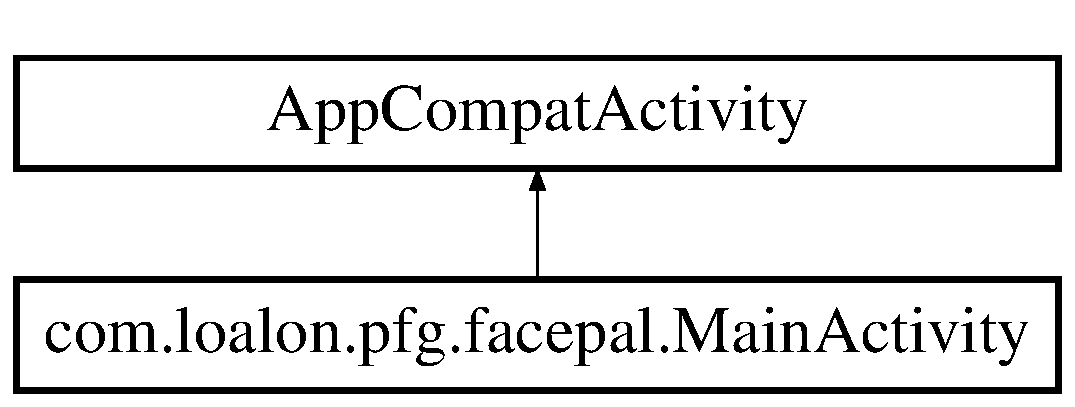
\includegraphics[height=2.000000cm]{classcom_1_1loalon_1_1pfg_1_1facepal_1_1_main_activity}
\end{center}
\end{figure}
\subsection*{Métodos públicos}
\begin{DoxyCompactItemize}
\item 
boolean \mbox{\hyperlink{classcom_1_1loalon_1_1pfg_1_1facepal_1_1_main_activity_a68c25a115ed9a0e16de384c85b1d7b16}{on\+Create\+Options\+Menu}} (Menu menu)
\item 
boolean \mbox{\hyperlink{classcom_1_1loalon_1_1pfg_1_1facepal_1_1_main_activity_ad5d4581e431dc5c30fb26698c79519a9}{on\+Options\+Item\+Selected}} (Menu\+Item item)
\end{DoxyCompactItemize}
\subsection*{Métodos protegidos}
\begin{DoxyCompactItemize}
\item 
void \mbox{\hyperlink{classcom_1_1loalon_1_1pfg_1_1facepal_1_1_main_activity_a2b74b94bc6860ee9c91f64af87c19042}{on\+Create}} (Bundle saved\+Instance\+State)
\item 
void \mbox{\hyperlink{classcom_1_1loalon_1_1pfg_1_1facepal_1_1_main_activity_ad39232d66aa75c28cee996ee6dc97df2}{on\+Activity\+Result}} (int request\+Code, int result\+Code, Intent data)
\end{DoxyCompactItemize}


\subsection{Descripción detallada}
Crea la actividad principal de Face\+Pal. 

Created by Alonso on 28/03/2018. \begin{DoxyAuthor}{Autor}
Alonso Serrano 
\end{DoxyAuthor}
\begin{DoxyVersion}{Versión}
180418 
\end{DoxyVersion}


\subsection{Documentación de las funciones miembro}
\mbox{\Hypertarget{classcom_1_1loalon_1_1pfg_1_1facepal_1_1_main_activity_ad39232d66aa75c28cee996ee6dc97df2}\label{classcom_1_1loalon_1_1pfg_1_1facepal_1_1_main_activity_ad39232d66aa75c28cee996ee6dc97df2}} 
\index{com\+::loalon\+::pfg\+::facepal\+::\+Main\+Activity@{com\+::loalon\+::pfg\+::facepal\+::\+Main\+Activity}!on\+Activity\+Result@{on\+Activity\+Result}}
\index{on\+Activity\+Result@{on\+Activity\+Result}!com\+::loalon\+::pfg\+::facepal\+::\+Main\+Activity@{com\+::loalon\+::pfg\+::facepal\+::\+Main\+Activity}}
\subsubsection{\texorpdfstring{on\+Activity\+Result()}{onActivityResult()}}
{\footnotesize\ttfamily void com.\+loalon.\+pfg.\+facepal.\+Main\+Activity.\+on\+Activity\+Result (\begin{DoxyParamCaption}\item[{int}]{request\+Code,  }\item[{int}]{result\+Code,  }\item[{Intent}]{data }\end{DoxyParamCaption})\hspace{0.3cm}{\ttfamily [protected]}}

\mbox{\Hypertarget{classcom_1_1loalon_1_1pfg_1_1facepal_1_1_main_activity_a2b74b94bc6860ee9c91f64af87c19042}\label{classcom_1_1loalon_1_1pfg_1_1facepal_1_1_main_activity_a2b74b94bc6860ee9c91f64af87c19042}} 
\index{com\+::loalon\+::pfg\+::facepal\+::\+Main\+Activity@{com\+::loalon\+::pfg\+::facepal\+::\+Main\+Activity}!on\+Create@{on\+Create}}
\index{on\+Create@{on\+Create}!com\+::loalon\+::pfg\+::facepal\+::\+Main\+Activity@{com\+::loalon\+::pfg\+::facepal\+::\+Main\+Activity}}
\subsubsection{\texorpdfstring{on\+Create()}{onCreate()}}
{\footnotesize\ttfamily void com.\+loalon.\+pfg.\+facepal.\+Main\+Activity.\+on\+Create (\begin{DoxyParamCaption}\item[{Bundle}]{saved\+Instance\+State }\end{DoxyParamCaption})\hspace{0.3cm}{\ttfamily [protected]}}

\mbox{\Hypertarget{classcom_1_1loalon_1_1pfg_1_1facepal_1_1_main_activity_a68c25a115ed9a0e16de384c85b1d7b16}\label{classcom_1_1loalon_1_1pfg_1_1facepal_1_1_main_activity_a68c25a115ed9a0e16de384c85b1d7b16}} 
\index{com\+::loalon\+::pfg\+::facepal\+::\+Main\+Activity@{com\+::loalon\+::pfg\+::facepal\+::\+Main\+Activity}!on\+Create\+Options\+Menu@{on\+Create\+Options\+Menu}}
\index{on\+Create\+Options\+Menu@{on\+Create\+Options\+Menu}!com\+::loalon\+::pfg\+::facepal\+::\+Main\+Activity@{com\+::loalon\+::pfg\+::facepal\+::\+Main\+Activity}}
\subsubsection{\texorpdfstring{on\+Create\+Options\+Menu()}{onCreateOptionsMenu()}}
{\footnotesize\ttfamily boolean com.\+loalon.\+pfg.\+facepal.\+Main\+Activity.\+on\+Create\+Options\+Menu (\begin{DoxyParamCaption}\item[{Menu}]{menu }\end{DoxyParamCaption})}

\mbox{\Hypertarget{classcom_1_1loalon_1_1pfg_1_1facepal_1_1_main_activity_ad5d4581e431dc5c30fb26698c79519a9}\label{classcom_1_1loalon_1_1pfg_1_1facepal_1_1_main_activity_ad5d4581e431dc5c30fb26698c79519a9}} 
\index{com\+::loalon\+::pfg\+::facepal\+::\+Main\+Activity@{com\+::loalon\+::pfg\+::facepal\+::\+Main\+Activity}!on\+Options\+Item\+Selected@{on\+Options\+Item\+Selected}}
\index{on\+Options\+Item\+Selected@{on\+Options\+Item\+Selected}!com\+::loalon\+::pfg\+::facepal\+::\+Main\+Activity@{com\+::loalon\+::pfg\+::facepal\+::\+Main\+Activity}}
\subsubsection{\texorpdfstring{on\+Options\+Item\+Selected()}{onOptionsItemSelected()}}
{\footnotesize\ttfamily boolean com.\+loalon.\+pfg.\+facepal.\+Main\+Activity.\+on\+Options\+Item\+Selected (\begin{DoxyParamCaption}\item[{Menu\+Item}]{item }\end{DoxyParamCaption})}


\hypertarget{classcom_1_1loalon_1_1pfg_1_1facepal_1_1_mini_snack}{}\section{Referencia de la Clase com.\+loalon.\+pfg.\+facepal.\+Mini\+Snack}
\label{classcom_1_1loalon_1_1pfg_1_1facepal_1_1_mini_snack}\index{com.\+loalon.\+pfg.\+facepal.\+Mini\+Snack@{com.\+loalon.\+pfg.\+facepal.\+Mini\+Snack}}


Crea objetos Snackbar con un duración indeterminada hasta que el usuario pulsa el boton OK El proposito de los Minisnacks es informar y que el usuario no realice otras acciones hasta comprender el mensaje que se le devuelve.  


\subsection*{Métodos públicos}
\begin{DoxyCompactItemize}
\item 
\mbox{\hyperlink{classcom_1_1loalon_1_1pfg_1_1facepal_1_1_mini_snack_a728b4a87e5b75c567711b17ac9da7192}{Mini\+Snack}} (View view, String text)
\end{DoxyCompactItemize}


\subsection{Descripción detallada}
Crea objetos Snackbar con un duración indeterminada hasta que el usuario pulsa el boton OK El proposito de los Minisnacks es informar y que el usuario no realice otras acciones hasta comprender el mensaje que se le devuelve. 

Created by Alonso on 09/04/2018. \begin{DoxyAuthor}{Autor}
Alonso Serrano 
\end{DoxyAuthor}
\begin{DoxyVersion}{Versión}
180409 
\end{DoxyVersion}


\subsection{Documentación del constructor y destructor}
\mbox{\Hypertarget{classcom_1_1loalon_1_1pfg_1_1facepal_1_1_mini_snack_a728b4a87e5b75c567711b17ac9da7192}\label{classcom_1_1loalon_1_1pfg_1_1facepal_1_1_mini_snack_a728b4a87e5b75c567711b17ac9da7192}} 
\index{com\+::loalon\+::pfg\+::facepal\+::\+Mini\+Snack@{com\+::loalon\+::pfg\+::facepal\+::\+Mini\+Snack}!Mini\+Snack@{Mini\+Snack}}
\index{Mini\+Snack@{Mini\+Snack}!com\+::loalon\+::pfg\+::facepal\+::\+Mini\+Snack@{com\+::loalon\+::pfg\+::facepal\+::\+Mini\+Snack}}
\subsubsection{\texorpdfstring{Mini\+Snack()}{MiniSnack()}}
{\footnotesize\ttfamily com.\+loalon.\+pfg.\+facepal.\+Mini\+Snack.\+Mini\+Snack (\begin{DoxyParamCaption}\item[{View}]{view,  }\item[{String}]{text }\end{DoxyParamCaption})}


\begin{DoxyParams}{Parámetros}
{\em view} & View donde se desea el mensaje \\
\hline
{\em text} & Texto que aparecera en el mensaje \\
\hline
\end{DoxyParams}

\hypertarget{classcom_1_1loalon_1_1pfg_1_1facepal_1_1_settings_activity}{}\section{Referencia de la Clase com.\+loalon.\+pfg.\+facepal.\+Settings\+Activity}
\label{classcom_1_1loalon_1_1pfg_1_1facepal_1_1_settings_activity}\index{com.\+loalon.\+pfg.\+facepal.\+Settings\+Activity@{com.\+loalon.\+pfg.\+facepal.\+Settings\+Activity}}


Creada por Android Studio para implementar el menu de configuración Esta clse contiene mas codigo del necesario, pero se mantiene para añadir mas opciones de configuracion en el futuro.  


Diagrama de herencias de com.\+loalon.\+pfg.\+facepal.\+Settings\+Activity\begin{figure}[H]
\begin{center}
\leavevmode
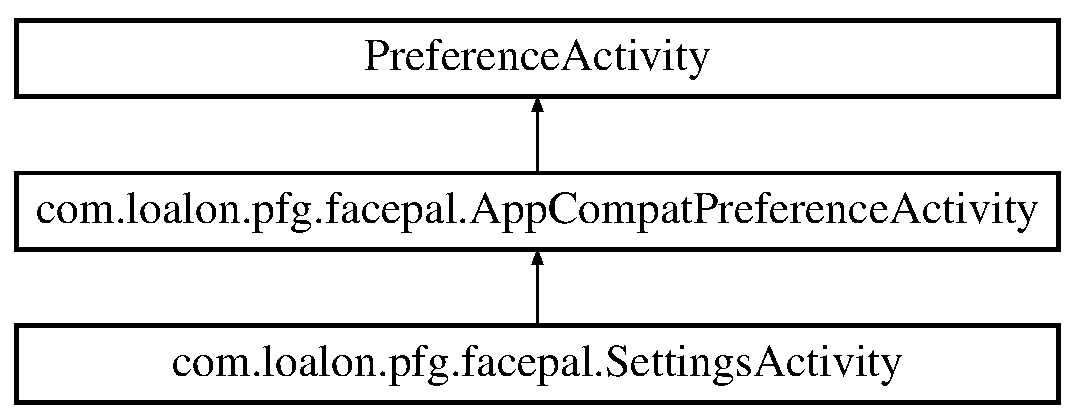
\includegraphics[height=3.000000cm]{classcom_1_1loalon_1_1pfg_1_1facepal_1_1_settings_activity}
\end{center}
\end{figure}
\subsection*{Clases}
\begin{DoxyCompactItemize}
\item 
class {\bfseries Data\+Sync\+Preference\+Fragment}
\begin{DoxyCompactList}\small\item\em This fragment shows data and sync preferences only. \end{DoxyCompactList}\item 
class {\bfseries General\+Preference\+Fragment}
\begin{DoxyCompactList}\small\item\em This fragment shows general preferences only. \end{DoxyCompactList}\item 
class {\bfseries Notification\+Preference\+Fragment}
\begin{DoxyCompactList}\small\item\em This fragment shows notification preferences only. \end{DoxyCompactList}\end{DoxyCompactItemize}
\subsection*{Métodos públicos}
\begin{DoxyCompactItemize}
\item 
boolean \mbox{\hyperlink{classcom_1_1loalon_1_1pfg_1_1facepal_1_1_settings_activity_a995efc7713ab73f011b94ca414978e2b}{on\+Is\+Multi\+Pane}} ()
\item 
void \mbox{\hyperlink{classcom_1_1loalon_1_1pfg_1_1facepal_1_1_settings_activity_a417499e165b77d2364d710513d2387d2}{on\+Build\+Headers}} (List$<$ Header $>$ target)
\end{DoxyCompactItemize}
\subsection*{Métodos protegidos}
\begin{DoxyCompactItemize}
\item 
void \mbox{\hyperlink{classcom_1_1loalon_1_1pfg_1_1facepal_1_1_settings_activity_acbf6db83f2e35289e4eafe26afeba7c5}{on\+Create}} (Bundle saved\+Instance\+State)
\item 
boolean \mbox{\hyperlink{classcom_1_1loalon_1_1pfg_1_1facepal_1_1_settings_activity_a98d18558ba2f0fd351970dbda2de05e8}{is\+Valid\+Fragment}} (String fragment\+Name)
\begin{DoxyCompactList}\small\item\em This method stops fragment injection in malicious applications. \end{DoxyCompactList}\end{DoxyCompactItemize}


\subsection{Descripción detallada}
Creada por Android Studio para implementar el menu de configuración Esta clse contiene mas codigo del necesario, pero se mantiene para añadir mas opciones de configuracion en el futuro. 

Created by Alonso on 28/03/2018. \begin{DoxyAuthor}{Autor}
Alonso Serrano 
\end{DoxyAuthor}
\begin{DoxyVersion}{Versión}
180331 A \mbox{\hyperlink{}{Preference\+Activity}} that presents a set of application settings. On handset devices, settings are presented as a single list. On tablets, settings are split by category, with category headers shown to the left of the list of settings. 
\end{DoxyVersion}
See \href{http://developer.android.com/design/patterns/settings.html}{\tt Android Design\+: Settings} for design guidelines and the \href{http://developer.android.com/guide/topics/ui/settings.html}{\tt Settings A\+PI Guide} for more information on developing a Settings UI. 

\subsection{Documentación de las funciones miembro}
\mbox{\Hypertarget{classcom_1_1loalon_1_1pfg_1_1facepal_1_1_settings_activity_a98d18558ba2f0fd351970dbda2de05e8}\label{classcom_1_1loalon_1_1pfg_1_1facepal_1_1_settings_activity_a98d18558ba2f0fd351970dbda2de05e8}} 
\index{com\+::loalon\+::pfg\+::facepal\+::\+Settings\+Activity@{com\+::loalon\+::pfg\+::facepal\+::\+Settings\+Activity}!is\+Valid\+Fragment@{is\+Valid\+Fragment}}
\index{is\+Valid\+Fragment@{is\+Valid\+Fragment}!com\+::loalon\+::pfg\+::facepal\+::\+Settings\+Activity@{com\+::loalon\+::pfg\+::facepal\+::\+Settings\+Activity}}
\subsubsection{\texorpdfstring{is\+Valid\+Fragment()}{isValidFragment()}}
{\footnotesize\ttfamily boolean com.\+loalon.\+pfg.\+facepal.\+Settings\+Activity.\+is\+Valid\+Fragment (\begin{DoxyParamCaption}\item[{String}]{fragment\+Name }\end{DoxyParamCaption})\hspace{0.3cm}{\ttfamily [protected]}}



This method stops fragment injection in malicious applications. 

Make sure to deny any unknown fragments here. \mbox{\Hypertarget{classcom_1_1loalon_1_1pfg_1_1facepal_1_1_settings_activity_a417499e165b77d2364d710513d2387d2}\label{classcom_1_1loalon_1_1pfg_1_1facepal_1_1_settings_activity_a417499e165b77d2364d710513d2387d2}} 
\index{com\+::loalon\+::pfg\+::facepal\+::\+Settings\+Activity@{com\+::loalon\+::pfg\+::facepal\+::\+Settings\+Activity}!on\+Build\+Headers@{on\+Build\+Headers}}
\index{on\+Build\+Headers@{on\+Build\+Headers}!com\+::loalon\+::pfg\+::facepal\+::\+Settings\+Activity@{com\+::loalon\+::pfg\+::facepal\+::\+Settings\+Activity}}
\subsubsection{\texorpdfstring{on\+Build\+Headers()}{onBuildHeaders()}}
{\footnotesize\ttfamily void com.\+loalon.\+pfg.\+facepal.\+Settings\+Activity.\+on\+Build\+Headers (\begin{DoxyParamCaption}\item[{List$<$ Header $>$}]{target }\end{DoxyParamCaption})}





\mbox{\Hypertarget{classcom_1_1loalon_1_1pfg_1_1facepal_1_1_settings_activity_acbf6db83f2e35289e4eafe26afeba7c5}\label{classcom_1_1loalon_1_1pfg_1_1facepal_1_1_settings_activity_acbf6db83f2e35289e4eafe26afeba7c5}} 
\index{com\+::loalon\+::pfg\+::facepal\+::\+Settings\+Activity@{com\+::loalon\+::pfg\+::facepal\+::\+Settings\+Activity}!on\+Create@{on\+Create}}
\index{on\+Create@{on\+Create}!com\+::loalon\+::pfg\+::facepal\+::\+Settings\+Activity@{com\+::loalon\+::pfg\+::facepal\+::\+Settings\+Activity}}
\subsubsection{\texorpdfstring{on\+Create()}{onCreate()}}
{\footnotesize\ttfamily void com.\+loalon.\+pfg.\+facepal.\+Settings\+Activity.\+on\+Create (\begin{DoxyParamCaption}\item[{Bundle}]{saved\+Instance\+State }\end{DoxyParamCaption})\hspace{0.3cm}{\ttfamily [protected]}}

\mbox{\Hypertarget{classcom_1_1loalon_1_1pfg_1_1facepal_1_1_settings_activity_a995efc7713ab73f011b94ca414978e2b}\label{classcom_1_1loalon_1_1pfg_1_1facepal_1_1_settings_activity_a995efc7713ab73f011b94ca414978e2b}} 
\index{com\+::loalon\+::pfg\+::facepal\+::\+Settings\+Activity@{com\+::loalon\+::pfg\+::facepal\+::\+Settings\+Activity}!on\+Is\+Multi\+Pane@{on\+Is\+Multi\+Pane}}
\index{on\+Is\+Multi\+Pane@{on\+Is\+Multi\+Pane}!com\+::loalon\+::pfg\+::facepal\+::\+Settings\+Activity@{com\+::loalon\+::pfg\+::facepal\+::\+Settings\+Activity}}
\subsubsection{\texorpdfstring{on\+Is\+Multi\+Pane()}{onIsMultiPane()}}
{\footnotesize\ttfamily boolean com.\+loalon.\+pfg.\+facepal.\+Settings\+Activity.\+on\+Is\+Multi\+Pane (\begin{DoxyParamCaption}{ }\end{DoxyParamCaption})}






\hypertarget{classcom_1_1loalon_1_1pfg_1_1facepal_1_1_train_activity}{}\section{Referencia de la Clase com.\+loalon.\+pfg.\+facepal.\+Train\+Activity}
\label{classcom_1_1loalon_1_1pfg_1_1facepal_1_1_train_activity}\index{com.\+loalon.\+pfg.\+facepal.\+Train\+Activity@{com.\+loalon.\+pfg.\+facepal.\+Train\+Activity}}


Crea la actividad de entrenamiento de Face\+Pal.  


Diagrama de herencias de com.\+loalon.\+pfg.\+facepal.\+Train\+Activity\begin{figure}[H]
\begin{center}
\leavevmode
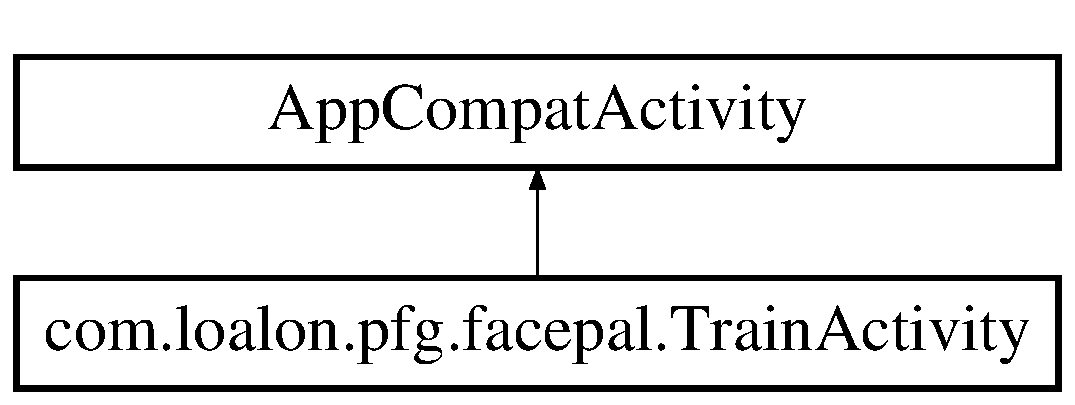
\includegraphics[height=2.000000cm]{classcom_1_1loalon_1_1pfg_1_1facepal_1_1_train_activity}
\end{center}
\end{figure}
\subsection*{Métodos protegidos}
\begin{DoxyCompactItemize}
\item 
void \mbox{\hyperlink{classcom_1_1loalon_1_1pfg_1_1facepal_1_1_train_activity_aed9fe1619d857821650314ca9b3537d7}{on\+Create}} (Bundle saved\+Instance\+State)
\end{DoxyCompactItemize}


\subsection{Descripción detallada}
Crea la actividad de entrenamiento de Face\+Pal. 

Created by Alonso on 02/04/2018. \begin{DoxyAuthor}{Autor}
Alonso Serrano 
\end{DoxyAuthor}
\begin{DoxyVersion}{Versión}
180418 
\end{DoxyVersion}


\subsection{Documentación de las funciones miembro}
\mbox{\Hypertarget{classcom_1_1loalon_1_1pfg_1_1facepal_1_1_train_activity_aed9fe1619d857821650314ca9b3537d7}\label{classcom_1_1loalon_1_1pfg_1_1facepal_1_1_train_activity_aed9fe1619d857821650314ca9b3537d7}} 
\index{com\+::loalon\+::pfg\+::facepal\+::\+Train\+Activity@{com\+::loalon\+::pfg\+::facepal\+::\+Train\+Activity}!on\+Create@{on\+Create}}
\index{on\+Create@{on\+Create}!com\+::loalon\+::pfg\+::facepal\+::\+Train\+Activity@{com\+::loalon\+::pfg\+::facepal\+::\+Train\+Activity}}
\subsubsection{\texorpdfstring{on\+Create()}{onCreate()}}
{\footnotesize\ttfamily void com.\+loalon.\+pfg.\+facepal.\+Train\+Activity.\+on\+Create (\begin{DoxyParamCaption}\item[{Bundle}]{saved\+Instance\+State }\end{DoxyParamCaption})\hspace{0.3cm}{\ttfamily [protected]}}


\hypertarget{classcom_1_1loalon_1_1pfg_1_1facepal_1_1_util}{}\section{Referencia de la Clase com.\+loalon.\+pfg.\+facepal.\+Util}
\label{classcom_1_1loalon_1_1pfg_1_1facepal_1_1_util}\index{com.\+loalon.\+pfg.\+facepal.\+Util@{com.\+loalon.\+pfg.\+facepal.\+Util}}


Clase que contiene metodos estaticos independientes del G\+UI Sirve como la clase \char`\"{}engine\char`\"{} para poder portarla a otras aplicaciones.  


\subsection*{Métodos públicos estáticos}
\begin{DoxyCompactItemize}
\item 
static byte \mbox{[}$\,$\mbox{]} \mbox{\hyperlink{classcom_1_1loalon_1_1pfg_1_1facepal_1_1_util_a363e942720417034c6c52fe4dd21df31}{to\+Base64}} (Bitmap bitmap)
\begin{DoxyCompactList}\small\item\em Convierte un bitmap a byte array base64 Requisito de Azure. \end{DoxyCompactList}\item 
static String \mbox{\hyperlink{classcom_1_1loalon_1_1pfg_1_1facepal_1_1_util_aa2f3ea68628c684b86868bf5d3a1cd5f}{get\+Base\+U\+RL}} ()
\begin{DoxyCompactList}\small\item\em Devuelve U\+RL base. \end{DoxyCompactList}\item 
static String \mbox{\hyperlink{classcom_1_1loalon_1_1pfg_1_1facepal_1_1_util_a537cee01d79a860eb281c942e97636eb}{get\+Key}} ()
\begin{DoxyCompactList}\small\item\em Devuelve clave de suscripcion. \end{DoxyCompactList}\item 
static String \mbox{\hyperlink{classcom_1_1loalon_1_1pfg_1_1facepal_1_1_util_a78dd2a2f40d6f82d71b7674ce40b46aa}{get\+Group\+Name}} ()
\begin{DoxyCompactList}\small\item\em Devuelve nombre de grupo de personas. \end{DoxyCompactList}\item 
static Bitmap \mbox{\hyperlink{classcom_1_1loalon_1_1pfg_1_1facepal_1_1_util_a57c1890189bffa4c69c51e286a2f6dbf}{detect\+Face}} (Bitmap bitmap)
\begin{DoxyCompactList}\small\item\em Deteccion de caras. \end{DoxyCompactList}\item 
static String \mbox{\hyperlink{classcom_1_1loalon_1_1pfg_1_1facepal_1_1_util_ac1062b1f3ee41b64274d734556cac898}{get\+Name}} (String person\+ID)
\begin{DoxyCompactList}\small\item\em Recupera el nombre real de una persona mediante su ID. \end{DoxyCompactList}\item 
static String \mbox{\hyperlink{classcom_1_1loalon_1_1pfg_1_1facepal_1_1_util_acedba139e29bc531032abf79980128d2}{identi\+Face}} (Bitmap bitmap)
\begin{DoxyCompactList}\small\item\em Identifica una persona mediante una cara recortada. \end{DoxyCompactList}\item 
static String \mbox{\hyperlink{classcom_1_1loalon_1_1pfg_1_1facepal_1_1_util_a59c6bb634708c5835281c91ead1b80bf}{train\+Group}} (String group\+Name)
\begin{DoxyCompactList}\small\item\em Indica a Azure que debe entrenar el grupo. \end{DoxyCompactList}\item 
static String \mbox{\hyperlink{classcom_1_1loalon_1_1pfg_1_1facepal_1_1_util_a94d73c1994c5e91f40cdf579e0aa7418}{add\+Face}} (String group\+Name, String person\+Name, Bitmap bitmap)
\begin{DoxyCompactList}\small\item\em Indica a Azure que debe entrenar el grupo. \end{DoxyCompactList}\item 
static String \mbox{\hyperlink{classcom_1_1loalon_1_1pfg_1_1facepal_1_1_util_ab74c33dc6a4bab04e396bce32b5dd62e}{get\+Person\+ID}} (String group\+Name, String name)
\begin{DoxyCompactList}\small\item\em Recupera el ID de una persona. \end{DoxyCompactList}\item 
static String \mbox{\hyperlink{classcom_1_1loalon_1_1pfg_1_1facepal_1_1_util_ac5f20400dac2f1de327eebbc22a26550}{add\+Person}} (String group\+Name, String name)
\begin{DoxyCompactList}\small\item\em Añade una persona al sistema. \end{DoxyCompactList}\item 
static String \mbox{\hyperlink{classcom_1_1loalon_1_1pfg_1_1facepal_1_1_util_aa4018f950fbd192cfd731e7ec401ea9e}{catch\+J\+S\+O\+Nerror}} (String json\+String)
\begin{DoxyCompactList}\small\item\em Verifica el contenido del J\+S\+ON recibido desde Azure, si contiene error lo interpreta y devuelve un mensaje claro sobre el error. \end{DoxyCompactList}\end{DoxyCompactItemize}


\subsection{Descripción detallada}
Clase que contiene metodos estaticos independientes del G\+UI Sirve como la clase \char`\"{}engine\char`\"{} para poder portarla a otras aplicaciones. 

Created by Alonso on 29/03/2018. \begin{DoxyAuthor}{Autor}
Alonso Serrano 
\end{DoxyAuthor}
\begin{DoxyVersion}{Versión}
180413 
\end{DoxyVersion}


\subsection{Documentación de las funciones miembro}
\mbox{\Hypertarget{classcom_1_1loalon_1_1pfg_1_1facepal_1_1_util_a94d73c1994c5e91f40cdf579e0aa7418}\label{classcom_1_1loalon_1_1pfg_1_1facepal_1_1_util_a94d73c1994c5e91f40cdf579e0aa7418}} 
\index{com\+::loalon\+::pfg\+::facepal\+::\+Util@{com\+::loalon\+::pfg\+::facepal\+::\+Util}!add\+Face@{add\+Face}}
\index{add\+Face@{add\+Face}!com\+::loalon\+::pfg\+::facepal\+::\+Util@{com\+::loalon\+::pfg\+::facepal\+::\+Util}}
\subsubsection{\texorpdfstring{add\+Face()}{addFace()}}
{\footnotesize\ttfamily static String com.\+loalon.\+pfg.\+facepal.\+Util.\+add\+Face (\begin{DoxyParamCaption}\item[{String}]{group\+Name,  }\item[{String}]{person\+Name,  }\item[{Bitmap}]{bitmap }\end{DoxyParamCaption})\hspace{0.3cm}{\ttfamily [static]}}



Indica a Azure que debe entrenar el grupo. 


\begin{DoxyParams}{Parámetros}
{\em group\+Name} & nombre del grupo de personas a entrenar \\
\hline
{\em bitmap} & imagen para añadir \\
\hline
{\em person\+Name} & nombre de la persona a añadir \\
\hline
\end{DoxyParams}
\begin{DoxyReturn}{Devuelve}
resultado de la operacion 
\end{DoxyReturn}
\mbox{\Hypertarget{classcom_1_1loalon_1_1pfg_1_1facepal_1_1_util_ac5f20400dac2f1de327eebbc22a26550}\label{classcom_1_1loalon_1_1pfg_1_1facepal_1_1_util_ac5f20400dac2f1de327eebbc22a26550}} 
\index{com\+::loalon\+::pfg\+::facepal\+::\+Util@{com\+::loalon\+::pfg\+::facepal\+::\+Util}!add\+Person@{add\+Person}}
\index{add\+Person@{add\+Person}!com\+::loalon\+::pfg\+::facepal\+::\+Util@{com\+::loalon\+::pfg\+::facepal\+::\+Util}}
\subsubsection{\texorpdfstring{add\+Person()}{addPerson()}}
{\footnotesize\ttfamily static String com.\+loalon.\+pfg.\+facepal.\+Util.\+add\+Person (\begin{DoxyParamCaption}\item[{String}]{group\+Name,  }\item[{String}]{name }\end{DoxyParamCaption})\hspace{0.3cm}{\ttfamily [static]}}



Añade una persona al sistema. 


\begin{DoxyParams}{Parámetros}
{\em group\+Name} & nombre del grupo de personas a entrenar \\
\hline
{\em name} & nombre de la persona a añadir \\
\hline
\end{DoxyParams}
\begin{DoxyReturn}{Devuelve}
resultado de la operacion, null si ha tenido exito 
\end{DoxyReturn}
\mbox{\Hypertarget{classcom_1_1loalon_1_1pfg_1_1facepal_1_1_util_aa4018f950fbd192cfd731e7ec401ea9e}\label{classcom_1_1loalon_1_1pfg_1_1facepal_1_1_util_aa4018f950fbd192cfd731e7ec401ea9e}} 
\index{com\+::loalon\+::pfg\+::facepal\+::\+Util@{com\+::loalon\+::pfg\+::facepal\+::\+Util}!catch\+J\+S\+O\+Nerror@{catch\+J\+S\+O\+Nerror}}
\index{catch\+J\+S\+O\+Nerror@{catch\+J\+S\+O\+Nerror}!com\+::loalon\+::pfg\+::facepal\+::\+Util@{com\+::loalon\+::pfg\+::facepal\+::\+Util}}
\subsubsection{\texorpdfstring{catch\+J\+S\+O\+Nerror()}{catchJSONerror()}}
{\footnotesize\ttfamily static String com.\+loalon.\+pfg.\+facepal.\+Util.\+catch\+J\+S\+O\+Nerror (\begin{DoxyParamCaption}\item[{String}]{json\+String }\end{DoxyParamCaption})\hspace{0.3cm}{\ttfamily [static]}}



Verifica el contenido del J\+S\+ON recibido desde Azure, si contiene error lo interpreta y devuelve un mensaje claro sobre el error. 


\begin{DoxyParams}{Parámetros}
{\em json\+String} & J\+S\+ON recibido \\
\hline
\end{DoxyParams}
\begin{DoxyReturn}{Devuelve}
mensaje de error o si no hay error el contenido del archivo J\+S\+ON 
\end{DoxyReturn}
\mbox{\Hypertarget{classcom_1_1loalon_1_1pfg_1_1facepal_1_1_util_a57c1890189bffa4c69c51e286a2f6dbf}\label{classcom_1_1loalon_1_1pfg_1_1facepal_1_1_util_a57c1890189bffa4c69c51e286a2f6dbf}} 
\index{com\+::loalon\+::pfg\+::facepal\+::\+Util@{com\+::loalon\+::pfg\+::facepal\+::\+Util}!detect\+Face@{detect\+Face}}
\index{detect\+Face@{detect\+Face}!com\+::loalon\+::pfg\+::facepal\+::\+Util@{com\+::loalon\+::pfg\+::facepal\+::\+Util}}
\subsubsection{\texorpdfstring{detect\+Face()}{detectFace()}}
{\footnotesize\ttfamily static Bitmap com.\+loalon.\+pfg.\+facepal.\+Util.\+detect\+Face (\begin{DoxyParamCaption}\item[{Bitmap}]{bitmap }\end{DoxyParamCaption})\hspace{0.3cm}{\ttfamily [static]}}



Deteccion de caras. 


\begin{DoxyParams}{Parámetros}
{\em bitmap} & imagen para detectar si existe una cara \\
\hline
\end{DoxyParams}
\begin{DoxyReturn}{Devuelve}
imagen recortada solo con un rostro o null si existen 0 o mas de 1 cara 
\end{DoxyReturn}
\mbox{\Hypertarget{classcom_1_1loalon_1_1pfg_1_1facepal_1_1_util_aa2f3ea68628c684b86868bf5d3a1cd5f}\label{classcom_1_1loalon_1_1pfg_1_1facepal_1_1_util_aa2f3ea68628c684b86868bf5d3a1cd5f}} 
\index{com\+::loalon\+::pfg\+::facepal\+::\+Util@{com\+::loalon\+::pfg\+::facepal\+::\+Util}!get\+Base\+U\+RL@{get\+Base\+U\+RL}}
\index{get\+Base\+U\+RL@{get\+Base\+U\+RL}!com\+::loalon\+::pfg\+::facepal\+::\+Util@{com\+::loalon\+::pfg\+::facepal\+::\+Util}}
\subsubsection{\texorpdfstring{get\+Base\+U\+R\+L()}{getBaseURL()}}
{\footnotesize\ttfamily static String com.\+loalon.\+pfg.\+facepal.\+Util.\+get\+Base\+U\+RL (\begin{DoxyParamCaption}{ }\end{DoxyParamCaption})\hspace{0.3cm}{\ttfamily [static]}}



Devuelve U\+RL base. 

\begin{DoxyReturn}{Devuelve}
U\+RL base 
\end{DoxyReturn}
\mbox{\Hypertarget{classcom_1_1loalon_1_1pfg_1_1facepal_1_1_util_a78dd2a2f40d6f82d71b7674ce40b46aa}\label{classcom_1_1loalon_1_1pfg_1_1facepal_1_1_util_a78dd2a2f40d6f82d71b7674ce40b46aa}} 
\index{com\+::loalon\+::pfg\+::facepal\+::\+Util@{com\+::loalon\+::pfg\+::facepal\+::\+Util}!get\+Group\+Name@{get\+Group\+Name}}
\index{get\+Group\+Name@{get\+Group\+Name}!com\+::loalon\+::pfg\+::facepal\+::\+Util@{com\+::loalon\+::pfg\+::facepal\+::\+Util}}
\subsubsection{\texorpdfstring{get\+Group\+Name()}{getGroupName()}}
{\footnotesize\ttfamily static String com.\+loalon.\+pfg.\+facepal.\+Util.\+get\+Group\+Name (\begin{DoxyParamCaption}{ }\end{DoxyParamCaption})\hspace{0.3cm}{\ttfamily [static]}}



Devuelve nombre de grupo de personas. 

\begin{DoxyReturn}{Devuelve}
nombre de grupo de personas 
\end{DoxyReturn}
\mbox{\Hypertarget{classcom_1_1loalon_1_1pfg_1_1facepal_1_1_util_a537cee01d79a860eb281c942e97636eb}\label{classcom_1_1loalon_1_1pfg_1_1facepal_1_1_util_a537cee01d79a860eb281c942e97636eb}} 
\index{com\+::loalon\+::pfg\+::facepal\+::\+Util@{com\+::loalon\+::pfg\+::facepal\+::\+Util}!get\+Key@{get\+Key}}
\index{get\+Key@{get\+Key}!com\+::loalon\+::pfg\+::facepal\+::\+Util@{com\+::loalon\+::pfg\+::facepal\+::\+Util}}
\subsubsection{\texorpdfstring{get\+Key()}{getKey()}}
{\footnotesize\ttfamily static String com.\+loalon.\+pfg.\+facepal.\+Util.\+get\+Key (\begin{DoxyParamCaption}{ }\end{DoxyParamCaption})\hspace{0.3cm}{\ttfamily [static]}}



Devuelve clave de suscripcion. 

\begin{DoxyReturn}{Devuelve}
clave de suscripcion 
\end{DoxyReturn}
\mbox{\Hypertarget{classcom_1_1loalon_1_1pfg_1_1facepal_1_1_util_ac1062b1f3ee41b64274d734556cac898}\label{classcom_1_1loalon_1_1pfg_1_1facepal_1_1_util_ac1062b1f3ee41b64274d734556cac898}} 
\index{com\+::loalon\+::pfg\+::facepal\+::\+Util@{com\+::loalon\+::pfg\+::facepal\+::\+Util}!get\+Name@{get\+Name}}
\index{get\+Name@{get\+Name}!com\+::loalon\+::pfg\+::facepal\+::\+Util@{com\+::loalon\+::pfg\+::facepal\+::\+Util}}
\subsubsection{\texorpdfstring{get\+Name()}{getName()}}
{\footnotesize\ttfamily static String com.\+loalon.\+pfg.\+facepal.\+Util.\+get\+Name (\begin{DoxyParamCaption}\item[{String}]{person\+ID }\end{DoxyParamCaption})\hspace{0.3cm}{\ttfamily [static]}}



Recupera el nombre real de una persona mediante su ID. 


\begin{DoxyParams}{Parámetros}
{\em person\+ID} & id de la persona \\
\hline
\end{DoxyParams}
\begin{DoxyReturn}{Devuelve}
nombre de la persona 
\end{DoxyReturn}
\mbox{\Hypertarget{classcom_1_1loalon_1_1pfg_1_1facepal_1_1_util_ab74c33dc6a4bab04e396bce32b5dd62e}\label{classcom_1_1loalon_1_1pfg_1_1facepal_1_1_util_ab74c33dc6a4bab04e396bce32b5dd62e}} 
\index{com\+::loalon\+::pfg\+::facepal\+::\+Util@{com\+::loalon\+::pfg\+::facepal\+::\+Util}!get\+Person\+ID@{get\+Person\+ID}}
\index{get\+Person\+ID@{get\+Person\+ID}!com\+::loalon\+::pfg\+::facepal\+::\+Util@{com\+::loalon\+::pfg\+::facepal\+::\+Util}}
\subsubsection{\texorpdfstring{get\+Person\+I\+D()}{getPersonID()}}
{\footnotesize\ttfamily static String com.\+loalon.\+pfg.\+facepal.\+Util.\+get\+Person\+ID (\begin{DoxyParamCaption}\item[{String}]{group\+Name,  }\item[{String}]{name }\end{DoxyParamCaption})\hspace{0.3cm}{\ttfamily [static]}}



Recupera el ID de una persona. 


\begin{DoxyParams}{Parámetros}
{\em group\+Name} & nombre del grupo de personas \\
\hline
{\em name} & nombre de la persona \\
\hline
\end{DoxyParams}
\begin{DoxyReturn}{Devuelve}
Id de la persona 
\end{DoxyReturn}
\mbox{\Hypertarget{classcom_1_1loalon_1_1pfg_1_1facepal_1_1_util_acedba139e29bc531032abf79980128d2}\label{classcom_1_1loalon_1_1pfg_1_1facepal_1_1_util_acedba139e29bc531032abf79980128d2}} 
\index{com\+::loalon\+::pfg\+::facepal\+::\+Util@{com\+::loalon\+::pfg\+::facepal\+::\+Util}!identi\+Face@{identi\+Face}}
\index{identi\+Face@{identi\+Face}!com\+::loalon\+::pfg\+::facepal\+::\+Util@{com\+::loalon\+::pfg\+::facepal\+::\+Util}}
\subsubsection{\texorpdfstring{identi\+Face()}{identiFace()}}
{\footnotesize\ttfamily static String com.\+loalon.\+pfg.\+facepal.\+Util.\+identi\+Face (\begin{DoxyParamCaption}\item[{Bitmap}]{bitmap }\end{DoxyParamCaption})\hspace{0.3cm}{\ttfamily [static]}}



Identifica una persona mediante una cara recortada. 


\begin{DoxyParams}{Parámetros}
{\em bitmap} & imagen de cara recortada \\
\hline
\end{DoxyParams}
\begin{DoxyReturn}{Devuelve}
identificador del mejor candidato 
\end{DoxyReturn}
\mbox{\Hypertarget{classcom_1_1loalon_1_1pfg_1_1facepal_1_1_util_a363e942720417034c6c52fe4dd21df31}\label{classcom_1_1loalon_1_1pfg_1_1facepal_1_1_util_a363e942720417034c6c52fe4dd21df31}} 
\index{com\+::loalon\+::pfg\+::facepal\+::\+Util@{com\+::loalon\+::pfg\+::facepal\+::\+Util}!to\+Base64@{to\+Base64}}
\index{to\+Base64@{to\+Base64}!com\+::loalon\+::pfg\+::facepal\+::\+Util@{com\+::loalon\+::pfg\+::facepal\+::\+Util}}
\subsubsection{\texorpdfstring{to\+Base64()}{toBase64()}}
{\footnotesize\ttfamily static byte \mbox{[}$\,$\mbox{]} com.\+loalon.\+pfg.\+facepal.\+Util.\+to\+Base64 (\begin{DoxyParamCaption}\item[{Bitmap}]{bitmap }\end{DoxyParamCaption})\hspace{0.3cm}{\ttfamily [static]}}



Convierte un bitmap a byte array base64 Requisito de Azure. 


\begin{DoxyParams}{Parámetros}
{\em bitmap} & imagen a enviar \\
\hline
\end{DoxyParams}
\begin{DoxyReturn}{Devuelve}
array de bytes en base64 
\end{DoxyReturn}
\mbox{\Hypertarget{classcom_1_1loalon_1_1pfg_1_1facepal_1_1_util_a59c6bb634708c5835281c91ead1b80bf}\label{classcom_1_1loalon_1_1pfg_1_1facepal_1_1_util_a59c6bb634708c5835281c91ead1b80bf}} 
\index{com\+::loalon\+::pfg\+::facepal\+::\+Util@{com\+::loalon\+::pfg\+::facepal\+::\+Util}!train\+Group@{train\+Group}}
\index{train\+Group@{train\+Group}!com\+::loalon\+::pfg\+::facepal\+::\+Util@{com\+::loalon\+::pfg\+::facepal\+::\+Util}}
\subsubsection{\texorpdfstring{train\+Group()}{trainGroup()}}
{\footnotesize\ttfamily static String com.\+loalon.\+pfg.\+facepal.\+Util.\+train\+Group (\begin{DoxyParamCaption}\item[{String}]{group\+Name }\end{DoxyParamCaption})\hspace{0.3cm}{\ttfamily [static]}}



Indica a Azure que debe entrenar el grupo. 


\begin{DoxyParams}{Parámetros}
{\em group\+Name} & nombre del grupo de personas a entrenar \\
\hline
\end{DoxyParams}
\begin{DoxyReturn}{Devuelve}
resultado de la operacion, null si ha tenido exito 
\end{DoxyReturn}

\chapter{Documentación de archivos}
\hypertarget{_face_b_t_8py}{}\section{Referencia del Archivo Face\+B\+T/\+Face\+BT.py}
\label{_face_b_t_8py}\index{Face\+B\+T/\+Face\+B\+T.\+py@{Face\+B\+T/\+Face\+B\+T.\+py}}
\subsection*{Clases}
\begin{DoxyCompactItemize}
\item 
class \mbox{\hyperlink{class_face_b_t_1_1_face_b_t}{Face\+B\+T.\+Face\+BT}}
\begin{DoxyCompactList}\small\item\em Clase principal de \mbox{\hyperlink{class_face_b_t_1_1_face_b_t}{Face\+BT}}. \end{DoxyCompactList}\end{DoxyCompactItemize}
\subsection*{Namespaces}
\begin{DoxyCompactItemize}
\item 
 \mbox{\hyperlink{namespace_face_b_t}{Face\+BT}}
\end{DoxyCompactItemize}
\subsection*{Funciones}
\begin{DoxyCompactItemize}
\item 
def \mbox{\hyperlink{namespace_face_b_t_ae0478ade43b4da93ebb363e389220087}{Face\+B\+T.\+main}} ()
\begin{DoxyCompactList}\small\item\em Funcion principal. \end{DoxyCompactList}\end{DoxyCompactItemize}
\subsection*{Variables}
\begin{DoxyCompactItemize}
\item 
\mbox{\hyperlink{namespace_face_b_t_a96f57377873e3c5cae0ad546f0a65bb7}{Face\+B\+T.\+camera}} = Pi\+Camera()
\end{DoxyCompactItemize}

\hypertarget{_about_activity_8java}{}\section{Referencia del Archivo face\+Pal/app/src/main/java/com/loalon/pfg/facepal/\+About\+Activity.java}
\label{_about_activity_8java}\index{face\+Pal/app/src/main/java/com/loalon/pfg/facepal/\+About\+Activity.\+java@{face\+Pal/app/src/main/java/com/loalon/pfg/facepal/\+About\+Activity.\+java}}
\subsection*{Clases}
\begin{DoxyCompactItemize}
\item 
class \mbox{\hyperlink{classcom_1_1loalon_1_1pfg_1_1facepal_1_1_about_activity}{com.\+loalon.\+pfg.\+facepal.\+About\+Activity}}
\begin{DoxyCompactList}\small\item\em Crea la actividad correspondiente para la pantalla acerca de... \end{DoxyCompactList}\end{DoxyCompactItemize}
\subsection*{Paquetes}
\begin{DoxyCompactItemize}
\item 
package \mbox{\hyperlink{namespacecom_1_1loalon_1_1pfg_1_1facepal}{com.\+loalon.\+pfg.\+facepal}}
\end{DoxyCompactItemize}

\hypertarget{_app_compat_preference_activity_8java}{}\section{Referencia del Archivo face\+Pal/app/src/main/java/com/loalon/pfg/facepal/\+App\+Compat\+Preference\+Activity.java}
\label{_app_compat_preference_activity_8java}\index{face\+Pal/app/src/main/java/com/loalon/pfg/facepal/\+App\+Compat\+Preference\+Activity.\+java@{face\+Pal/app/src/main/java/com/loalon/pfg/facepal/\+App\+Compat\+Preference\+Activity.\+java}}
\subsection*{Clases}
\begin{DoxyCompactItemize}
\item 
class \mbox{\hyperlink{classcom_1_1loalon_1_1pfg_1_1facepal_1_1_app_compat_preference_activity}{com.\+loalon.\+pfg.\+facepal.\+App\+Compat\+Preference\+Activity}}
\begin{DoxyCompactList}\small\item\em Creada por Android Studio para implementar el menu de configuración. \end{DoxyCompactList}\end{DoxyCompactItemize}
\subsection*{Paquetes}
\begin{DoxyCompactItemize}
\item 
package \mbox{\hyperlink{namespacecom_1_1loalon_1_1pfg_1_1facepal}{com.\+loalon.\+pfg.\+facepal}}
\end{DoxyCompactItemize}

\hypertarget{_async_add_face_8java}{}\section{Referencia del Archivo E\+:/\+One\+Drive.personal/\+One\+Drive/0.P\+F\+G/src/face\+Pal/app/src/main/java/com/loalon/pfg/facepal/\+Async\+Add\+Face.java}
\label{_async_add_face_8java}\index{E\+:/\+One\+Drive.\+personal/\+One\+Drive/0.\+P\+F\+G/src/face\+Pal/app/src/main/java/com/loalon/pfg/facepal/\+Async\+Add\+Face.\+java@{E\+:/\+One\+Drive.\+personal/\+One\+Drive/0.\+P\+F\+G/src/face\+Pal/app/src/main/java/com/loalon/pfg/facepal/\+Async\+Add\+Face.\+java}}
\subsection*{Clases}
\begin{DoxyCompactItemize}
\item 
class \mbox{\hyperlink{classcom_1_1loalon_1_1pfg_1_1facepal_1_1_async_add_face}{com.\+loalon.\+pfg.\+facepal.\+Async\+Add\+Face}}
\begin{DoxyCompactList}\small\item\em Tarea asincrona de añadir cara. \end{DoxyCompactList}\end{DoxyCompactItemize}
\subsection*{Paquetes}
\begin{DoxyCompactItemize}
\item 
package \mbox{\hyperlink{namespacecom_1_1loalon_1_1pfg_1_1facepal}{com.\+loalon.\+pfg.\+facepal}}
\end{DoxyCompactItemize}

\hypertarget{_async_add_person_8java}{}\section{Referencia del Archivo E\+:/\+One\+Drive.personal/\+One\+Drive/0.P\+F\+G/src/face\+Pal/app/src/main/java/com/loalon/pfg/facepal/\+Async\+Add\+Person.java}
\label{_async_add_person_8java}\index{E\+:/\+One\+Drive.\+personal/\+One\+Drive/0.\+P\+F\+G/src/face\+Pal/app/src/main/java/com/loalon/pfg/facepal/\+Async\+Add\+Person.\+java@{E\+:/\+One\+Drive.\+personal/\+One\+Drive/0.\+P\+F\+G/src/face\+Pal/app/src/main/java/com/loalon/pfg/facepal/\+Async\+Add\+Person.\+java}}
\subsection*{Clases}
\begin{DoxyCompactItemize}
\item 
class \mbox{\hyperlink{classcom_1_1loalon_1_1pfg_1_1facepal_1_1_async_add_person}{com.\+loalon.\+pfg.\+facepal.\+Async\+Add\+Person}}
\begin{DoxyCompactList}\small\item\em Tarea asincrona de añadir persona. \end{DoxyCompactList}\end{DoxyCompactItemize}
\subsection*{Paquetes}
\begin{DoxyCompactItemize}
\item 
package \mbox{\hyperlink{namespacecom_1_1loalon_1_1pfg_1_1facepal}{com.\+loalon.\+pfg.\+facepal}}
\end{DoxyCompactItemize}

\hypertarget{_async_face_croper_8java}{}\section{Referencia del Archivo face\+Pal/app/src/main/java/com/loalon/pfg/facepal/\+Async\+Face\+Croper.java}
\label{_async_face_croper_8java}\index{face\+Pal/app/src/main/java/com/loalon/pfg/facepal/\+Async\+Face\+Croper.\+java@{face\+Pal/app/src/main/java/com/loalon/pfg/facepal/\+Async\+Face\+Croper.\+java}}
\subsection*{Clases}
\begin{DoxyCompactItemize}
\item 
class \mbox{\hyperlink{classcom_1_1loalon_1_1pfg_1_1facepal_1_1_async_face_croper}{com.\+loalon.\+pfg.\+facepal.\+Async\+Face\+Croper}}
\begin{DoxyCompactList}\small\item\em Tarea asincrona de recortar cara. \end{DoxyCompactList}\item 
interface \mbox{\hyperlink{interfacecom_1_1loalon_1_1pfg_1_1facepal_1_1_async_face_croper_1_1_async_response}{com.\+loalon.\+pfg.\+facepal.\+Async\+Face\+Croper.\+Async\+Response}}
\end{DoxyCompactItemize}
\subsection*{Paquetes}
\begin{DoxyCompactItemize}
\item 
package \mbox{\hyperlink{namespacecom_1_1loalon_1_1pfg_1_1facepal}{com.\+loalon.\+pfg.\+facepal}}
\end{DoxyCompactItemize}

\hypertarget{_async_face_detector_8java}{}\section{Referencia del Archivo E\+:/\+One\+Drive.personal/\+One\+Drive/0.P\+F\+G/src/face\+Pal/app/src/main/java/com/loalon/pfg/facepal/\+Async\+Face\+Detector.java}
\label{_async_face_detector_8java}\index{E\+:/\+One\+Drive.\+personal/\+One\+Drive/0.\+P\+F\+G/src/face\+Pal/app/src/main/java/com/loalon/pfg/facepal/\+Async\+Face\+Detector.\+java@{E\+:/\+One\+Drive.\+personal/\+One\+Drive/0.\+P\+F\+G/src/face\+Pal/app/src/main/java/com/loalon/pfg/facepal/\+Async\+Face\+Detector.\+java}}
\subsection*{Clases}
\begin{DoxyCompactItemize}
\item 
class \mbox{\hyperlink{classcom_1_1loalon_1_1pfg_1_1facepal_1_1_async_face_detector}{com.\+loalon.\+pfg.\+facepal.\+Async\+Face\+Detector}}
\begin{DoxyCompactList}\small\item\em Tarea asincrona de D\+E\+T\+E\+C\+T\+AR cara. \end{DoxyCompactList}\end{DoxyCompactItemize}
\subsection*{Paquetes}
\begin{DoxyCompactItemize}
\item 
package \mbox{\hyperlink{namespacecom_1_1loalon_1_1pfg_1_1facepal}{com.\+loalon.\+pfg.\+facepal}}
\end{DoxyCompactItemize}

\hypertarget{_global_class_8java}{}\section{Referencia del Archivo face\+Pal/app/src/main/java/com/loalon/pfg/facepal/\+Global\+Class.java}
\label{_global_class_8java}\index{face\+Pal/app/src/main/java/com/loalon/pfg/facepal/\+Global\+Class.\+java@{face\+Pal/app/src/main/java/com/loalon/pfg/facepal/\+Global\+Class.\+java}}
\subsection*{Clases}
\begin{DoxyCompactItemize}
\item 
class \mbox{\hyperlink{classcom_1_1loalon_1_1pfg_1_1facepal_1_1_global_class}{com.\+loalon.\+pfg.\+facepal.\+Global\+Class}}
\begin{DoxyCompactList}\small\item\em Permite acceder de forma \char`\"{}global\char`\"{} al context de la aplicacion. \end{DoxyCompactList}\end{DoxyCompactItemize}
\subsection*{Paquetes}
\begin{DoxyCompactItemize}
\item 
package \mbox{\hyperlink{namespacecom_1_1loalon_1_1pfg_1_1facepal}{com.\+loalon.\+pfg.\+facepal}}
\end{DoxyCompactItemize}

\hypertarget{_main_activity_8java}{}\section{Referencia del Archivo E\+:/\+One\+Drive.personal/\+One\+Drive/0.P\+F\+G/src/face\+Pal/app/src/main/java/com/loalon/pfg/facepal/\+Main\+Activity.java}
\label{_main_activity_8java}\index{E\+:/\+One\+Drive.\+personal/\+One\+Drive/0.\+P\+F\+G/src/face\+Pal/app/src/main/java/com/loalon/pfg/facepal/\+Main\+Activity.\+java@{E\+:/\+One\+Drive.\+personal/\+One\+Drive/0.\+P\+F\+G/src/face\+Pal/app/src/main/java/com/loalon/pfg/facepal/\+Main\+Activity.\+java}}
\subsection*{Clases}
\begin{DoxyCompactItemize}
\item 
class \mbox{\hyperlink{classcom_1_1loalon_1_1pfg_1_1facepal_1_1_main_activity}{com.\+loalon.\+pfg.\+facepal.\+Main\+Activity}}
\begin{DoxyCompactList}\small\item\em Crea la actividad principal de Face\+Pal. \end{DoxyCompactList}\end{DoxyCompactItemize}
\subsection*{Paquetes}
\begin{DoxyCompactItemize}
\item 
package \mbox{\hyperlink{namespacecom_1_1loalon_1_1pfg_1_1facepal}{com.\+loalon.\+pfg.\+facepal}}
\end{DoxyCompactItemize}

\hypertarget{_mini_snack_8java}{}\section{Referencia del Archivo E\+:/\+One\+Drive.personal/\+One\+Drive/0.P\+F\+G/src/face\+Pal/app/src/main/java/com/loalon/pfg/facepal/\+Mini\+Snack.java}
\label{_mini_snack_8java}\index{E\+:/\+One\+Drive.\+personal/\+One\+Drive/0.\+P\+F\+G/src/face\+Pal/app/src/main/java/com/loalon/pfg/facepal/\+Mini\+Snack.\+java@{E\+:/\+One\+Drive.\+personal/\+One\+Drive/0.\+P\+F\+G/src/face\+Pal/app/src/main/java/com/loalon/pfg/facepal/\+Mini\+Snack.\+java}}
\subsection*{Clases}
\begin{DoxyCompactItemize}
\item 
class \mbox{\hyperlink{classcom_1_1loalon_1_1pfg_1_1facepal_1_1_mini_snack}{com.\+loalon.\+pfg.\+facepal.\+Mini\+Snack}}
\begin{DoxyCompactList}\small\item\em Crea objetos Snackbar con un duración indeterminada hasta que el usuario pulsa el boton OK El proposito de los Minisnacks es informar y que el usuario no realice otras acciones hasta comprender el mensaje que se le devuelve. \end{DoxyCompactList}\end{DoxyCompactItemize}
\subsection*{Paquetes}
\begin{DoxyCompactItemize}
\item 
package \mbox{\hyperlink{namespacecom_1_1loalon_1_1pfg_1_1facepal}{com.\+loalon.\+pfg.\+facepal}}
\end{DoxyCompactItemize}

\hypertarget{_settings_activity_8java}{}\section{Referencia del Archivo E\+:/\+One\+Drive.personal/\+One\+Drive/0.P\+F\+G/src/face\+Pal/app/src/main/java/com/loalon/pfg/facepal/\+Settings\+Activity.java}
\label{_settings_activity_8java}\index{E\+:/\+One\+Drive.\+personal/\+One\+Drive/0.\+P\+F\+G/src/face\+Pal/app/src/main/java/com/loalon/pfg/facepal/\+Settings\+Activity.\+java@{E\+:/\+One\+Drive.\+personal/\+One\+Drive/0.\+P\+F\+G/src/face\+Pal/app/src/main/java/com/loalon/pfg/facepal/\+Settings\+Activity.\+java}}
\subsection*{Clases}
\begin{DoxyCompactItemize}
\item 
class \mbox{\hyperlink{classcom_1_1loalon_1_1pfg_1_1facepal_1_1_settings_activity}{com.\+loalon.\+pfg.\+facepal.\+Settings\+Activity}}
\begin{DoxyCompactList}\small\item\em Creada por Android Studio para implementar el menu de configuración Esta clse contiene mas codigo del necesario, pero se mantiene para añadir mas opciones de configuracion en el futuro. \end{DoxyCompactList}\item 
class {\bfseries com.\+loalon.\+pfg.\+facepal.\+Settings\+Activity.\+General\+Preference\+Fragment}
\begin{DoxyCompactList}\small\item\em This fragment shows general preferences only. \end{DoxyCompactList}\item 
class {\bfseries com.\+loalon.\+pfg.\+facepal.\+Settings\+Activity.\+Notification\+Preference\+Fragment}
\begin{DoxyCompactList}\small\item\em This fragment shows notification preferences only. \end{DoxyCompactList}\item 
class {\bfseries com.\+loalon.\+pfg.\+facepal.\+Settings\+Activity.\+Data\+Sync\+Preference\+Fragment}
\begin{DoxyCompactList}\small\item\em This fragment shows data and sync preferences only. \end{DoxyCompactList}\end{DoxyCompactItemize}
\subsection*{Paquetes}
\begin{DoxyCompactItemize}
\item 
package \mbox{\hyperlink{namespacecom_1_1loalon_1_1pfg_1_1facepal}{com.\+loalon.\+pfg.\+facepal}}
\end{DoxyCompactItemize}

\hypertarget{_train_activity_8java}{}\section{Referencia del Archivo E\+:/\+One\+Drive.personal/\+One\+Drive/0.P\+F\+G/src/face\+Pal/app/src/main/java/com/loalon/pfg/facepal/\+Train\+Activity.java}
\label{_train_activity_8java}\index{E\+:/\+One\+Drive.\+personal/\+One\+Drive/0.\+P\+F\+G/src/face\+Pal/app/src/main/java/com/loalon/pfg/facepal/\+Train\+Activity.\+java@{E\+:/\+One\+Drive.\+personal/\+One\+Drive/0.\+P\+F\+G/src/face\+Pal/app/src/main/java/com/loalon/pfg/facepal/\+Train\+Activity.\+java}}
\subsection*{Clases}
\begin{DoxyCompactItemize}
\item 
class \mbox{\hyperlink{classcom_1_1loalon_1_1pfg_1_1facepal_1_1_train_activity}{com.\+loalon.\+pfg.\+facepal.\+Train\+Activity}}
\begin{DoxyCompactList}\small\item\em Crea la actividad de entrenamiento de Face\+Pal. \end{DoxyCompactList}\end{DoxyCompactItemize}
\subsection*{Paquetes}
\begin{DoxyCompactItemize}
\item 
package \mbox{\hyperlink{namespacecom_1_1loalon_1_1pfg_1_1facepal}{com.\+loalon.\+pfg.\+facepal}}
\end{DoxyCompactItemize}

\hypertarget{_util_8java}{}\section{Referencia del Archivo E\+:/\+One\+Drive.personal/\+One\+Drive/0.P\+F\+G/src/face\+Pal/app/src/main/java/com/loalon/pfg/facepal/\+Util.java}
\label{_util_8java}\index{E\+:/\+One\+Drive.\+personal/\+One\+Drive/0.\+P\+F\+G/src/face\+Pal/app/src/main/java/com/loalon/pfg/facepal/\+Util.\+java@{E\+:/\+One\+Drive.\+personal/\+One\+Drive/0.\+P\+F\+G/src/face\+Pal/app/src/main/java/com/loalon/pfg/facepal/\+Util.\+java}}
\subsection*{Clases}
\begin{DoxyCompactItemize}
\item 
class \mbox{\hyperlink{classcom_1_1loalon_1_1pfg_1_1facepal_1_1_util}{com.\+loalon.\+pfg.\+facepal.\+Util}}
\begin{DoxyCompactList}\small\item\em Clase que contiene metodos estaticos independientes del G\+UI Sirve como la clase \char`\"{}engine\char`\"{} para poder portarla a otras aplicaciones. \end{DoxyCompactList}\end{DoxyCompactItemize}
\subsection*{Paquetes}
\begin{DoxyCompactItemize}
\item 
package \mbox{\hyperlink{namespacecom_1_1loalon_1_1pfg_1_1facepal}{com.\+loalon.\+pfg.\+facepal}}
\end{DoxyCompactItemize}

\hypertarget{facepi_8py}{}\section{Referencia del Archivo Face\+Pi/facepi.py}
\label{facepi_8py}\index{Face\+Pi/facepi.\+py@{Face\+Pi/facepi.\+py}}
\subsection*{Clases}
\begin{DoxyCompactItemize}
\item 
class \mbox{\hyperlink{classfacepi_1_1_face_pi}{facepi.\+Face\+Pi}}
\begin{DoxyCompactList}\small\item\em Clase principal de \mbox{\hyperlink{classfacepi_1_1_face_pi}{Face\+Pi}}. \end{DoxyCompactList}\end{DoxyCompactItemize}
\subsection*{Namespaces}
\begin{DoxyCompactItemize}
\item 
 \mbox{\hyperlink{namespacefacepi}{facepi}}
\end{DoxyCompactItemize}
\subsection*{Variables}
\begin{DoxyCompactItemize}
\item 
\mbox{\hyperlink{namespacefacepi_a15b6f38df49cdb5819542c3bb5f9de38}{facepi.\+app}} = Q\+Application(sys.\+argv)
\item 
\mbox{\hyperlink{namespacefacepi_ad59c23499aea037ab53a4bbf70c206ec}{facepi.\+ex}} = Face\+Pi()
\end{DoxyCompactItemize}

\hypertarget{_face_recon_8py}{}\section{Referencia del Archivo Face\+Recon/\+Face\+Recon.py}
\label{_face_recon_8py}\index{Face\+Recon/\+Face\+Recon.\+py@{Face\+Recon/\+Face\+Recon.\+py}}
\subsection*{Namespaces}
\begin{DoxyCompactItemize}
\item 
 \mbox{\hyperlink{namespace_face_recon}{Face\+Recon}}
\end{DoxyCompactItemize}
\subsection*{Variables}
\begin{DoxyCompactItemize}
\item 
\mbox{\hyperlink{namespace_face_recon_ac6ec5c173cf48f7c65fc970e1e079ca9}{Face\+Recon.\+camera}} = Pi\+Camera()
\begin{DoxyCompactList}\small\item\em C\+O\+N\+F\+I\+G\+U\+R\+A\+C\+I\+ON. \end{DoxyCompactList}\item 
\mbox{\hyperlink{namespace_face_recon_a6401bc73862ba52d12acc4e195359b84}{Face\+Recon.\+resolution}}
\item 
\mbox{\hyperlink{namespace_face_recon_aa83a22879c0d6299597d46b065e09c4c}{Face\+Recon.\+font}} = cv2.\+F\+O\+N\+T\+\_\+\+H\+E\+R\+S\+H\+E\+Y\+\_\+\+S\+I\+M\+P\+L\+EX
\item 
\mbox{\hyperlink{namespace_face_recon_a020b74724169b8fc02c88453680fa3cc}{Face\+Recon.\+config}} = configparser.\+Config\+Parser()
\item 
\mbox{\hyperlink{namespace_face_recon_a6a0cb127a374ad0eb5705d0f49a40040}{Face\+Recon.\+cfg}} = config\mbox{[}\textquotesingle{}C\+O\+N\+F\+IG\textquotesingle{}\mbox{]}
\item 
\mbox{\hyperlink{namespace_face_recon_aaadefd1ee1352d2f1b2fdf3ea4db8390}{Face\+Recon.\+fn}} = cfg\mbox{[}\textquotesingle{}facedetector\textquotesingle{}\mbox{]}
\item 
\mbox{\hyperlink{namespace_face_recon_a52d7b32070be8a278850cdb6afd2d301}{Face\+Recon.\+face\+Detector}} = os.\+path.\+join(os.\+path.\+dirname(\+\_\+\+\_\+file\+\_\+\+\_\+), fn)
\item 
\mbox{\hyperlink{namespace_face_recon_a5c8b2fa43564cbbd3abf3d1cacef7e8c}{Face\+Recon.\+s\+Key}} = cfg\mbox{[}\textquotesingle{}skey\textquotesingle{}\mbox{]}
\item 
\mbox{\hyperlink{namespace_face_recon_a78159752a247e46ae64caea5570a6889}{Face\+Recon.\+server}} = cfg\mbox{[}\textquotesingle{}server\textquotesingle{}\mbox{]}
\item 
\mbox{\hyperlink{namespace_face_recon_ae44f8e751a650fcfa6bc7d2a61242cc1}{Face\+Recon.\+group\+Name}} = cfg\mbox{[}\textquotesingle{}groupname\textquotesingle{}\mbox{]}
\item 
int \mbox{\hyperlink{namespace_face_recon_a1cec4fb530e8a7a1b10ac48890f36e7b}{Face\+Recon.\+wait\+Time}} = 20
\item 
\mbox{\hyperlink{namespace_face_recon_ac1dfb5855321e10d5338ad161bfa8151}{Face\+Recon.\+now}} = datetime.\+now()
\begin{DoxyCompactList}\small\item\em C\+O\+M\+P\+R\+O\+B\+A\+C\+I\+ON D\+I\+R\+E\+C\+T\+O\+R\+I\+OS. \end{DoxyCompactList}\item 
string \mbox{\hyperlink{namespace_face_recon_af54252e1ad4d24d516c64eaaa88905ce}{Face\+Recon.\+now\+Str}} = \textquotesingle{}\+\_\+\textquotesingle{}+str(now.\+year)+str(now.\+month)+str(now.\+day)+\textquotesingle{}\+\_\+\textquotesingle{}+str(now.\+hour)+str(now.\+minute)+str(now.\+second)
\item 
\mbox{\hyperlink{namespace_face_recon_a65dbfeade36a516a4fbd5cd1c44c5682}{Face\+Recon.\+img}} = fc.\+capture\+Image(camera)
\item 
\mbox{\hyperlink{namespace_face_recon_aaf2856e061dd5456e2ff875905fcc51b}{Face\+Recon.\+face\+List}} = fc.\+face\+Detect(face\+Detector, img, cv2)
\item 
bool \mbox{\hyperlink{namespace_face_recon_ac4b8075620307b113830af1893363bbe}{Face\+Recon.\+person\+Detected}} = False
\item 
\mbox{\hyperlink{namespace_face_recon_ad661554f5aa9213b00b4d791a65a29eb}{Face\+Recon.\+is\+Person}} = F\+C\+T.\+identify\+Face(CF, group\+Name, face)
\end{DoxyCompactItemize}

\hypertarget{face_8py}{}\section{Referencia del Archivo F\+C\+Module/\+F\+C\+Module/face.py}
\label{face_8py}\index{F\+C\+Module/\+F\+C\+Module/face.\+py@{F\+C\+Module/\+F\+C\+Module/face.\+py}}
\subsection*{Clases}
\begin{DoxyCompactItemize}
\item 
class \mbox{\hyperlink{class_f_c_module_1_1face_1_1_face}{F\+C\+Module.\+face.\+Face}}
\begin{DoxyCompactList}\small\item\em Clase \mbox{\hyperlink{class_f_c_module_1_1face_1_1_face}{Face}}. \end{DoxyCompactList}\end{DoxyCompactItemize}
\subsection*{Namespaces}
\begin{DoxyCompactItemize}
\item 
 \mbox{\hyperlink{namespace_f_c_module_1_1face}{F\+C\+Module.\+face}}
\end{DoxyCompactItemize}

\hypertarget{face_crop_8py}{}\section{Referencia del Archivo E\+:/\+One\+Drive.personal/\+One\+Drive/0.P\+F\+G/src/\+F\+C\+Module/\+F\+C\+Module/face\+Crop.py}
\label{face_crop_8py}\index{E\+:/\+One\+Drive.\+personal/\+One\+Drive/0.\+P\+F\+G/src/\+F\+C\+Module/\+F\+C\+Module/face\+Crop.\+py@{E\+:/\+One\+Drive.\+personal/\+One\+Drive/0.\+P\+F\+G/src/\+F\+C\+Module/\+F\+C\+Module/face\+Crop.\+py}}
\subsection*{Namespaces}
\begin{DoxyCompactItemize}
\item 
 \mbox{\hyperlink{namespace_f_c_module_1_1face_crop}{F\+C\+Module.\+face\+Crop}}
\item 
 \mbox{\hyperlink{namespaceface_crop}{face\+Crop}}
\begin{DoxyCompactList}\small\item\em Contiene las funciones de gestión de las imágenes relacionadas con el recorte de caras. \end{DoxyCompactList}\end{DoxyCompactItemize}
\subsection*{Funciones}
\begin{DoxyCompactItemize}
\item 
def \mbox{\hyperlink{namespace_f_c_module_1_1face_crop_a9bf6ee5d5b014b164481d2b04e342176}{F\+C\+Module.\+face\+Crop.\+capture\+Image}} (camera)
\begin{DoxyCompactList}\small\item\em Captura una imagen desde la camara de Raspberry Pi. \end{DoxyCompactList}\item 
def \mbox{\hyperlink{namespace_f_c_module_1_1face_crop_a8ea1491e88b53ba928c36fea4fab8f50}{F\+C\+Module.\+face\+Crop.\+face\+Detect}} (face\+Detector, image, cv2)
\begin{DoxyCompactList}\small\item\em Detecta caras, genera objetos Face con las coordenadas de cada cara y devuelve un lista con los objetos Face. \end{DoxyCompactList}\item 
def \mbox{\hyperlink{namespace_f_c_module_1_1face_crop_a228a8265b22b6f5b14306893fb8df335}{F\+C\+Module.\+face\+Crop.\+face\+Crop}} (image, cv2, face\+List)
\begin{DoxyCompactList}\small\item\em Genera archivos conlos recortes y modifica la lista de caras indicando los archivos asociados. \end{DoxyCompactList}\end{DoxyCompactItemize}

\hypertarget{_f_c_tools_8py}{}\section{Referencia del Archivo E\+:/\+One\+Drive.personal/\+One\+Drive/0.P\+F\+G/src/\+F\+C\+Module/\+F\+C\+Module/\+F\+C\+Tools.py}
\label{_f_c_tools_8py}\index{E\+:/\+One\+Drive.\+personal/\+One\+Drive/0.\+P\+F\+G/src/\+F\+C\+Module/\+F\+C\+Module/\+F\+C\+Tools.\+py@{E\+:/\+One\+Drive.\+personal/\+One\+Drive/0.\+P\+F\+G/src/\+F\+C\+Module/\+F\+C\+Module/\+F\+C\+Tools.\+py}}
\subsection*{Namespaces}
\begin{DoxyCompactItemize}
\item 
 \mbox{\hyperlink{namespace_f_c_module_1_1_f_c_tools}{F\+C\+Module.\+F\+C\+Tools}}
\item 
 \mbox{\hyperlink{namespace_f_c_tools}{F\+C\+Tools}}
\begin{DoxyCompactList}\small\item\em Contiene funciones para la puesta en marcha, el entrenamiento del sistema y funciones necesarias para el reconocimiento facial. \end{DoxyCompactList}\end{DoxyCompactItemize}
\subsection*{Funciones}
\begin{DoxyCompactItemize}
\item 
def \mbox{\hyperlink{namespace_f_c_module_1_1_f_c_tools_a97937928e5d262ee170874d1a84cf612}{F\+C\+Module.\+F\+C\+Tools.\+test\+Azure}} (service)
\begin{DoxyCompactList}\small\item\em Realiza un test de funcionamiento, imprime los resultados por pantalla. \end{DoxyCompactList}\item 
def \mbox{\hyperlink{namespace_f_c_module_1_1_f_c_tools_a67657f08b02e1202300530334a92de19}{F\+C\+Module.\+F\+C\+Tools.\+get\+Person\+ID}} (service, person\+Group, person\+Name)
\begin{DoxyCompactList}\small\item\em Realiza un test de funcionamiento, imprime los resultados por pantalla. \end{DoxyCompactList}\item 
def \mbox{\hyperlink{namespace_f_c_module_1_1_f_c_tools_af728b8917192873f11795aef2dd201ce}{F\+C\+Module.\+F\+C\+Tools.\+get\+Name\+By\+ID}} (service, person\+Group, person\+ID)
\begin{DoxyCompactList}\small\item\em Recupera el nombre a partir de un person\+ID. \end{DoxyCompactList}\item 
def \mbox{\hyperlink{namespace_f_c_module_1_1_f_c_tools_a2f1857b9750405992109bb659d4a2cfa}{F\+C\+Module.\+F\+C\+Tools.\+create\+Person\+Group}} (service, person\+Group)
\begin{DoxyCompactList}\small\item\em Crea un grupo de entrenamiento. \end{DoxyCompactList}\item 
def \mbox{\hyperlink{namespace_f_c_module_1_1_f_c_tools_a890f0f5e33c8b92c05c00876daeb756a}{F\+C\+Module.\+F\+C\+Tools.\+create\+Person}} (service, person\+Group, person\+Name)
\begin{DoxyCompactList}\small\item\em Crea a una persona. \end{DoxyCompactList}\item 
def \mbox{\hyperlink{namespace_f_c_module_1_1_f_c_tools_adeeadfac92a0113ba74f1b140c09b14f}{F\+C\+Module.\+F\+C\+Tools.\+add\+Face}} (service, person\+Group, person\+Name, image)
\begin{DoxyCompactList}\small\item\em Agrega a una persona. \end{DoxyCompactList}\item 
def \mbox{\hyperlink{namespace_f_c_module_1_1_f_c_tools_aedafa1474c8976ae1f9c1a859cc26984}{F\+C\+Module.\+F\+C\+Tools.\+delete\+Person}} (service, person\+Group, person\+Name)
\begin{DoxyCompactList}\small\item\em Borra a una persona. \end{DoxyCompactList}\item 
def \mbox{\hyperlink{namespace_f_c_module_1_1_f_c_tools_a780cf43ca7953c654750759dc80a0f48}{F\+C\+Module.\+F\+C\+Tools.\+delete\+Person\+Group}} (service, person\+Group)
\begin{DoxyCompactList}\small\item\em Borra a un grupo. \end{DoxyCompactList}\item 
def \mbox{\hyperlink{namespace_f_c_module_1_1_f_c_tools_ab3df8ddd7530893bcd38b5e5321f9576}{F\+C\+Module.\+F\+C\+Tools.\+identify\+Face}} (service, person\+Group, face)
\begin{DoxyCompactList}\small\item\em Esta función conecta con Azure, identifica la cara y pasa el nombre identificado al objeto Face correspondiente. \end{DoxyCompactList}\item 
def \mbox{\hyperlink{namespace_f_c_module_1_1_f_c_tools_a476cbac52df88ddaae5b43da6465013e}{F\+C\+Module.\+F\+C\+Tools.\+paint\+Image}} (cv, font, img, face)
\begin{DoxyCompactList}\small\item\em Esta función toma las coordenadas de un objeto Face y dibuja un rectángulo que enmarca la cara, además de escribir el nombre correspondiente a la cara. \end{DoxyCompactList}\item 
def \mbox{\hyperlink{namespace_f_c_module_1_1_f_c_tools_a10adfb32d85cc6173537e97ee7afea11}{F\+C\+Module.\+F\+C\+Tools.\+paint\+All\+Faces}} (cv, font, img, face\+List)
\begin{DoxyCompactList}\small\item\em Pinta un rectangulo sobre todas las caras y su nombre. \end{DoxyCompactList}\item 
def \mbox{\hyperlink{namespace_f_c_module_1_1_f_c_tools_a84b5fde279bce289df81e5c2f9ffe09d}{F\+C\+Module.\+F\+C\+Tools.\+list\+Persons}} (service, person\+Group)
\begin{DoxyCompactList}\small\item\em Devuelve un listado de personas de un grupo. \end{DoxyCompactList}\item 
def \mbox{\hyperlink{namespace_f_c_module_1_1_f_c_tools_a638f52cb88b6812ebd83e2967bd95b51}{F\+C\+Module.\+F\+C\+Tools.\+detect\+Person}} (service, person\+Group, file)
\begin{DoxyCompactList}\small\item\em Detecta a una persona en un archivo. \end{DoxyCompactList}\end{DoxyCompactItemize}

%--- End generated contents ---

% Index
\backmatter
\newpage
\phantomsection
\clearemptydoublepage
\addcontentsline{toc}{chapter}{Índice}
\printindex

\end{document}
